\documentclass[11pt,a4paper]{article}
\usepackage[margin=22mm]{geometry}
\usepackage{fontspec}
\setmainfont{Latin Modern Roman}
\setsansfont{Latin Modern Sans}
\setmonofont{Latin Modern Mono}
\usepackage{amsmath,amssymb}
\usepackage{unicode-math}
\setmathfont{Latin Modern Math}
\usepackage{longtable,array,fvextra,adjustbox,needspace}
\usepackage{pgfplots}
\usepackage{pdflscape}
\pgfplotsset{compat=1.18}
\usepackage[colorlinks=true,linkcolor=blue,urlcolor=blue,unicode=true]{hyperref}
\usepackage{xurl}
\newcounter{listing}
\newcounter{scripttable}
\definecolor{pcd1}{HTML}{005A78}
\definecolor{pcd2}{HTML}{6B2CB1}
\definecolor{pcd3}{HTML}{447766}
\definecolor{pcd4}{HTML}{9A3E20}
\definecolor{pcd5}{HTML}{756000}
\setlength{\parindent}{0pt}
\setlength{\parskip}{0.65em}
\setlength{\emergencystretch}{3em}
\begin{document}
\hypersetup{pdftitle={Linear Regression Foundations · TERMIN 1},pdfsubject={Authored thematic script},pdfcreator={Project Chemie Digital LaTeX exporter}}
\title{Linear Regression Foundations \ensuremath{\cdot} TERMIN 1}
\author{}
\date{}
\maketitle
\tableofcontents
\clearpage
\section{From a time trend to a criterion}
\textbf{Linear Regression}


Today we turn a time trend into a reproducible fitted model. We first agree what a good line means, then acquire enough matrix language to build a design matrix and derive the normal equations. The final applications change the known model terms without changing the linear coefficient problem. Uncertainty belongs to the next appointment.
\textbf{A signal drifts during a run}


During one run, we recorded the detector signal at the start and then once per minute. The figure pairs the detector setup with the five readings: 1.10, 2.80, 5.20, 6.90 and 9.00 mV at 0, 1, 2, 3 and 4 min, respectively. How can we predict the signal at 2.5 min, between two recorded times? A model describes signal as a function of time. We can evaluate it inside the measured interval (interpolation) or outside it (extrapolation). The dashed extension in the figure is an extrapolation beyond the last reading. Adding a model raises the next question: how do we choose a line that fits the measured points?


\hyperref[material-0cbd8025474be43ec999bee5b494a4a7786a19b561b67923fea96c6f1109b2da]{Fig.~\ref*{material-0cbd8025474be43ec999bee5b494a4a7786a19b561b67923fea96c6f1109b2da}}


\par\medskip
\Needspace{10cm}
\refstepcounter{figure}\label{material-0cbd8025474be43ec999bee5b494a4a7786a19b561b67923fea96c6f1109b2da}
\noindent\textbf{Fig.~\ref*{material-0cbd8025474be43ec999bee5b494a4a7786a19b561b67923fea96c6f1109b2da}.} Detector setup and signal readings during one run\par\nopagebreak
\begin{center}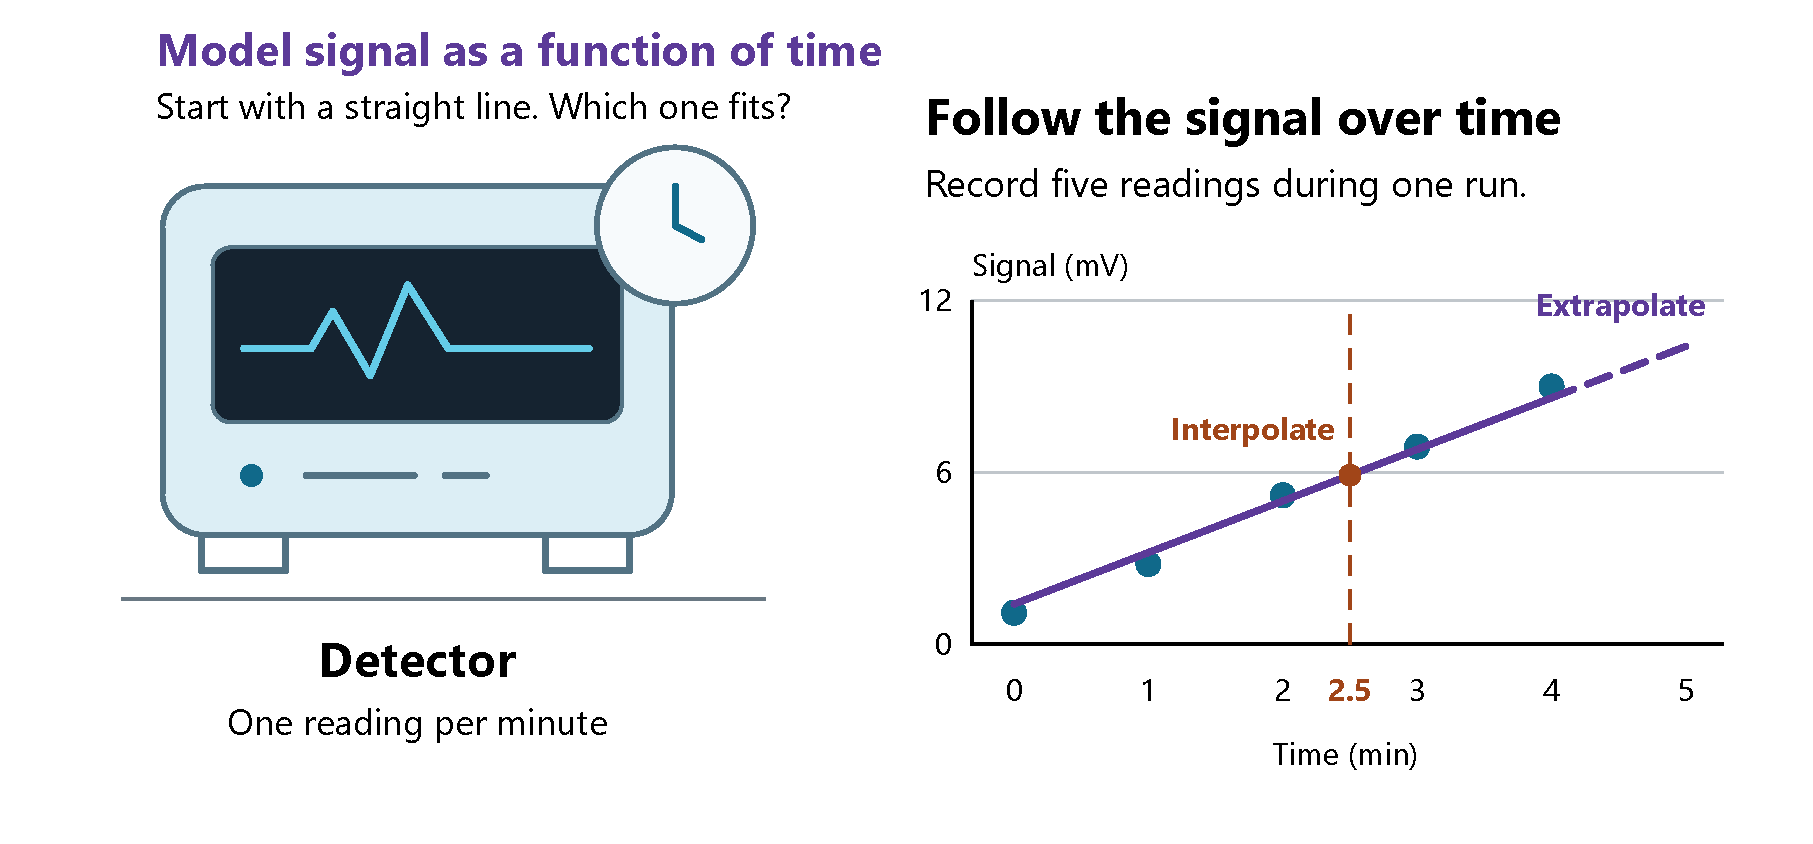
\includegraphics[width=\linewidth,height=.62\textheight,keepaspectratio]{asset-22eba6f57c5d2df1fc31c83d3bd1a52ab695d8cc1103a46db4517b31498bae76.pdf}\end{center}

\medskip

\textbf{Estimate a model from measurements}


To describe the measured trend with a straight line, we estimate two numbers using all five time–signal pairs. The intercept gives the modelled signal at zero minutes in mV. The slope gives the modelled change in signal per minute in mV/min. The schematic shows how the measurements inform both coefficients. In the interactive plot, you can change each one and see what happens to the line.


\hyperref[material-f5bdf71d5aa2d395d0ab9ff3f68f6df7d98edf31b12c0d65cbb324a513497396]{Fig.~\ref*{material-f5bdf71d5aa2d395d0ab9ff3f68f6df7d98edf31b12c0d65cbb324a513497396}}


\par\medskip
\Needspace{10cm}
\refstepcounter{figure}\label{material-f5bdf71d5aa2d395d0ab9ff3f68f6df7d98edf31b12c0d65cbb324a513497396}
\noindent\textbf{Fig.~\ref*{material-f5bdf71d5aa2d395d0ab9ff3f68f6df7d98edf31b12c0d65cbb324a513497396}.} How the measured pairs inform the line coefficients\par\nopagebreak
\begin{center}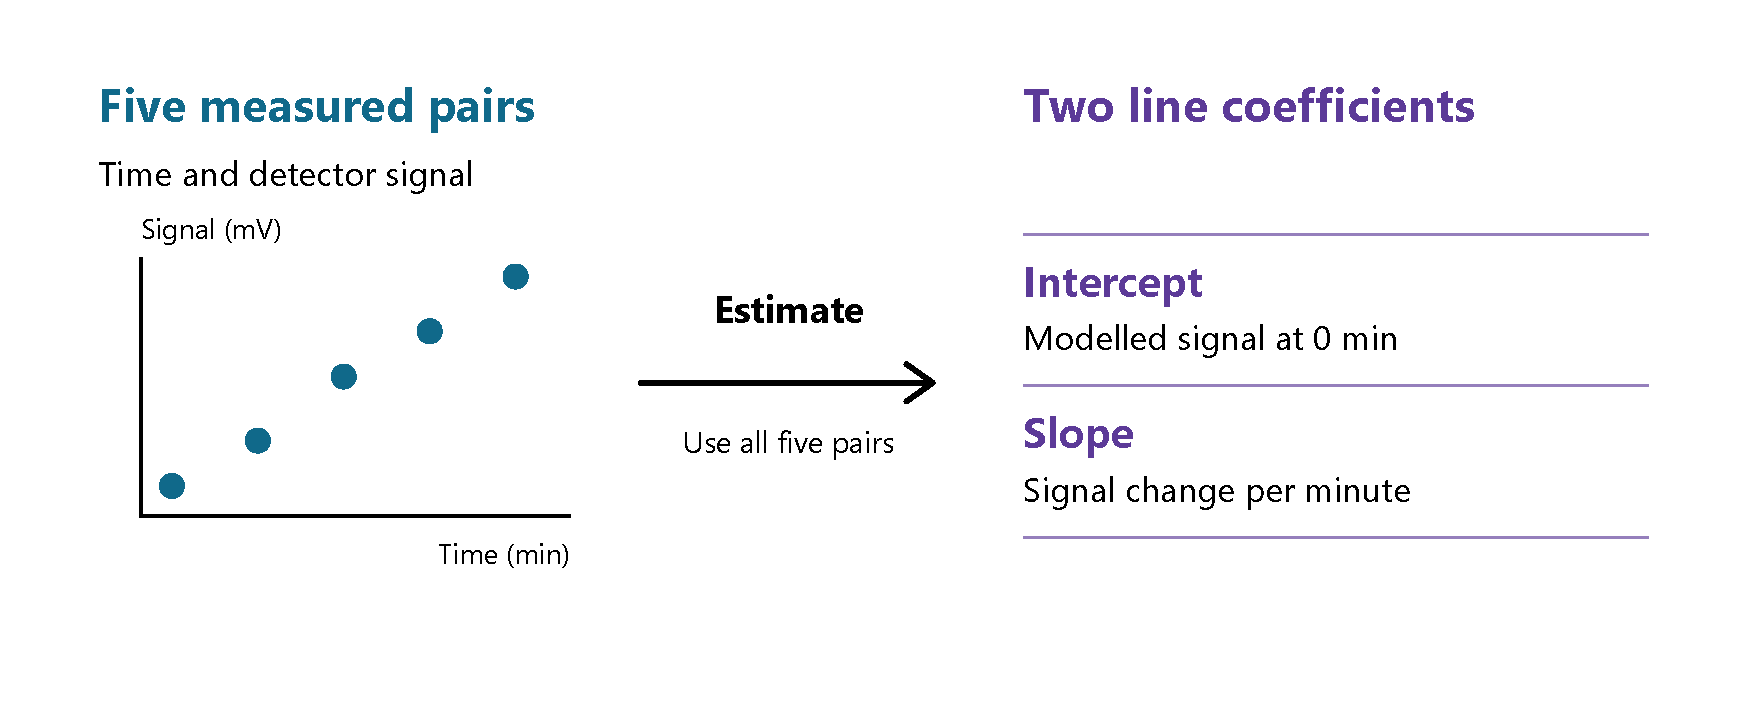
\includegraphics[width=\linewidth,height=.62\textheight,keepaspectratio]{asset-393695d5cf6205fa9cfb9afb288ecd6ebb4cb60a4c53ce268ff0a14cf21ac935.pdf}\end{center}

\medskip

\textbf{Fit by eye: two coefficients}


Try different candidate lines for the same measurements. Change the intercept to raise or lower the line; change the slope to alter its tilt in mV per minute. The manual experiment starts at intercept 0 mV and slope 2.5 mV/min. As you move the sliders, compare the vertical gaps in the scatter plot with the residual bars. A point above the line appears above zero in the residual plot, and a point below the line appears below zero. Ask learners to improve the line and explain which vertical gaps their changes reduce. Do not reveal the fitted coefficient values yet. Compare the visible candidate curve with the fixed observation points; later the normal equations provide a reproducible solution.


\hyperref[material-7c8333ecaf3ab8e47de639679b6cbdcaa5cad8bd8a91cd394f7aa825048275b2]{Fig.~\ref*{material-7c8333ecaf3ab8e47de639679b6cbdcaa5cad8bd8a91cd394f7aa825048275b2}}


\par\medskip
\Needspace{10cm}
\refstepcounter{figure}\label{material-7c8333ecaf3ab8e47de639679b6cbdcaa5cad8bd8a91cd394f7aa825048275b2}
\noindent\textbf{Fig.~\ref*{material-7c8333ecaf3ab8e47de639679b6cbdcaa5cad8bd8a91cd394f7aa825048275b2}.} Fit by eye: two coefficients: formula and complete symbol legend\par\nopagebreak
\begin{center}
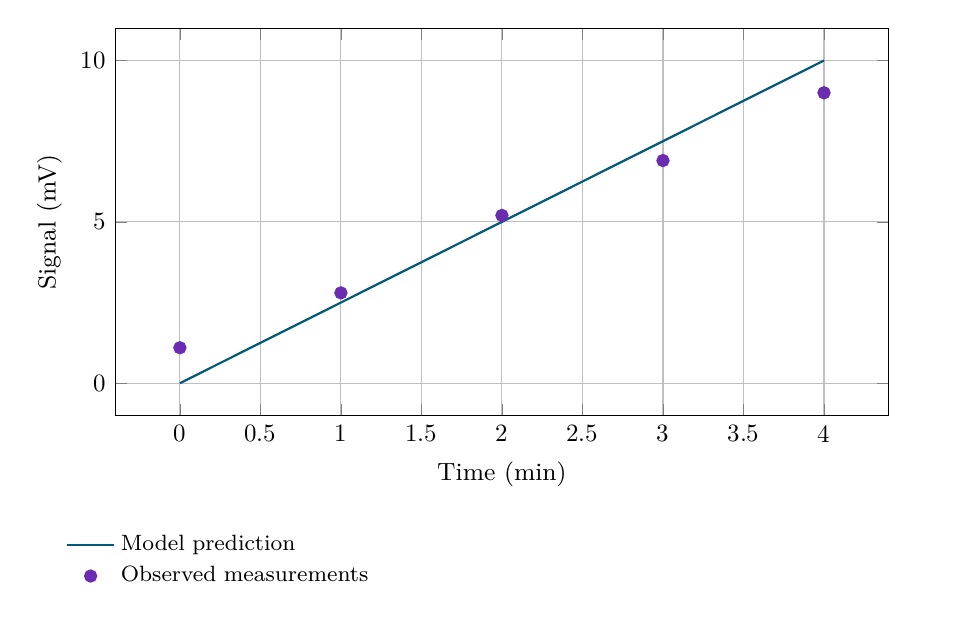
\begin{tikzpicture}
\begin{axis}[width=0.94\linewidth,
height=6.5cm,
scale only axis=false,
grid=major,
tick label style={font=\small},
label style={font=\small},
xlabel={Time (min)},
ylabel={Signal (mV)},
legend style={font=\footnotesize,draw=none,at={(0.5,-0.28)},anchor=north,legend columns=1,text width=0.85\linewidth,align=left},
unbounded coords=jump,
scaled ticks=false,
ymin=-1,
ymax=11]
\addplot[color=pcd1,thick,mark=none] coordinates {(0,0) (0.025,0.0625) (0.05,0.125) (0.075,0.1875) (0.1,0.25) (0.125,0.3125) (0.15,0.375) (0.175,0.4375) (0.2,0.5) (0.225,0.5625) (0.25,0.625) (0.275,0.6875) (0.3,0.75) (0.325,0.8125) (0.35,0.875) (0.375,0.9375) (0.4,1) (0.425,1.0625) (0.45,1.125) (0.475,1.1875) (0.5,1.25) (0.525,1.3125) (0.55,1.375) (0.575,1.4375) (0.6,1.5) (0.625,1.5625) (0.65,1.625) (0.675,1.6875) (0.7,1.75) (0.725,1.8125) (0.75,1.875) (0.775,1.9375) (0.8,2) (0.825,2.0625) (0.85,2.125) (0.875,2.1875) (0.9,2.25) (0.925,2.3125) (0.95,2.375) (0.975,2.4375) (1,2.5) (1.025,2.5625) (1.05,2.625) (1.075,2.6875) (1.1,2.75) (1.125,2.8125) (1.15,2.875) (1.175,2.9375) (1.2,3) (1.225,3.0625) (1.25,3.125) (1.275,3.1875) (1.3,3.25) (1.325,3.3125) (1.35,3.375) (1.375,3.4375) (1.4,3.5) (1.425,3.5625) (1.45,3.625) (1.475,3.6875) (1.5,3.75) (1.525,3.8125) (1.55,3.875) (1.575,3.9375) (1.6,4) (1.625,4.0625) (1.65,4.125) (1.675,4.1875) (1.7,4.25) (1.725,4.3125) (1.75,4.375) (1.775,4.4375) (1.8,4.5) (1.825,4.5625) (1.85,4.625) (1.875,4.6875) (1.9,4.75) (1.925,4.8125) (1.95,4.875) (1.975,4.9375) (2,5) (2.025,5.0625) (2.05,5.125) (2.075,5.1875) (2.1,5.25) (2.125,5.3125) (2.15,5.375) (2.175,5.4375) (2.2,5.5) (2.225,5.5625) (2.25,5.625) (2.275,5.6875) (2.3,5.75) (2.325,5.8125) (2.35,5.875) (2.375,5.9375) (2.4,6) (2.425,6.0625) (2.45,6.125) (2.475,6.1875) (2.5,6.25) (2.525,6.3125) (2.55,6.375) (2.575,6.4375) (2.6,6.5) (2.625,6.5625) (2.65,6.625) (2.675,6.6875) (2.7,6.75) (2.725,6.8125) (2.75,6.875) (2.775,6.9375) (2.8,7) (2.825,7.0625) (2.85,7.125) (2.875,7.1875) (2.9,7.25) (2.925,7.3125) (2.95,7.375) (2.975,7.4375) (3,7.5) (3.025,7.5625) (3.05,7.625) (3.075,7.6875) (3.1,7.75) (3.125,7.8125) (3.15,7.875) (3.175,7.9375) (3.2,8) (3.225,8.0625) (3.25,8.125) (3.275,8.1875) (3.3,8.25) (3.325,8.3125) (3.35,8.375) (3.375,8.4375) (3.4,8.5) (3.425,8.5625) (3.45,8.625) (3.475,8.6875) (3.5,8.75) (3.525,8.8125) (3.55,8.875) (3.575,8.9375) (3.6,9) (3.625,9.0625) (3.65,9.125) (3.675,9.1875) (3.7,9.25) (3.725,9.3125) (3.75,9.375) (3.775,9.4375) (3.8,9.5) (3.825,9.5625) (3.85,9.625) (3.875,9.6875) (3.9,9.75) (3.925,9.8125) (3.95,9.875) (3.975,9.9375) (4,10)};
\addlegendentry{Model prediction}
\addplot[color=pcd2,thick,only marks,mark=*] coordinates {(0,1.1) (1,2.8) (2,5.2) (3,6.9) (4,9)};
\addlegendentry{Observed measurements}

\end{axis}
\end{tikzpicture}
\end{center}

% Full-precision experiment details: {"blockId":"ex:l8-item-04-2--block","parameters":[{"key":"basis","label":"basis","value":0},{"key":"intercept","label":"intercept","value":0},{"key":"slope","label":"slope","value":2.5},{"key":"quadratic","label":"quadratic","value":0},{"key":"mode","label":"mode","value":0},{"key":"showSquaredResiduals","label":"Show sum of squared residuals","value":0},{"key":"signedResidualStages","label":"Reveal the residual plot","value":1}],"readouts":[{"label":"Coefficient b0","value":0},{"label":"Coefficient b1","value":2.5}],"note":"Observation 1: observed 1.1, predicted 0, residual 1.1\nObservation 2: observed 2.8, predicted 2.5, residual 0.2999999999999998\nObservation 3: observed 5.2, predicted 5, residual 0.20000000000000018\nObservation 4: observed 6.9, predicted 7.5, residual -0.5999999999999996\nObservation 5: observed 9, predicted 10, residual -1","markers":[[]]}

\medskip

\hyperref[material-bf34af7c64310a43b3f4a624121791bb67298933993ca431ece8dd90e71ca2e6]{Eq.~\ref*{material-bf34af7c64310a43b3f4a624121791bb67298933993ca431ece8dd90e71ca2e6}}


\par\medskip
\noindent\begin{minipage}{\linewidth}
\refstepcounter{equation}\label{material-bf34af7c64310a43b3f4a624121791bb67298933993ca431ece8dd90e71ca2e6}
\noindent\textbf{Eq.~\ref*{material-bf34af7c64310a43b3f4a624121791bb67298933993ca431ece8dd90e71ca2e6}.} Fit by eye: two coefficients: formula and complete symbol legend\par\nopagebreak
\begin{center}\begin{adjustbox}{max width=\linewidth}$\displaystyle \widehat y_i=\beta_0+\beta_1x_i$\end{adjustbox}\end{center}

\par\noindent\textbf{Symbols}

\par\noindent\textbf{\(+,-,=,\cdot\)} Plus adds, minus subtracts, equals asserts equality; juxtaposition, a centred dot or \ensuremath{\times} between numerical entries multiplies. Parentheses group terms; brackets arrange matrix entries. Bare numerical constants are dimensionless unless the stated measurement coordinates give units.

\par\noindent\textbf{\(\beta_0\)} Candidate intercept, in mV; a fitted coefficient is marked with a hat.

\par\noindent\textbf{\(\beta_1\)} Candidate slope, in mV/min; a fitted coefficient is marked with a hat.

\par\noindent\textbf{\(\widehat y_i\)} Fitted signal for observation i, in mV; the hat denotes a fitted value, not an additional observation.

\par\noindent\textbf{\(i,n\)} Observation index i runs from 1 to n; here n = 5, in increasing time order.

\par\noindent\textbf{\(x_i\)} Time for observation i, in min; the unindexed x is a selected time in the same unit.

\end{minipage}\par
\medskip

\textbf{Give every vertical gap a sign}


Use the adjustable candidate line in \hyperref[material-7c8333ecaf3ab8e47de639679b6cbdcaa5cad8bd8a91cd394f7aa825048275b2]{Fig.~\ref*{material-7c8333ecaf3ab8e47de639679b6cbdcaa5cad8bd8a91cd394f7aa825048275b2}} to connect the scatter plot with the residual bars. Compute each observation minus its prediction at exactly the same time. A point above the line has positive residual; one below has negative residual. Move the sliders and check how the signed residuals change. These are vertical signal gaps, not perpendicular geometric distances.


\textbf{What happens when we add the signed gaps?}


Adding the five residuals gives 0.00 mV. Each point still misses the fitted line: positive and negative gaps cancel. The next step is to define a score that counts gaps on both sides.
\textbf{What should we minimise to fit a line?}


The comparison figure uses the same five measurements for two candidate lines. The starting line has intercept 0 mV and slope 2.5 mV/min, with residuals +1.10, +0.30, +0.20, \ensuremath{-}0.60 and \ensuremath{-}1.00 mV. The other line has intercept 1 mV and slope 2 mV/min, with residuals +0.10, \ensuremath{-}0.20, +0.20, \ensuremath{-}0.10 and 0.00 mV. Both signed sums are zero. Squaring the residuals before adding gives 2.70 mV\ensuremath{{}^2} for the first line and 0.10 mV\ensuremath{{}^2} for the second. A gap twice as large contributes four times as much. Absolute deviations would also prevent cancellation. The squared score is differentiable in the coefficients, which is useful when we derive the normal equations.


\hyperref[material-8dd6b53793fd81f55643ef230d898b3913765799c0d3d219216d5c7fb3907808]{Fig.~\ref*{material-8dd6b53793fd81f55643ef230d898b3913765799c0d3d219216d5c7fb3907808}}


\par\medskip
\Needspace{10cm}
\refstepcounter{figure}\label{material-8dd6b53793fd81f55643ef230d898b3913765799c0d3d219216d5c7fb3907808}
\noindent\textbf{Fig.~\ref*{material-8dd6b53793fd81f55643ef230d898b3913765799c0d3d219216d5c7fb3907808}.} What should we minimise to fit a line? Comparing residual scores\par\nopagebreak
\begin{center}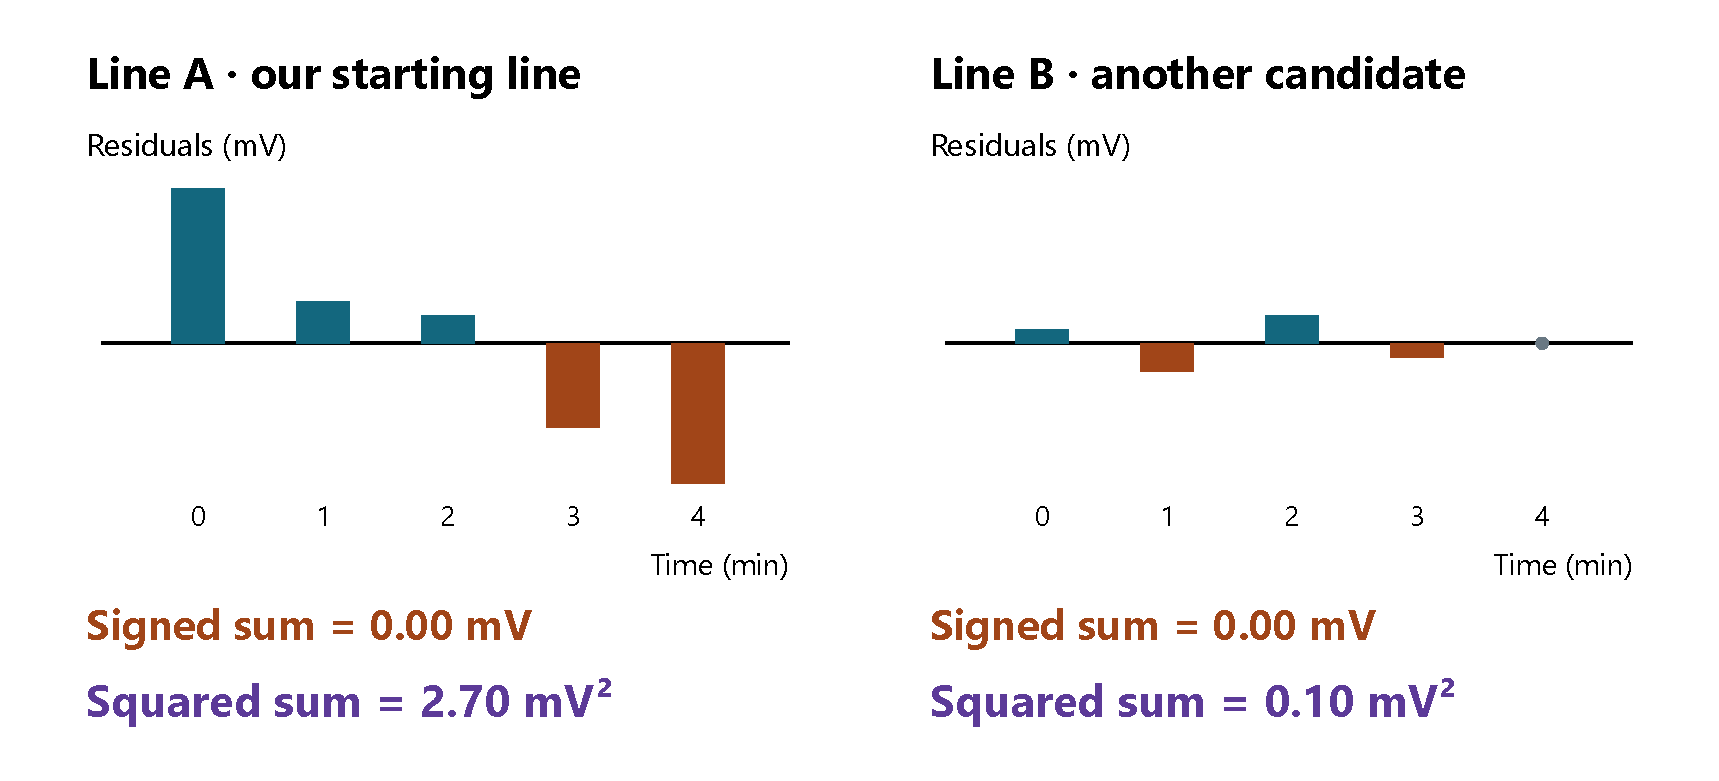
\includegraphics[width=\linewidth,height=.62\textheight,keepaspectratio]{asset-972f224ecf0b04263109bfd00b3d001b4e607e1f3541e9cee01bc74203330a4c.pdf}\end{center}

\medskip

\hyperref[material-bcf06d3656a8adcb9ae629a5324795c47e739577357d8e0aeea62ff68698b6b2]{Eq.~\ref*{material-bcf06d3656a8adcb9ae629a5324795c47e739577357d8e0aeea62ff68698b6b2}}


\par\medskip
\noindent\begin{minipage}{\linewidth}
\refstepcounter{equation}\label{material-bcf06d3656a8adcb9ae629a5324795c47e739577357d8e0aeea62ff68698b6b2}
\noindent\textbf{Eq.~\ref*{material-bcf06d3656a8adcb9ae629a5324795c47e739577357d8e0aeea62ff68698b6b2}.} Least-squares objective and symbol legend\par\nopagebreak
\begin{center}\begin{adjustbox}{max width=\linewidth}$\displaystyle Q(\beta_0,\beta_1)=\sum_{i=1}^{n}[y_i-(\beta_0+\beta_1x_i)]^2$\end{adjustbox}\end{center}

\par\noindent\textbf{Symbols}

\par\noindent\textbf{\(({\cdot})^2\)} Square the complete enclosed value; squared signal residuals have unit mV\ensuremath{{}^2}.

\par\noindent\textbf{\(+,-,=,\cdot\)} Plus adds, minus subtracts, equals asserts equality; juxtaposition, a centred dot or \ensuremath{\times} between numerical entries multiplies. Parentheses group terms; brackets arrange matrix entries. Bare numerical constants are dimensionless unless the stated measurement coordinates give units.

\par\noindent\textbf{\(Q,\mathrm{SSE}\)} Q is the candidate sum of squared residuals; SSE is its value at the fitted coefficients, in mV\ensuremath{{}^2}.

\par\noindent\textbf{\(\beta_0\)} Candidate intercept, in mV; a fitted coefficient is marked with a hat.

\par\noindent\textbf{\(\beta_1\)} Candidate slope, in mV/min; a fitted coefficient is marked with a hat.

\par\noindent\textbf{\(\sum_{i=1}^{n}\)} Add one term for each observation i from 1 through n.

\par\noindent\textbf{\(i,n\)} Observation index i runs from 1 to n; here n = 5, in increasing time order.

\par\noindent\textbf{\(x_i\)} Time for observation i, in min; the unindexed x is a selected time in the same unit.

\par\noindent\textbf{\(y_i\)} Observed signal for observation i, in mV; y is the column of all five signals.

\end{minipage}\par
\medskip

\textbf{Where is the squared error smallest?}


With the observations fixed, try changing one coefficient at a time. Each local error plot shows a slice of the squared-error surface near the corresponding slider setting. The other coefficient is held at its current value. Both plots mark the same current squared error. The total differential gives the first-order change in squared error for a change in both coefficients. At the joint minimum it is zero for every direction. We can vary one coefficient while keeping the other fixed. Doing this for each coefficient shows that both partial derivatives must be zero at the same pair of values. For these data, the quadratic curves upward and the pair is unique. To find the pair we need to solve the two equations together. Matrix notation gives us a compact way to do that.


\hyperref[material-b6f410122e6a4a1138201c1189b7236a61b0fb25e658ca3c23b452b3b1265fab]{Fig.~\ref*{material-b6f410122e6a4a1138201c1189b7236a61b0fb25e658ca3c23b452b3b1265fab}}


\par\medskip
\Needspace{10cm}
\refstepcounter{figure}\label{material-b6f410122e6a4a1138201c1189b7236a61b0fb25e658ca3c23b452b3b1265fab}
\noindent\textbf{Fig.~\ref*{material-b6f410122e6a4a1138201c1189b7236a61b0fb25e658ca3c23b452b3b1265fab}.} Local views of squared error with adjustable coefficients\par\nopagebreak
\begin{center}
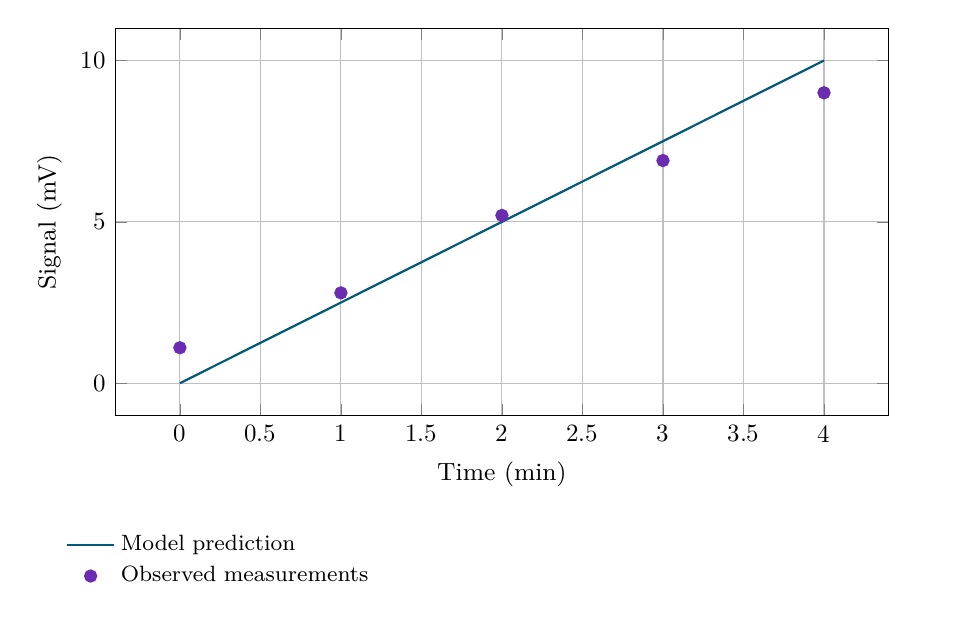
\begin{tikzpicture}
\begin{axis}[width=0.94\linewidth,
height=6.5cm,
scale only axis=false,
grid=major,
tick label style={font=\small},
label style={font=\small},
xlabel={Time (min)},
ylabel={Signal (mV)},
legend style={font=\footnotesize,draw=none,at={(0.5,-0.28)},anchor=north,legend columns=1,text width=0.85\linewidth,align=left},
unbounded coords=jump,
scaled ticks=false,
ymin=-1,
ymax=11]
\addplot[color=pcd1,thick,mark=none] coordinates {(0,0) (0.025,0.0625) (0.05,0.125) (0.075,0.1875) (0.1,0.25) (0.125,0.3125) (0.15,0.375) (0.175,0.4375) (0.2,0.5) (0.225,0.5625) (0.25,0.625) (0.275,0.6875) (0.3,0.75) (0.325,0.8125) (0.35,0.875) (0.375,0.9375) (0.4,1) (0.425,1.0625) (0.45,1.125) (0.475,1.1875) (0.5,1.25) (0.525,1.3125) (0.55,1.375) (0.575,1.4375) (0.6,1.5) (0.625,1.5625) (0.65,1.625) (0.675,1.6875) (0.7,1.75) (0.725,1.8125) (0.75,1.875) (0.775,1.9375) (0.8,2) (0.825,2.0625) (0.85,2.125) (0.875,2.1875) (0.9,2.25) (0.925,2.3125) (0.95,2.375) (0.975,2.4375) (1,2.5) (1.025,2.5625) (1.05,2.625) (1.075,2.6875) (1.1,2.75) (1.125,2.8125) (1.15,2.875) (1.175,2.9375) (1.2,3) (1.225,3.0625) (1.25,3.125) (1.275,3.1875) (1.3,3.25) (1.325,3.3125) (1.35,3.375) (1.375,3.4375) (1.4,3.5) (1.425,3.5625) (1.45,3.625) (1.475,3.6875) (1.5,3.75) (1.525,3.8125) (1.55,3.875) (1.575,3.9375) (1.6,4) (1.625,4.0625) (1.65,4.125) (1.675,4.1875) (1.7,4.25) (1.725,4.3125) (1.75,4.375) (1.775,4.4375) (1.8,4.5) (1.825,4.5625) (1.85,4.625) (1.875,4.6875) (1.9,4.75) (1.925,4.8125) (1.95,4.875) (1.975,4.9375) (2,5) (2.025,5.0625) (2.05,5.125) (2.075,5.1875) (2.1,5.25) (2.125,5.3125) (2.15,5.375) (2.175,5.4375) (2.2,5.5) (2.225,5.5625) (2.25,5.625) (2.275,5.6875) (2.3,5.75) (2.325,5.8125) (2.35,5.875) (2.375,5.9375) (2.4,6) (2.425,6.0625) (2.45,6.125) (2.475,6.1875) (2.5,6.25) (2.525,6.3125) (2.55,6.375) (2.575,6.4375) (2.6,6.5) (2.625,6.5625) (2.65,6.625) (2.675,6.6875) (2.7,6.75) (2.725,6.8125) (2.75,6.875) (2.775,6.9375) (2.8,7) (2.825,7.0625) (2.85,7.125) (2.875,7.1875) (2.9,7.25) (2.925,7.3125) (2.95,7.375) (2.975,7.4375) (3,7.5) (3.025,7.5625) (3.05,7.625) (3.075,7.6875) (3.1,7.75) (3.125,7.8125) (3.15,7.875) (3.175,7.9375) (3.2,8) (3.225,8.0625) (3.25,8.125) (3.275,8.1875) (3.3,8.25) (3.325,8.3125) (3.35,8.375) (3.375,8.4375) (3.4,8.5) (3.425,8.5625) (3.45,8.625) (3.475,8.6875) (3.5,8.75) (3.525,8.8125) (3.55,8.875) (3.575,8.9375) (3.6,9) (3.625,9.0625) (3.65,9.125) (3.675,9.1875) (3.7,9.25) (3.725,9.3125) (3.75,9.375) (3.775,9.4375) (3.8,9.5) (3.825,9.5625) (3.85,9.625) (3.875,9.6875) (3.9,9.75) (3.925,9.8125) (3.95,9.875) (3.975,9.9375) (4,10)};
\addlegendentry{Model prediction}
\addplot[color=pcd2,thick,only marks,mark=*] coordinates {(0,1.1) (1,2.8) (2,5.2) (3,6.9) (4,9)};
\addlegendentry{Observed measurements}

\end{axis}
\end{tikzpicture}
\end{center}

% Full-precision experiment details: {"blockId":"ex:l8-minimum-two-coefficients-item-2--block","parameters":[{"key":"basis","label":"basis","value":0},{"key":"intercept","label":"intercept","value":0},{"key":"slope","label":"slope","value":2.5},{"key":"quadratic","label":"quadratic","value":0},{"key":"mode","label":"mode","value":0},{"key":"localSquaredErrorPlots","label":"Show local squared-error plots","value":1}],"readouts":[{"label":"Coefficient b0","value":0},{"label":"Coefficient b1","value":2.5},{"label":"Sum of squared residuals","value":2.6999999999999997}],"note":"Observation 1: observed 1.1, predicted 0, residual 1.1\nObservation 2: observed 2.8, predicted 2.5, residual 0.2999999999999998\nObservation 3: observed 5.2, predicted 5, residual 0.20000000000000018\nObservation 4: observed 6.9, predicted 7.5, residual -0.5999999999999996\nObservation 5: observed 9, predicted 10, residual -1","markers":[[]]}

\medskip

\hyperref[material-b6541617aa1e4fe891255a35da265647de78be61b206de739b8b8b6d25435383]{Eq.~\ref*{material-b6541617aa1e4fe891255a35da265647de78be61b206de739b8b8b6d25435383}}


\par\medskip
\noindent\begin{minipage}{\linewidth}
\refstepcounter{equation}\label{material-b6541617aa1e4fe891255a35da265647de78be61b206de739b8b8b6d25435383}
\noindent\textbf{Eq.~\ref*{material-b6541617aa1e4fe891255a35da265647de78be61b206de739b8b8b6d25435383}.} Squared error, total differential and minimum conditions\par\nopagebreak
\begin{center}\begin{adjustbox}{max width=\linewidth}$\displaystyle \begin{aligned}Q(\beta_0,\beta_1)&=\sum_{i=1}^{n}[y_i-\beta_0-\beta_1 x_i]^2\\[.45em]\mathrm dQ&=\frac{\partial Q}{\partial\beta_0}\,\mathrm d\beta_0+\frac{\partial Q}{\partial\beta_1}\,\mathrm d\beta_1\\[.45em]\frac{\partial Q}{\partial\beta_0}&=0,\qquad \frac{\partial Q}{\partial\beta_1}=0\end{aligned}$\end{adjustbox}\end{center}

\par\noindent\textbf{Symbols}

\par\noindent\textbf{\(({\cdot})^2\)} Square the complete enclosed value; squared signal residuals have unit mV\ensuremath{{}^2}.

\par\noindent\textbf{\(+,-,=,\cdot\)} Plus adds, minus subtracts, equals asserts equality; juxtaposition, a centred dot or \ensuremath{\times} between numerical entries multiplies. Parentheses group terms; brackets arrange matrix entries. Bare numerical constants are dimensionless unless the stated measurement coordinates give units.

\par\noindent\textbf{\(0\)} Zero scalar or zero column as dictated by shape. In X\ensuremath{{}^{\mathsf T}}e the two components have units mV and min\ensuremath{\cdot}mV, and each equals zero in its own unit.

\par\noindent\textbf{\(Q,\mathrm{SSE}\)} Q is the candidate sum of squared residuals; SSE is its value at the fitted coefficients, in mV\ensuremath{{}^2}.

\par\noindent\textbf{\(\beta_0\)} Candidate intercept, in mV; a fitted coefficient is marked with a hat.

\par\noindent\textbf{\(\beta_1\)} Candidate slope, in mV/min; a fitted coefficient is marked with a hat.

\par\noindent\textbf{\(\mathrm dQ,\ \mathrm d\beta_0,\ \mathrm d\beta_1\)} First-order change in Q and the two independent coefficient increments. Their units here are mV\ensuremath{{}^2}, mV and mV/min, respectively.

\par\noindent\textbf{\(\partial,\frac{d}{da}\)} Partial differentiation changes one coefficient while holding other coefficients and all data fixed; d/da is the ordinary scalar derivative with respect to a.

\par\noindent\textbf{\(\sum_{i=1}^{n}\)} Add one term for each observation i from 1 through n.

\par\noindent\textbf{\(x_i\)} Time for observation i, in min; the unindexed x is a selected time in the same unit.

\par\noindent\textbf{\(y_i\)} Observed signal for observation i, in mV; y is the column of all five signals.

\end{minipage}\par
\medskip

\clearpage
\section{Matrix algebra and simultaneous equations}
\textbf{Matrix Algebra}


This short detour introduces the operations we will use to express the two regression conditions together.


\textbf{Matrix Shapes: count rows before columns}


Compare the 2 by 3, 3 by 2 and 2 by 4 arrays. Count horizontal rows first and vertical columns second. The first two arrays contain the same number of entries, but their shapes differ.


\hyperref[material-41ab0f26f3d226a89887dd5d23928dc286e316eeedb84ed1779563ac3b36146c]{Eq.~\ref*{material-41ab0f26f3d226a89887dd5d23928dc286e316eeedb84ed1779563ac3b36146c}}


\par\medskip
\noindent\begin{minipage}{\linewidth}
\refstepcounter{equation}\label{material-41ab0f26f3d226a89887dd5d23928dc286e316eeedb84ed1779563ac3b36146c}
\noindent\textbf{Eq.~\ref*{material-41ab0f26f3d226a89887dd5d23928dc286e316eeedb84ed1779563ac3b36146c}.} Matrix Shapes: count rows before columns: formula and complete symbol legend\par\nopagebreak
\begin{center}\begin{adjustbox}{max width=\linewidth}$\displaystyle \underbrace{\begin{bmatrix}1&2&3\\4&5&6\end{bmatrix}}_{2\times3}\qquad\underbrace{\begin{bmatrix}2&5\\4&7\\1&3\end{bmatrix}}_{3\times2}\qquad\underbrace{\begin{bmatrix}3&0&-1&4\\2&6&5&1\end{bmatrix}}_{2\times4}$\end{adjustbox}\end{center}

\par\noindent\textbf{Symbols}

\par\noindent\textbf{\(+,-,=,\cdot\)} Plus adds, minus subtracts, equals asserts equality; juxtaposition, a centred dot or \ensuremath{\times} between numerical entries multiplies. Parentheses group terms; brackets arrange matrix entries. Bare numerical constants are dimensionless unless the stated measurement coordinates give units.

\par\noindent\textbf{\(A,B\)} Named numerical matrices; entries in the matrix examples are dimensionless. Matrix juxtaposition denotes row-by-column multiplication, not entrywise multiplication.

\par\noindent\textbf{\(\in,\mathbb R\)} \ensuremath{\in} means belongs to; \ensuremath{\mathbb{R}} denotes real numbers; \ensuremath{\mathbb{R}}\textasciicircum{}(m\ensuremath{\times}n) is the set of real m-row, n-column matrices.

\par\noindent\textbf{\(m,n,p\)} Positive integer row, inner and column counts. In a shape m \ensuremath{\times} n, the first count is rows and the second columns; \ensuremath{\times} here separates dimensions.

\end{minipage}\par
\medskip

\textbf{Matrix Indexing: row first, then column}


Read a subscript pair in a fixed order. In the shown matrix, a subscript 23 means row 2 then column 3, so its value is 6. It does not mean row 3 column 2, and it does not mean the number twenty-three. The box marks that matrix entry.


\hyperref[material-873ef499a03ec6b6bb8c4f209ef86a34083e3ac8efd7859d1ce5b08284e6ebbe]{Eq.~\ref*{material-873ef499a03ec6b6bb8c4f209ef86a34083e3ac8efd7859d1ce5b08284e6ebbe}}


\par\medskip
\noindent\begin{minipage}{\linewidth}
\refstepcounter{equation}\label{material-873ef499a03ec6b6bb8c4f209ef86a34083e3ac8efd7859d1ce5b08284e6ebbe}
\noindent\textbf{Eq.~\ref*{material-873ef499a03ec6b6bb8c4f209ef86a34083e3ac8efd7859d1ce5b08284e6ebbe}.} Matrix Indexing: row first, then column – formula and complete symbol legend\par\nopagebreak
\begin{center}\begin{adjustbox}{max width=\linewidth}$\displaystyle A=\begin{bmatrix}1&2&3\\4&5&\boxed{6}\end{bmatrix},\qquad a_{23}=\boxed{6}$\end{adjustbox}\end{center}

\par\noindent\textbf{Symbols}

\par\noindent\textbf{\(+,-,=,\cdot\)} Plus adds, minus subtracts, equals asserts equality; juxtaposition, a centred dot or \ensuremath{\times} between numerical entries multiplies. Parentheses group terms; brackets arrange matrix entries. Bare numerical constants are dimensionless unless the stated measurement coordinates give units.

\par\noindent\textbf{\(A,B\)} Named numerical matrices; entries in the matrix examples are dimensionless. Matrix juxtaposition denotes row-by-column multiplication, not entrywise multiplication.

\par\noindent\textbf{\(a_{ij}\)} Entry of A in row i and column j. The first subscript is always the row; indices begin at 1.

\par\noindent\textbf{\(i,j,k\)} Row index i, column index j, and inner-product index k; each runs over the valid rows/columns indicated by the matrix shape.

\end{minipage}\par
\medskip

\textbf{Matrix Types: square matrices}


Compare the 2 by 2, 3 by 3 and 4 by 4 examples. Every one is square because its row and column counts match. The positions and values of the entries can vary.


\hyperref[material-e3c84a6f43b7c6650a3c62b36d088a1337c72610ee8d96402ca6853e7e212e4e]{Eq.~\ref*{material-e3c84a6f43b7c6650a3c62b36d088a1337c72610ee8d96402ca6853e7e212e4e}}


\par\medskip
\noindent\begin{minipage}{\linewidth}
\refstepcounter{equation}\label{material-e3c84a6f43b7c6650a3c62b36d088a1337c72610ee8d96402ca6853e7e212e4e}
\noindent\textbf{Eq.~\ref*{material-e3c84a6f43b7c6650a3c62b36d088a1337c72610ee8d96402ca6853e7e212e4e}.} Matrix Types: square matrices – formula and complete symbol legend\par\nopagebreak
\begin{center}\begin{adjustbox}{max width=\linewidth}$\displaystyle \underbrace{\begin{bmatrix}1&2\\3&4\end{bmatrix}}_{2\times2}\qquad\underbrace{\begin{bmatrix}2&1&0\\3&4&2\\1&5&6\end{bmatrix}}_{3\times3}\qquad\underbrace{\begin{bmatrix}2&0&3&1\\4&1&0&2\\5&3&2&0\\1&0&6&4\end{bmatrix}}_{4\times4}$\end{adjustbox}\end{center}

\par\noindent\textbf{Symbols}

\par\noindent\textbf{\(+,-,=,\cdot\)} Plus adds, minus subtracts, equals asserts equality; juxtaposition, a centred dot or \ensuremath{\times} between numerical entries multiplies. Parentheses group terms; brackets arrange matrix entries. Bare numerical constants are dimensionless unless the stated measurement coordinates give units.

\par\noindent\textbf{\(A,B\)} Named numerical matrices; entries in the matrix examples are dimensionless. Matrix juxtaposition denotes row-by-column multiplication, not entrywise multiplication.

\end{minipage}\par
\medskip

\textbf{Matrix Types: diagonal matrices}


Compare diagonal matrices of sizes 2, 3 and 4. The highlighted diagonal is where the row and column indices agree. Every off-diagonal entry is zero. The 3 by 3 example has a zero on its main diagonal, which makes it singular.


\hyperref[material-d1cf98ea4ce87e23be9e5cbd9aa3529951adab2bc6399bae275c299ad2302b76]{Eq.~\ref*{material-d1cf98ea4ce87e23be9e5cbd9aa3529951adab2bc6399bae275c299ad2302b76}}


\par\medskip
\noindent\begin{minipage}{\linewidth}
\refstepcounter{equation}\label{material-d1cf98ea4ce87e23be9e5cbd9aa3529951adab2bc6399bae275c299ad2302b76}
\noindent\textbf{Eq.~\ref*{material-d1cf98ea4ce87e23be9e5cbd9aa3529951adab2bc6399bae275c299ad2302b76}.} Matrix Types: diagonal matrices – formula and complete symbol legend\par\nopagebreak
\begin{center}\begin{adjustbox}{max width=\linewidth}$\displaystyle \underbrace{\begin{bmatrix}\boxed{2}&0\\0&\boxed{3}\end{bmatrix}}_{2\times2}\qquad\underbrace{\begin{bmatrix}\boxed{4}&0&0\\0&\boxed{0}&0\\0&0&\boxed{-2}\end{bmatrix}}_{3\times3}\qquad\underbrace{\begin{bmatrix}\boxed{3}&0&0&0\\0&\boxed{-1}&0&0\\0&0&\boxed{5}&0\\0&0&0&\boxed{2}\end{bmatrix}}_{4\times4}$\end{adjustbox}\end{center}

\par\noindent\textbf{Symbols}

\par\noindent\textbf{\(+,-,=,\cdot\)} Plus adds, minus subtracts, equals asserts equality; juxtaposition, a centred dot or \ensuremath{\times} between numerical entries multiplies. Parentheses group terms; brackets arrange matrix entries. Bare numerical constants are dimensionless unless the stated measurement coordinates give units.

\par\noindent\textbf{\(D\)} Diagonal square matrix: entries off the main diagonal are zero; diagonal entries need not equal one.

\end{minipage}\par
\medskip

\textbf{Matrix Types: identity matrices}


Compare the identities of sizes 1, 2 and 3. Every diagonal entry is one. The left identity for a 2 by 3 matrix must have size 2, and the right identity must have size 3. Both products preserve the same matrix A.


\hyperref[material-16121827aec21dc56c4feefbec0ad8fc4019f012363014545704d93c34874cfd]{Eq.~\ref*{material-16121827aec21dc56c4feefbec0ad8fc4019f012363014545704d93c34874cfd}}


\par\medskip
\noindent\begin{minipage}{\linewidth}
\refstepcounter{equation}\label{material-16121827aec21dc56c4feefbec0ad8fc4019f012363014545704d93c34874cfd}
\noindent\textbf{Eq.~\ref*{material-16121827aec21dc56c4feefbec0ad8fc4019f012363014545704d93c34874cfd}.} Matrix Types: identity matrices – formula and complete symbol legend\par\nopagebreak
\begin{center}\begin{adjustbox}{max width=\linewidth}$\displaystyle \begin{gathered}I_1=\begin{bmatrix}\boxed{1}\end{bmatrix}\qquad I_2=\begin{bmatrix}\boxed{1}&0\\0&\boxed{1}\end{bmatrix}\qquad I_3=\begin{bmatrix}\boxed{1}&0&0\\0&\boxed{1}&0\\0&0&\boxed{1}\end{bmatrix}\\[.5em]AI_3=I_2A=A\qquad\text{for a } 2\times3\ \text{matrix } A\end{gathered}$\end{adjustbox}\end{center}

\par\noindent\textbf{Symbols}

\par\noindent\textbf{\(+,-,=,\cdot\)} Plus adds, minus subtracts, equals asserts equality; juxtaposition, a centred dot or \ensuremath{\times} between numerical entries multiplies. Parentheses group terms; brackets arrange matrix entries. Bare numerical constants are dimensionless unless the stated measurement coordinates give units.

\par\noindent\textbf{\(A,B\)} Named numerical matrices; entries in the matrix examples are dimensionless. Matrix juxtaposition denotes row-by-column multiplication, not entrywise multiplication.

\par\noindent\textbf{\(I\)} Identity matrix of the required square size: ones on the main diagonal, zeros elsewhere. Multiplication by I leaves a compatible matrix unchanged.

\end{minipage}\par
\medskip

\textbf{Matrix Arithmetic: addition and subtraction}


Both matrices have the same shape. Read the top-left cells first: add 1 and 5 or subtract 5 from 1. Then do the same at each of the other three positions. The result keeps the original shape. When entries have units, the two values being combined must have compatible units.


\hyperref[material-0d2f8faee1b5ba5cfccf8a0204bbaa3871d54d486fe38574649f7e6c68e2fa94]{Eq.~\ref*{material-0d2f8faee1b5ba5cfccf8a0204bbaa3871d54d486fe38574649f7e6c68e2fa94}}


\par\medskip
\noindent\begin{minipage}{\linewidth}
\refstepcounter{equation}\label{material-0d2f8faee1b5ba5cfccf8a0204bbaa3871d54d486fe38574649f7e6c68e2fa94}
\noindent\textbf{Eq.~\ref*{material-0d2f8faee1b5ba5cfccf8a0204bbaa3871d54d486fe38574649f7e6c68e2fa94}.} Matrix Arithmetic: addition and subtraction – formula and complete symbol legend\par\nopagebreak
\begin{center}\begin{adjustbox}{max width=\linewidth}$\displaystyle \begin{aligned}A&=\begin{bmatrix}1&2\\3&4\end{bmatrix},\qquad B=\begin{bmatrix}5&6\\7&8\end{bmatrix}\\A+B&=\begin{bmatrix}\boxed{1+5}&2+6\\3+7&4+8\end{bmatrix}=\begin{bmatrix}6&8\\10&12\end{bmatrix}\\A-B&=\begin{bmatrix}\boxed{1-5}&2-6\\3-7&4-8\end{bmatrix}=\begin{bmatrix}-4&-4\\-4&-4\end{bmatrix}\end{aligned}$\end{adjustbox}\end{center}

\par\noindent\textbf{Symbols}

\par\noindent\textbf{\(+,-,=,\cdot\)} Plus adds, minus subtracts, equals asserts equality; juxtaposition, a centred dot or \ensuremath{\times} between numerical entries multiplies. Parentheses group terms; brackets arrange matrix entries. Bare numerical constants are dimensionless unless the stated measurement coordinates give units.

\par\noindent\textbf{\(A,B\)} Named numerical matrices; entries in the matrix examples are dimensionless. Matrix juxtaposition denotes row-by-column multiplication, not entrywise multiplication.

\end{minipage}\par
\medskip

\textbf{Matrix Arithmetic: multiplication by a scalar}


Multiply each entry by the same scalar. The first calculation multiplies 1 by 2, and the remaining cells repeat the same operation with 2, 3 and 4. The positions and the shape stay the same. A dimensionless scalar preserves the units of the entries.


\hyperref[material-06c59fb1c85cb32d874556571e51748179be01a558054d8d289b088ddf649e01]{Eq.~\ref*{material-06c59fb1c85cb32d874556571e51748179be01a558054d8d289b088ddf649e01}}


\par\medskip
\noindent\begin{minipage}{\linewidth}
\refstepcounter{equation}\label{material-06c59fb1c85cb32d874556571e51748179be01a558054d8d289b088ddf649e01}
\noindent\textbf{Eq.~\ref*{material-06c59fb1c85cb32d874556571e51748179be01a558054d8d289b088ddf649e01}.} Matrix Arithmetic: multiplication by a scalar – formula and complete symbol legend\par\nopagebreak
\begin{center}\begin{adjustbox}{max width=\linewidth}$\displaystyle \begin{aligned}2\begin{bmatrix}1&2\\3&4\end{bmatrix}&=\begin{bmatrix}\boxed{2\cdot1}&2\cdot2\\2\cdot3&2\cdot4\end{bmatrix}\\&=\begin{bmatrix}2&4\\6&8\end{bmatrix}\end{aligned}$\end{adjustbox}\end{center}

\par\noindent\textbf{Symbols}

\par\noindent\textbf{\(+,-,=,\cdot\)} Plus adds, minus subtracts, equals asserts equality; juxtaposition, a centred dot or \ensuremath{\times} between numerical entries multiplies. Parentheses group terms; brackets arrange matrix entries. Bare numerical constants are dimensionless unless the stated measurement coordinates give units.

\par\noindent\textbf{\(c\)} A dimensionless scalar; cA multiplies every entry of A by c.

\end{minipage}\par
\medskip

\textbf{Matrix Transpose: rows become columns}


The first row [1,2,3] becomes the first column and the second row [4,5,6] becomes the second column. Shape two-by-three therefore becomes three-by-two. Transposing twice returns the original matrix. Later X transpose will collect dot products with the columns of X.


\hyperref[material-2d1007cbc554039138cb37233ce80d3c02f64dc19c57db16c302becd25605ef9]{Eq.~\ref*{material-2d1007cbc554039138cb37233ce80d3c02f64dc19c57db16c302becd25605ef9}}


\par\medskip
\noindent\begin{minipage}{\linewidth}
\refstepcounter{equation}\label{material-2d1007cbc554039138cb37233ce80d3c02f64dc19c57db16c302becd25605ef9}
\noindent\textbf{Eq.~\ref*{material-2d1007cbc554039138cb37233ce80d3c02f64dc19c57db16c302becd25605ef9}.} Matrix Transpose: rows become columns – formula and complete symbol legend\par\nopagebreak
\begin{center}\begin{adjustbox}{max width=\linewidth}$\displaystyle \begin{bmatrix}\boxed{1}&\boxed{2}&\boxed{3}\\4&5&6\end{bmatrix}^{\mathsf T}=\begin{bmatrix}\boxed{1}&4\\\boxed{2}&5\\\boxed{3}&6\end{bmatrix}$\end{adjustbox}\end{center}

\par\noindent\textbf{Symbols}

\par\noindent\textbf{\(+,-,=,\cdot\)} Plus adds, minus subtracts, equals asserts equality; juxtaposition, a centred dot or \ensuremath{\times} between numerical entries multiplies. Parentheses group terms; brackets arrange matrix entries. Bare numerical constants are dimensionless unless the stated measurement coordinates give units.

\par\noindent\textbf{\({}^{\mathsf T}\)} Transpose: swap rows and columns. (AB)\ensuremath{{}^{\mathsf T}} reverses the multiplication order to B\ensuremath{{}^{\mathsf T}}A\ensuremath{{}^{\mathsf T}}.

\end{minipage}\par
\medskip

\textbf{Matrix Multiplication: which dimensions must match?}


A matrix with m rows and n columns can multiply one with n rows and p columns. Each output entry needs a complete row and a complete column of equal length. The result has m rows and p columns. As a quick question, a two-by-three times a three-by-four is valid and yields two-by-four; the reverse order is not valid. Pause for the shape answer before continuing.


\hyperref[material-c697330e97a68807a97b0927b1eba4c8aa87a24b7b090e7a0e31c24889e3586a]{Eq.~\ref*{material-c697330e97a68807a97b0927b1eba4c8aa87a24b7b090e7a0e31c24889e3586a}}


\par\medskip
\noindent\begin{minipage}{\linewidth}
\refstepcounter{equation}\label{material-c697330e97a68807a97b0927b1eba4c8aa87a24b7b090e7a0e31c24889e3586a}
\noindent\textbf{Eq.~\ref*{material-c697330e97a68807a97b0927b1eba4c8aa87a24b7b090e7a0e31c24889e3586a}.} Matrix Multiplication: which dimensions must match? – formula and complete symbol legend\par\nopagebreak
\begin{center}\begin{adjustbox}{max width=\linewidth}$\displaystyle \begin{aligned}(m\times\boxed{n})(\boxed{n}\times p)&\longrightarrow(m\times p)\\(2\times\boxed{3})(\boxed{3}\times4)&\longrightarrow(2\times4)\end{aligned}$\end{adjustbox}\end{center}

\par\noindent\textbf{Symbols}

\par\noindent\textbf{\(+,-,=,\cdot\)} Plus adds, minus subtracts, equals asserts equality; juxtaposition, a centred dot or \ensuremath{\times} between numerical entries multiplies. Parentheses group terms; brackets arrange matrix entries. Bare numerical constants are dimensionless unless the stated measurement coordinates give units.

\par\noindent\textbf{\(\longrightarrow\)} The arrow describes the resulting matrix shape, not multiplication of numerical dimension counts.

\par\noindent\textbf{\(m,n,p\)} Positive integer row, inner and column counts. In a shape m \ensuremath{\times} n, the first count is rows and the second columns; \ensuremath{\times} here separates dimensions.

\end{minipage}\par
\medskip

\textbf{Matrix Multiplication: one row meets one column}


Each row of A has three entries and each column of B has three entries. Start with the boxed row and column. Multiply the three matching pairs and add to get 5 in the top-left cell. The other three cells use the three remaining row-column pairs and give 13, 14 and 31. The result has two rows from A and two columns from B.


\hyperref[material-8b266875b44fb526bba9d25f19e2de25b9a03b89f08c86637bb5280084888c28]{Eq.~\ref*{material-8b266875b44fb526bba9d25f19e2de25b9a03b89f08c86637bb5280084888c28}}


\par\medskip
\noindent\begin{minipage}{\linewidth}
\refstepcounter{equation}\label{material-8b266875b44fb526bba9d25f19e2de25b9a03b89f08c86637bb5280084888c28}
\noindent\textbf{Eq.~\ref*{material-8b266875b44fb526bba9d25f19e2de25b9a03b89f08c86637bb5280084888c28}.} Matrix Multiplication: one row meets one column – formula and complete symbol legend\par\nopagebreak
\begin{center}\begin{adjustbox}{max width=\linewidth}$\displaystyle \begin{aligned}A&=\begin{bmatrix}\textcolor{teal}{\boxed{1}}&\textcolor{teal}{\boxed{2}}&\textcolor{teal}{\boxed{3}}\\4&5&6\end{bmatrix},\qquad B=\begin{bmatrix}\textcolor{purple}{\boxed{2}}&1\\\textcolor{purple}{\boxed{0}}&3\\\textcolor{purple}{\boxed{1}}&2\end{bmatrix}\\[.55em]AB&=\begin{bmatrix}\textcolor{brown}{\boxed{\textcolor{teal}{1}\cdot\textcolor{purple}{2}+\textcolor{teal}{2}\cdot\textcolor{purple}{0}+\textcolor{teal}{3}\cdot\textcolor{purple}{1}}}&1\cdot1+2\cdot3+3\cdot2\\4\cdot2+5\cdot0+6\cdot1&4\cdot1+5\cdot3+6\cdot2\end{bmatrix}\\[.35em]&=\begin{bmatrix}\textcolor{brown}{\boxed{5}}&13\\14&31\end{bmatrix}\end{aligned}$\end{adjustbox}\end{center}

\par\noindent\textbf{Symbols}

\par\noindent\textbf{\(+,-,=,\cdot\)} Plus adds, minus subtracts, equals asserts equality; juxtaposition, a centred dot or \ensuremath{\times} between numerical entries multiplies. Parentheses group terms; brackets arrange matrix entries. Bare numerical constants are dimensionless unless the stated measurement coordinates give units.

\par\noindent\textbf{\(A,B\)} Named numerical matrices; entries in the matrix examples are dimensionless. Matrix juxtaposition denotes row-by-column multiplication, not entrywise multiplication.

\par\noindent\textbf{\(i,j,k\)} Row index i, column index j, and inner-product index k; each runs over the valid rows/columns indicated by the matrix shape.

\end{minipage}\par
\medskip

\textbf{Matrix Multiplication: sum the squares of a column}


Transpose the n by 1 column so that it becomes one row. Multiplying that row by the original column pairs each entry with itself and adds the products. For entries 2, 3 and 4 the result is 4 plus 9 plus 16, which is 29.


\hyperref[material-6733cde141c87d89df5364052b6cc49fcfc9897b6f6bcb92b71c89a40b0fd3a3]{Eq.~\ref*{material-6733cde141c87d89df5364052b6cc49fcfc9897b6f6bcb92b71c89a40b0fd3a3}}


\par\medskip
\noindent\begin{minipage}{\linewidth}
\refstepcounter{equation}\label{material-6733cde141c87d89df5364052b6cc49fcfc9897b6f6bcb92b71c89a40b0fd3a3}
\noindent\textbf{Eq.~\ref*{material-6733cde141c87d89df5364052b6cc49fcfc9897b6f6bcb92b71c89a40b0fd3a3}.} Matrix Multiplication: sum the squares of a column\par\nopagebreak
\begin{center}\begin{adjustbox}{max width=\linewidth}$\displaystyle \begin{aligned}A&=\begin{bmatrix}a_1\\ \vdots\\ a_n\end{bmatrix}\\[.45em]A^{\mathsf T}A&=\begin{bmatrix}a_1&\cdots&a_n\end{bmatrix}\begin{bmatrix}a_1\\ \vdots\\ a_n\end{bmatrix}=\sum_{i=1}^{n}a_i^2\\[.45em]\begin{bmatrix}2&3&4\end{bmatrix}\begin{bmatrix}2\\3\\4\end{bmatrix}&=2^2+3^2+4^2=29\end{aligned}$\end{adjustbox}\end{center}

\par\noindent\textbf{Symbols}

\par\noindent\textbf{\(+,-,=,\cdot\)} Addition, subtraction, equality and multiplication. Parentheses group terms. The exponent 2 squares a value.

\par\noindent\textbf{\(A\)} Matrix A. In the squared-length example A has one column with n entries.

\par\noindent\textbf{\(\sum_{i=1}^{n}\)} Add the indicated terms over all n observations.

\par\noindent\textbf{\(a_i,i,n\)} Entry in row i of A, with i running from 1 to the number n of entries.

\par\noindent\textbf{\({}^{\mathsf T}\)} Transpose, which swaps rows and columns.

\end{minipage}\par
\medskip

\textbf{Matrix Multiplication: why order matters}


Use a new pair of two-by-two matrices so both products have the same dimensions. The order still matters: AB and BA have different entries. Noncommutativity is about the operation, not a rounding error. For rectangular matrices one order may not even exist. Do not rearrange matrix factors as though they were scalar numbers.


\hyperref[material-436d85704eec7eed187e7900f7dc774095550439ab514066b1a12d680016d003]{Eq.~\ref*{material-436d85704eec7eed187e7900f7dc774095550439ab514066b1a12d680016d003}}


\par\medskip
\noindent\begin{minipage}{\linewidth}
\refstepcounter{equation}\label{material-436d85704eec7eed187e7900f7dc774095550439ab514066b1a12d680016d003}
\noindent\textbf{Eq.~\ref*{material-436d85704eec7eed187e7900f7dc774095550439ab514066b1a12d680016d003}.} Matrix Multiplication: why order matters – formula and complete symbol legend\par\nopagebreak
\begin{center}\begin{adjustbox}{max width=\linewidth}$\displaystyle \begin{aligned}AB&=\begin{bmatrix}1&2\\3&4\end{bmatrix}\begin{bmatrix}5&6\\7&8\end{bmatrix}=\begin{bmatrix}19&22\\43&50\end{bmatrix}\\BA&=\begin{bmatrix}5&6\\7&8\end{bmatrix}\begin{bmatrix}1&2\\3&4\end{bmatrix}=\begin{bmatrix}23&34\\31&46\end{bmatrix}\end{aligned}$\end{adjustbox}\end{center}

\par\noindent\textbf{Symbols}

\par\noindent\textbf{\(+,-,=,\cdot\)} Plus adds, minus subtracts, equals asserts equality; juxtaposition, a centred dot or \ensuremath{\times} between numerical entries multiplies. Parentheses group terms; brackets arrange matrix entries. Bare numerical constants are dimensionless unless the stated measurement coordinates give units.

\par\noindent\textbf{\(A,B\)} Named numerical matrices; entries in the matrix examples are dimensionless. Matrix juxtaposition denotes row-by-column multiplication, not entrywise multiplication.

\par\noindent\textbf{\(\ne,\odot\)} \ensuremath{\ne} means not equal. \ensuremath{\odot} denotes entrywise (Hadamard) multiplication of equally shaped matrices.

\end{minipage}\par
\medskip

\textbf{Matrix Transpose: three useful rules}


Subtraction is entrywise, so swapping rows and columns preserves the difference between matching entries. For a product, the row of A and column of B become a column of A transpose and a row of B transpose. Their dot product is preserved by reversing the factors. Transposing a second time swaps the rows and columns back.


\hyperref[material-ce5d45c13d70c8d315711b992bec65b4c3b416487e88db88d93453d9b81455c5]{Eq.~\ref*{material-ce5d45c13d70c8d315711b992bec65b4c3b416487e88db88d93453d9b81455c5}}


\par\medskip
\noindent\begin{minipage}{\linewidth}
\refstepcounter{equation}\label{material-ce5d45c13d70c8d315711b992bec65b4c3b416487e88db88d93453d9b81455c5}
\noindent\textbf{Eq.~\ref*{material-ce5d45c13d70c8d315711b992bec65b4c3b416487e88db88d93453d9b81455c5}.} Matrix Transpose: three useful rules\par\nopagebreak
\begin{center}\begin{adjustbox}{max width=\linewidth}$\displaystyle \begin{aligned}(A-B)^{\mathsf T}&=A^{\mathsf T}-B^{\mathsf T}\\[.65em](AB)^{\mathsf T}&=B^{\mathsf T}A^{\mathsf T}\\[.65em](A^{\mathsf T})^{\mathsf T}&=A\end{aligned}$\end{adjustbox}\end{center}

\par\noindent\textbf{Symbols}

\par\noindent\textbf{\(+,-,=,\cdot\)} Addition, subtraction, equality and multiplication. Parentheses group terms. The exponent 2 squares a value.

\par\noindent\textbf{\(A\)} Matrix A. In the squared-length example A has one column with n entries.

\par\noindent\textbf{\(B\)} Matrix B. A and B have the same size for subtraction. For a product their inner dimensions must agree.

\par\noindent\textbf{\({}^{\mathsf T}\)} Transpose, which swaps rows and columns.

\end{minipage}\par
\medskip

\textbf{Matrix Arithmetic: entrywise multiplication}


Hadamard multiplication combines corresponding entries of equally shaped matrices. For the same A and B it gives rows [5,12] and [21,32]. This is neither AB nor BA. In R, an asterisk is entrywise multiplication and percent-star-percent is matrix multiplication. Keep that distinction when reading model code.


\hyperref[material-7c0414fc86467edf39e250e86982260db30153d70d7ba69c66aa3a07908e52bc]{Eq.~\ref*{material-7c0414fc86467edf39e250e86982260db30153d70d7ba69c66aa3a07908e52bc}}


\par\medskip
\noindent\begin{minipage}{\linewidth}
\refstepcounter{equation}\label{material-7c0414fc86467edf39e250e86982260db30153d70d7ba69c66aa3a07908e52bc}
\noindent\textbf{Eq.~\ref*{material-7c0414fc86467edf39e250e86982260db30153d70d7ba69c66aa3a07908e52bc}.} Matrix Arithmetic: entrywise multiplication – formula and complete symbol legend\par\nopagebreak
\begin{center}\begin{adjustbox}{max width=\linewidth}$\displaystyle \begin{aligned}\begin{bmatrix}1&2\\3&4\end{bmatrix}\odot \begin{bmatrix}5&6\\7&8\end{bmatrix}&=\begin{bmatrix}\boxed{5}&12\\21&32\end{bmatrix}\\1\cdot5&=\boxed{5}\quad\text{in the top-left entry}\end{aligned}$\end{adjustbox}\end{center}

\par\noindent\textbf{Symbols}

\par\noindent\textbf{\(+,-,=,\cdot\)} Plus adds, minus subtracts, equals asserts equality; juxtaposition, a centred dot or \ensuremath{\times} between numerical entries multiplies. Parentheses group terms; brackets arrange matrix entries. Bare numerical constants are dimensionless unless the stated measurement coordinates give units.

\par\noindent\textbf{\(A,B\)} Named numerical matrices; entries in the matrix examples are dimensionless. Matrix juxtaposition denotes row-by-column multiplication, not entrywise multiplication.

\par\noindent\textbf{\(\ne,\odot\)} \ensuremath{\ne} means not equal. \ensuremath{\odot} denotes entrywise (Hadamard) multiplication of equally shaped matrices.

\end{minipage}\par
\medskip

\textbf{Matrix Inverse: undoing a matrix product}


For the new example A = [[2,1],[1,1]], the inverse is [[1,\ensuremath{-}1],[\ensuremath{-}1,2]]. Check either multiplication order: the diagonal products sum to one and off-diagonal products sum to zero. An inverse is not obtained by taking reciprocals of individual entries. The inverse exists only for nonsingular square matrices.


\hyperref[material-eb5185633ba2bdfe1f49e3d1b2d614cb752773a4a7d8530fdbf5823a7386d45d]{Eq.~\ref*{material-eb5185633ba2bdfe1f49e3d1b2d614cb752773a4a7d8530fdbf5823a7386d45d}}


\par\medskip
\noindent\begin{minipage}{\linewidth}
\refstepcounter{equation}\label{material-eb5185633ba2bdfe1f49e3d1b2d614cb752773a4a7d8530fdbf5823a7386d45d}
\noindent\textbf{Eq.~\ref*{material-eb5185633ba2bdfe1f49e3d1b2d614cb752773a4a7d8530fdbf5823a7386d45d}.} Matrix Inverse: undoing a matrix product – formula and complete symbol legend\par\nopagebreak
\begin{center}\begin{adjustbox}{max width=\linewidth}$\displaystyle \begin{aligned}A&=\begin{bmatrix}2&1\\1&1\end{bmatrix},\quad A^{-1}=\begin{bmatrix}1&-1\\-1&2\end{bmatrix}\\AA^{-1}&=\begin{bmatrix}1&0\\0&1\end{bmatrix}=I\end{aligned}$\end{adjustbox}\end{center}

\par\noindent\textbf{Symbols}

\par\noindent\textbf{\(+,-,=,\cdot\)} Plus adds, minus subtracts, equals asserts equality; juxtaposition, a centred dot or \ensuremath{\times} between numerical entries multiplies. Parentheses group terms; brackets arrange matrix entries. Bare numerical constants are dimensionless unless the stated measurement coordinates give units.

\par\noindent\textbf{\(A,B\)} Named numerical matrices; entries in the matrix examples are dimensionless. Matrix juxtaposition denotes row-by-column multiplication, not entrywise multiplication.

\par\noindent\textbf{\(I\)} Identity matrix of the required square size: ones on the main diagonal, zeros elsewhere. Multiplication by I leaves a compatible matrix unchanged.

\par\noindent\textbf{\({}^{-1}\)} Matrix inverse, not entrywise reciprocal: for a nonsingular square matrix, multiplication on either side gives the identity.

\end{minipage}\par
\medskip

\textbf{Matrix Equations: write two equations as one}


The equations 2u1 + u2 = 5 and u1 + u2 = 3 become Au = b with the same inverse example and b = [5,3]. Left-multiply by the inverse to obtain u = [2,1]. Substitute back: 2 times 2 plus 1 equals 5 and 2 plus 1 equals 3. Row equations and the matrix equation describe the same problem.


\hyperref[material-23919b79e2629e096dfabc6bbe42b3072b31b13dc7c9939bfb66d3c66af653ca]{Eq.~\ref*{material-23919b79e2629e096dfabc6bbe42b3072b31b13dc7c9939bfb66d3c66af653ca}}


\par\medskip
\noindent\begin{minipage}{\linewidth}
\refstepcounter{equation}\label{material-23919b79e2629e096dfabc6bbe42b3072b31b13dc7c9939bfb66d3c66af653ca}
\noindent\textbf{Eq.~\ref*{material-23919b79e2629e096dfabc6bbe42b3072b31b13dc7c9939bfb66d3c66af653ca}.} Matrix Equations: write two equations as one – formula and complete symbol legend\par\nopagebreak
\begin{center}\begin{adjustbox}{max width=\linewidth}$\displaystyle \begin{aligned}2u_1+u_2&=5,\qquad u_1+u_2=3\\\begin{bmatrix}2&1\\1&1\end{bmatrix}\begin{bmatrix}u_1\\u_2\end{bmatrix}&=\begin{bmatrix}5\\3\end{bmatrix}\\Au&=b\end{aligned}$\end{adjustbox}\end{center}

\par\noindent\textbf{Symbols}

\par\noindent\textbf{\(+,-,=,\cdot\)} Plus adds, minus subtracts, equals asserts equality; juxtaposition, a centred dot or \ensuremath{\times} between numerical entries multiplies. Parentheses group terms; brackets arrange matrix entries. Bare numerical constants are dimensionless unless the stated measurement coordinates give units.

\par\noindent\textbf{\(A,B\)} Named numerical matrices; entries in the matrix examples are dimensionless. Matrix juxtaposition denotes row-by-column multiplication, not entrywise multiplication.

\par\noindent\textbf{\(\Longleftrightarrow\)} Equivalent statements: the matrix equation is exactly the same pair of scalar equations.

\par\noindent\textbf{\(i,j,k\)} Row index i, column index j, and inner-product index k; each runs over the valid rows/columns indicated by the matrix shape.

\par\noindent\textbf{\(u,b\)} u is the column of unknowns and b the known right-hand-side column in the dimensionless equation example.

\end{minipage}\par
\medskip

\textbf{Evaluate a line at five points}


Use the known intercept 2 and slope 0.5. Read the times in the order shown on the slide. Work through the first input 10, then build the whole matrix. The first column of ones carries the intercept into every row and the second column contains the five inputs. Each row times the same coefficient column yields one calculated response. Finally name the three objects X, b and y.


\hyperref[material-d3d0a1bed1585006004fba83ff5de5c1fc05d8d543d350c7273b58b9e97373a5]{Eq.~\ref*{material-d3d0a1bed1585006004fba83ff5de5c1fc05d8d543d350c7273b58b9e97373a5}}


\par\medskip
\Needspace{8\baselineskip}
\refstepcounter{equation}\label{material-d3d0a1bed1585006004fba83ff5de5c1fc05d8d543d350c7273b58b9e97373a5}
\noindent\textbf{Eq.~\ref*{material-d3d0a1bed1585006004fba83ff5de5c1fc05d8d543d350c7273b58b9e97373a5}.} Evaluate a line at five points\par\nopagebreak
\paragraph{Matrix Equations: evaluate a line at five points}
\begin{center}\begin{adjustbox}{max width=\linewidth}$\displaystyle \begin{aligned} y_i&=b_0+b_1x_i\\ (b_0,b_1)&=(2,0.5)\\ (x_1,\ldots,x_5)&=(10,20,30,40,50)\\ y_1&=2+0.5\cdot 10=7\end{aligned}$\end{adjustbox}\end{center}
\noindent\textbf{Put one input in each row} (Equivalent transformation)\par
The leading 1 carries the intercept into every row. The second entry pairs with the slope, so that contribution changes with the input.
\begin{center}\begin{adjustbox}{max width=\linewidth}$\displaystyle \begin{bmatrix}1&x_i\end{bmatrix}\begin{bmatrix}b_0\\ b_1\end{bmatrix}=b_0+b_1x_i$\end{adjustbox}\end{center}

Follow the two products separately. The intercept contributes 2 and the slope contributes 15. Put their sum, 17, in the third position of the response column so it stays aligned with the input 30.
\begin{center}\begin{adjustbox}{max width=\linewidth}$\displaystyle y_3=\begin{bmatrix}1&30\end{bmatrix}\begin{bmatrix}2\\0.5\end{bmatrix}=1\cdot2+30\cdot0.5=17$\end{adjustbox}\end{center}


\begin{center}\begin{adjustbox}{max width=\linewidth}$\displaystyle \begin{bmatrix}1&10\\1&20\\1&30\\1&40\\1&50\end{bmatrix}\begin{bmatrix}2\\0.5\end{bmatrix}=\begin{bmatrix}7\\12\\17\\22\\27\end{bmatrix}$\end{adjustbox}\end{center}

\begin{center}\begin{adjustbox}{max width=\linewidth}$\displaystyle \begin{bmatrix}1&10\\1&20\\1&30\\1&40\\1&50\end{bmatrix}\begin{bmatrix}2\\0.5\end{bmatrix}=\begin{bmatrix}7\\12\\17\\22\\27\end{bmatrix}$\end{adjustbox}\end{center}
\noindent\textbf{Name the three objects} (Equivalent transformation)\par
The two columns of X have to match the two entries of b. The five rows then give five calculated responses, in the order of the inputs.
\begin{center}\begin{adjustbox}{max width=\linewidth}$\displaystyle \underbrace{5\times 2}_{X}\qquad\underbrace{2\times 1}_{b}\qquad\underbrace{5\times 1}_{y}$\end{adjustbox}\end{center}

In this example the coefficients are given, so we calculate the responses. In least-squares regression we instead start with measured responses and estimate the coefficients. The fitted responses may then differ from the measurements.
\begin{center}\begin{adjustbox}{max width=\linewidth}$\displaystyle \begin{array}{lcc} & \text{Known} & \text{Find}\\\text{Prediction} & X,\ b & y\\\text{Regression} & X,\ \text{measured }y & b\end{array}$\end{adjustbox}\end{center}


\begin{center}\begin{adjustbox}{max width=\linewidth}$\displaystyle Xb=y$\end{adjustbox}\end{center}

\paragraph{Symbols}
\par\noindent\textbf{\(+,=,\cdot,\times\)} Plus adds and equals shows equality. A centred dot or adjacent factors multiply. A matrix size lists rows before columns.
\par\noindent\textbf{\(1\)} Dimensionless multiplier of the intercept in each row.
\par\noindent\textbf{\(X\)} Design matrix with five rows and two columns. The first column contains ones for the intercept. The second column contains the inputs in their original order.
\par\noindent\textbf{\(b_0,b_1,b\)} Known intercept, known slope and the two-entry coefficient column, in that order.
\par\noindent\textbf{\(x,x_i,i\)} Input variable and its i-th entry. The row index i runs from 1 to 5.
\par\noindent\textbf{\(y,y_i\)} Calculated response column and its i-th entry. Each entry comes from one row of the matrix times the coefficient column.
\medskip

\clearpage
\section{Derive the coefficient formula}
\textbf{Back to the Least-Squares Minimum}


Return from matrix algebra to the five detector readings. We can now use matrix operations to find the coefficients that minimise the squared error.


\textbf{Recall the total differential}


In \hyperref[material-b6541617aa1e4fe891255a35da265647de78be61b206de739b8b8b6d25435383]{Eq.~\ref*{material-b6541617aa1e4fe891255a35da265647de78be61b206de739b8b8b6d25435383}}, \(Q\) is the squared error and \(\mathrm dQ\) describes its first-order change as the coefficients vary. At the minimum, \(\mathrm dQ\) vanishes in every coefficient direction. Start with the term inside the square brackets, the residual of one observation.


\textbf{Put the residuals into a column}


The five-point example \hyperref[material-d3d0a1bed1585006004fba83ff5de5c1fc05d8d543d350c7273b58b9e97373a5]{Eq.~\ref*{material-d3d0a1bed1585006004fba83ff5de5c1fc05d8d543d350c7273b58b9e97373a5}} shows how a row of the design matrix times the coefficient column gives one prediction. Here \(\beta\) denotes that same coefficient column. In \hyperref[material-b0096f901593ccdb7be0b99e04cfe17342cdd19c131e0f90e508996ec8a4847b]{Eq.~\ref*{material-b0096f901593ccdb7be0b99e04cfe17342cdd19c131e0f90e508996ec8a4847b}}, subtract the predicted column \(X\beta\) from the observed column \(y\). This gives the residual column \(e\).


\par\medskip
\noindent\begin{minipage}{\linewidth}
\refstepcounter{equation}\label{material-b0096f901593ccdb7be0b99e04cfe17342cdd19c131e0f90e508996ec8a4847b}
\noindent\textbf{Eq.~\ref*{material-b0096f901593ccdb7be0b99e04cfe17342cdd19c131e0f90e508996ec8a4847b}.} Least Squares: put the residuals into a column\par\nopagebreak
\begin{center}\begin{adjustbox}{max width=\linewidth}$\displaystyle \begin{aligned}e_i&=y_i-\beta_0-\beta_1 x_i\\[.6em]e&=\begin{bmatrix}e_1\\ \vdots\\ e_n\end{bmatrix}=y-X\beta\end{aligned}$\end{adjustbox}\end{center}

\par\noindent\textbf{Symbols}

\par\noindent\textbf{\(+,-,=,\cdot\)} Addition, subtraction, equality and multiplication. Parentheses group terms. The exponent 2 squares a value.

\par\noindent\textbf{\(X\)} Design matrix for the drift line, with one row per observation. Its columns are ones and measured times.

\par\noindent\textbf{\(\beta_0,\beta_1,\beta\)} Trial intercept, trial slope and their column. The intercept is in mV and the slope in mV/min.

\par\noindent\textbf{\(a_i,i,n\)} Entry in row i of A, with i running from 1 to the number n of entries.

\par\noindent\textbf{\(e_i,e\)} One residual and the column of all residuals, measured minus predicted, in mV.

\par\noindent\textbf{\(x_i\)} Input for observation i. In the drift example it is the time in minutes.

\par\noindent\textbf{\(y_i,y\)} Measured response for observation i and the column of all measured responses, in mV.

\end{minipage}\par
\medskip

\textbf{Write squared error as a matrix product}


Apply the squared-column rule in \hyperref[material-6733cde141c87d89df5364052b6cc49fcfc9897b6f6bcb92b71c89a40b0fd3a3]{Eq.~\ref*{material-6733cde141c87d89df5364052b6cc49fcfc9897b6f6bcb92b71c89a40b0fd3a3}} to the residual column. In \hyperref[material-830798a1f732102c45eb3bff3797ace5ab1b2c377f30c1dd429dbdbf5cc18b2d]{Eq.~\ref*{material-830798a1f732102c45eb3bff3797ace5ab1b2c377f30c1dd429dbdbf5cc18b2d}}, replace both copies of \(e\) by \(y-X\beta\). The transpose rules in \hyperref[material-ce5d45c13d70c8d315711b992bec65b4c3b416487e88db88d93453d9b81455c5]{Eq.~\ref*{material-ce5d45c13d70c8d315711b992bec65b4c3b416487e88db88d93453d9b81455c5}} preserve the minus sign and reverse the factors in \((X\beta)^\top\).


\par\medskip
\Needspace{8\baselineskip}
\refstepcounter{equation}\label{material-830798a1f732102c45eb3bff3797ace5ab1b2c377f30c1dd429dbdbf5cc18b2d}
\noindent\textbf{Eq.~\ref*{material-830798a1f732102c45eb3bff3797ace5ab1b2c377f30c1dd429dbdbf5cc18b2d}.} Least Squares: write squared error as a matrix product\par\nopagebreak
\paragraph{Least Squares: write squared error as a matrix product}
\begin{center}\begin{adjustbox}{max width=\linewidth}$\displaystyle \begin{aligned}Q&=\sum_{i=1}^{n}e_i^2=e^{\mathsf T}e\\&=(y-X\beta)^{\mathsf T}(y-X\beta)\end{aligned}$\end{adjustbox}\end{center}
\noindent\textbf{Transpose the left bracket} (Equivalent transformation)\par
Transposing a difference preserves the minus sign. Transposing a product reverses the factors.
\begin{center}\begin{adjustbox}{max width=\linewidth}$\displaystyle \begin{aligned}(A-B)^{\mathsf T}&=A^{\mathsf T}-B^{\mathsf T}\\(AB)^{\mathsf T}&=B^{\mathsf T}A^{\mathsf T}\end{aligned}$\end{adjustbox}\end{center}

X times beta is a column. Its transpose is the row beta transpose times X transpose. The right bracket stays a column, so their product is still one number.
\begin{center}\begin{adjustbox}{max width=\linewidth}$\displaystyle \begin{aligned}(y-X\beta)^{\mathsf T}&=y^{\mathsf T}-(X\beta)^{\mathsf T}\\&=y^{\mathsf T}-\beta^{\mathsf T}X^{\mathsf T}\end{aligned}$\end{adjustbox}\end{center}


\begin{center}\begin{adjustbox}{max width=\linewidth}$\displaystyle Q=(y^{\mathsf T}-\beta^{\mathsf T}X^{\mathsf T})(y-X\beta)$\end{adjustbox}\end{center}

\paragraph{Symbols}
\par\noindent\textbf{\(+,-,=,\cdot\)} Addition, subtraction, equality and multiplication. Parentheses group terms. The exponent 2 squares a value.
\par\noindent\textbf{\(Q\)} Sum of the squared residuals, in mV\ensuremath{{}^2}.
\par\noindent\textbf{\(X\)} Design matrix for the drift line, with one row per observation. Its columns are ones and measured times.
\par\noindent\textbf{\(\beta_0,\beta_1,\beta\)} Trial intercept, trial slope and their column. The intercept is in mV and the slope in mV/min.
\par\noindent\textbf{\(\sum_{i=1}^{n}\)} Add the indicated terms over all n observations.
\par\noindent\textbf{\(e_i,e\)} One residual and the column of all residuals, measured minus predicted, in mV.
\par\noindent\textbf{\(y_i,y\)} Measured response for observation i and the column of all measured responses, in mV.
\par\noindent\textbf{\({}^{\mathsf T}\)} Transpose, which swaps rows and columns.
\medskip

\textbf{Expand the squared error}


Distribute the brackets of \hyperref[material-830798a1f732102c45eb3bff3797ace5ab1b2c377f30c1dd429dbdbf5cc18b2d]{Eq.~\ref*{material-830798a1f732102c45eb3bff3797ace5ab1b2c377f30c1dd429dbdbf5cc18b2d}} to get the four products in \hyperref[material-3fff6c927ef92956911c42e4e9099bb34813d131d11724f2173774b442354906]{Eq.~\ref*{material-3fff6c927ef92956911c42e4e9099bb34813d131d11724f2173774b442354906}}. Keep the order of the factors. Apply the product transpose rule in \hyperref[material-ce5d45c13d70c8d315711b992bec65b4c3b416487e88db88d93453d9b81455c5]{Eq.~\ref*{material-ce5d45c13d70c8d315711b992bec65b4c3b416487e88db88d93453d9b81455c5}} to \(y^\top X\beta\). Reversing the factors gives \(\beta^\top X^\top y\). The whole product is a scalar, so its transpose is equal to its original value. This is why the two mixed terms combine in the final line.


\par\medskip
\Needspace{8\baselineskip}
\refstepcounter{equation}\label{material-3fff6c927ef92956911c42e4e9099bb34813d131d11724f2173774b442354906}
\noindent\textbf{Eq.~\ref*{material-3fff6c927ef92956911c42e4e9099bb34813d131d11724f2173774b442354906}.} Least Squares: expand the squared error\par\nopagebreak
\paragraph{Least Squares: expand the squared error}
\begin{center}\begin{adjustbox}{max width=\linewidth}$\displaystyle Q=(y^{\mathsf T}-\beta^{\mathsf T}X^{\mathsf T})(y-X\beta)$\end{adjustbox}\end{center}
\noindent\textbf{Distribute without swapping factors} (Equivalent transformation)\par
Matrix multiplication distributes over subtraction on both sides. Each term from the left bracket stays to the left of its partner from the right bracket.
\begin{center}\begin{adjustbox}{max width=\linewidth}$\displaystyle \begin{aligned}(A-B)C&=AC-BC\\A(B-C)&=AB-AC\end{aligned}$\end{adjustbox}\end{center}

Read the two products generated by the second term in the right bracket. The product of the two minus terms gives the positive quadratic term.
\begin{center}\begin{adjustbox}{max width=\linewidth}$\displaystyle (y^{\mathsf T}-\beta^{\mathsf T}X^{\mathsf T})(-X\beta)=-y^{\mathsf T}X\beta+\beta^{\mathsf T}X^{\mathsf T}X\beta$\end{adjustbox}\end{center}


\begin{center}\begin{adjustbox}{max width=\linewidth}$\displaystyle \begin{aligned}Q={}&y^{\mathsf T}y-y^{\mathsf T}X\beta\\ &-\beta^{\mathsf T}X^{\mathsf T}y+\beta^{\mathsf T}X^{\mathsf T}X\beta\end{aligned}$\end{adjustbox}\end{center}

\begin{center}\begin{adjustbox}{max width=\linewidth}$\displaystyle \begin{aligned}Q={}&y^{\mathsf T}y-y^{\mathsf T}X\beta\\ &-\beta^{\mathsf T}X^{\mathsf T}y+\beta^{\mathsf T}X^{\mathsf T}X\beta\end{aligned}$\end{adjustbox}\end{center}
\noindent\textbf{Combine the equal mixed terms} (Equivalent transformation)\par
Apply the product rule repeatedly to reverse all three factors. A separate fact lets us identify the values: a scalar is its own transpose.
\begin{center}\begin{adjustbox}{max width=\linewidth}$\displaystyle \begin{aligned}(AB)^{\mathsf T}&=B^{\mathsf T}A^{\mathsf T}\\ s^{\mathsf T}&=s\quad\text{for a scalar }s\end{aligned}$\end{adjustbox}\end{center}

In the first line, reverse the order and transpose each factor. The second transpose of y returns y. In the second line, the entire original product has shape 1 by 1, so transposing it leaves the value unchanged. The two right-hand sides are therefore equal.
\begin{center}\begin{adjustbox}{max width=\linewidth}$\displaystyle \begin{aligned}(y^{\mathsf T}X\beta)^{\mathsf T}&=\beta^{\mathsf T}X^{\mathsf T}(y^{\mathsf T})^{\mathsf T}=\beta^{\mathsf T}X^{\mathsf T}y\\ (y^{\mathsf T}X\beta)^{\mathsf T}&=y^{\mathsf T}X\beta\end{aligned}$\end{adjustbox}\end{center}


\begin{center}\begin{adjustbox}{max width=\linewidth}$\displaystyle \begin{aligned}Q={}&y^{\mathsf T}y-2\beta^{\mathsf T}X^{\mathsf T}y\\ &+\beta^{\mathsf T}X^{\mathsf T}X\beta\end{aligned}$\end{adjustbox}\end{center}

\paragraph{Symbols}
\par\noindent\textbf{\(+,-,=,\cdot\)} Addition, subtraction, equality and multiplication. Parentheses group terms. The exponent 2 squares a value.
\par\noindent\textbf{\(Q\)} Sum of the squared residuals, in mV\ensuremath{{}^2}.
\par\noindent\textbf{\(X\)} Design matrix for the drift line, with one row per observation. Its columns are ones and measured times.
\par\noindent\textbf{\(\beta_0,\beta_1,\beta\)} Trial intercept, trial slope and their column. The intercept is in mV and the slope in mV/min.
\par\noindent\textbf{\(y_i,y\)} Measured response for observation i and the column of all measured responses, in mV.
\par\noindent\textbf{\({}^{\mathsf T}\)} Transpose, which swaps rows and columns.
\medskip

\textbf{Differentiate term by term}


In \hyperref[material-e960bd8e5c375de9f291b9574caef8c56e192eae8b68903082250be364807daf]{Eq.~\ref*{material-e960bd8e5c375de9f291b9574caef8c56e192eae8b68903082250be364807daf}}, differentiate the expanded squared error in \hyperref[material-3fff6c927ef92956911c42e4e9099bb34813d131d11724f2173774b442354906]{Eq.~\ref*{material-3fff6c927ef92956911c42e4e9099bb34813d131d11724f2173774b442354906}} while keeping \(X\) and \(y\) fixed. The constant contributes zero. The mixed term contributes a fixed vector.


\par\medskip
\Needspace{8\baselineskip}
\refstepcounter{equation}\label{material-e960bd8e5c375de9f291b9574caef8c56e192eae8b68903082250be364807daf}
\noindent\textbf{Eq.~\ref*{material-e960bd8e5c375de9f291b9574caef8c56e192eae8b68903082250be364807daf}.} Least Squares: differentiate term by term\par\nopagebreak
\paragraph{Differentiate the squared error term by term}
\begin{center}\begin{adjustbox}{max width=\linewidth}$\displaystyle \begin{aligned}\frac{\partial Q}{\partial\beta}&=\frac{\partial}{\partial\beta}\bigl[y^{\mathsf T}y -2\beta^{\mathsf T}X^{\mathsf T}y\\&\qquad +\beta^{\mathsf T}X^{\mathsf T}X\beta\bigr]\end{aligned}$\end{adjustbox}\end{center}
\noindent\textbf{Differentiate the constant} (Equivalent transformation)\par
A constant has derivative zero.
\begin{center}\begin{adjustbox}{max width=\linewidth}$\displaystyle \frac{\partial}{\partial\beta}c=0$\end{adjustbox}\end{center}

The vector y is measured before fitting. None of its entries changes when beta changes, so its squared length contributes zero.
\begin{center}\begin{adjustbox}{max width=\linewidth}$\displaystyle \frac{\partial}{\partial\beta}(y^{\mathsf T}y)=0$\end{adjustbox}\end{center}


\begin{center}\begin{adjustbox}{max width=\linewidth}$\displaystyle \frac{\partial Q}{\partial\beta}=\frac{\partial}{\partial\beta}\bigl[-2\beta^{\mathsf T}X^{\mathsf T}y+\beta^{\mathsf T}X^{\mathsf T}X\beta\bigr]$\end{adjustbox}\end{center}

\begin{center}\begin{adjustbox}{max width=\linewidth}$\displaystyle \frac{\partial Q}{\partial\beta}=\frac{\partial}{\partial\beta}\bigl[-2\beta^{\mathsf T}X^{\mathsf T}y+\beta^{\mathsf T}X^{\mathsf T}X\beta\bigr]$\end{adjustbox}\end{center}
\noindent\textbf{Differentiate the linear term} (Equivalent transformation)\par
A dot product with a fixed column is a weighted sum of the coefficients. Each partial derivative picks out one weight.
\begin{center}\begin{adjustbox}{max width=\linewidth}$\displaystyle \frac{\partial}{\partial\beta}(\beta^{\mathsf T}a)=a$\end{adjustbox}\end{center}

Here the weights are the two entries of minus two X transpose y. Both X and y stay fixed as the coefficients change.
\begin{center}\begin{adjustbox}{max width=\linewidth}$\displaystyle \frac{\partial}{\partial\beta}(-2\beta^{\mathsf T}X^{\mathsf T}y)=-2X^{\mathsf T}y$\end{adjustbox}\end{center}


\begin{center}\begin{adjustbox}{max width=\linewidth}$\displaystyle \frac{\partial Q}{\partial\beta}=-2X^{\mathsf T}y+\frac{\partial}{\partial\beta}\bigl(\beta^{\mathsf T}X^{\mathsf T}X\beta\bigr)$\end{adjustbox}\end{center}

\paragraph{Symbols}
\par\noindent\textbf{\(+,-,=,\cdot\)} Addition, subtraction, equality and multiplication. Parentheses group terms. The exponent 2 squares a value.
\par\noindent\textbf{\(Q\)} Sum of the squared residuals, in mV\ensuremath{{}^2}.
\par\noindent\textbf{\(X\)} Design matrix for the drift line, with one row per observation. Its columns are ones and measured times.
\par\noindent\textbf{\(\beta_0,\beta_1,\beta\)} Trial intercept, trial slope and their column. The intercept is in mV and the slope in mV/min.
\par\noindent\textbf{\(\frac{\partial Q}{\partial\beta}\)} Column of partial derivatives, one for each coefficient. X and y stay fixed.
\par\noindent\textbf{\(y_i,y\)} Measured response for observation i and the column of all measured responses, in mV.
\par\noindent\textbf{\({}^{\mathsf T}\)} Transpose, which swaps rows and columns.
\medskip

\textbf{Differentiate the quadratic term}


In \hyperref[material-6a64b6dd22e442a49929cccc1a56a2c57f972228498d180c7b95355d5c92d45a]{Eq.~\ref*{material-6a64b6dd22e442a49929cccc1a56a2c57f972228498d180c7b95355d5c92d45a}}, the product rule differentiates each of the two occurrences of \(\beta\) once. Because \(X^\top X\) is symmetric, the two resulting vector contributions are identical. Their sum is \(2X^\top X\beta\).


\par\medskip
\Needspace{8\baselineskip}
\refstepcounter{equation}\label{material-6a64b6dd22e442a49929cccc1a56a2c57f972228498d180c7b95355d5c92d45a}
\noindent\textbf{Eq.~\ref*{material-6a64b6dd22e442a49929cccc1a56a2c57f972228498d180c7b95355d5c92d45a}.} Least Squares: where does the factor 2 come from?\par\nopagebreak
\paragraph{Differentiate the squared error term by term}
\begin{center}\begin{adjustbox}{max width=\linewidth}$\displaystyle \frac{\partial Q}{\partial\beta}=-2X^{\mathsf T}y+\frac{\partial}{\partial\beta}\bigl(\beta^{\mathsf T}X^{\mathsf T}X\beta\bigr)$\end{adjustbox}\end{center}
\noindent\textbf{Differentiate the two \ensuremath{\beta} factors} (Equivalent transformation)\par
The product rule changes one copy of beta at a time. Transpose the first scalar contribution to put the coefficient increment on the right.
\begin{center}\begin{adjustbox}{max width=\linewidth}$\displaystyle \frac{\partial}{\partial\beta}(\beta^{\mathsf T}M\beta)=(M+M^{\mathsf T})\beta$\end{adjustbox}\end{center}

The coefficient of the increment is the gradient. Because X transpose X is symmetric, M and M transpose are the same. The two contributions are therefore each X transpose X beta, which explains the factor two.
\begin{center}\begin{adjustbox}{max width=\linewidth}$\displaystyle \begin{aligned}\mathrm d(\beta^{\mathsf T}M\beta)&=(\mathrm d\beta)^{\mathsf T}M\beta+\beta^{\mathsf T}M\mathrm d\beta\\&=\bigl[(M+M^{\mathsf T})\beta\bigr]^{\mathsf T}\mathrm d\beta\\[.45em]M=X^{\mathsf T}X=M^{\mathsf T}&\quad\Longrightarrow\quad \frac{\partial}{\partial\beta}(\beta^{\mathsf T}M\beta)=2X^{\mathsf T}X\beta\end{aligned}$\end{adjustbox}\end{center}


\begin{center}\begin{adjustbox}{max width=\linewidth}$\displaystyle \frac{\partial Q}{\partial\beta}=2X^{\mathsf T}X\beta-2X^{\mathsf T}y$\end{adjustbox}\end{center}

\paragraph{Symbols}
\par\noindent\textbf{\(+,-,=,\cdot\)} Addition, subtraction, equality and multiplication. Parentheses group terms. The exponent 2 squares a value.
\par\noindent\textbf{\(Q\)} Sum of the squared residuals, in mV\ensuremath{{}^2}.
\par\noindent\textbf{\(X\)} Design matrix for the drift line, with one row per observation. Its columns are ones and measured times.
\par\noindent\textbf{\(\beta_0,\beta_1,\beta\)} Trial intercept, trial slope and their column. The intercept is in mV and the slope in mV/min.
\par\noindent\textbf{\(\frac{\partial Q}{\partial\beta}\)} Column of partial derivatives, one for each coefficient. X and y stay fixed.
\par\noindent\textbf{\(y_i,y\)} Measured response for observation i and the column of all measured responses, in mV.
\par\noindent\textbf{\({}^{\mathsf T}\)} Transpose, which swaps rows and columns.
\medskip

\textbf{Solve the normal equation}


Set the gradient from \hyperref[material-6a64b6dd22e442a49929cccc1a56a2c57f972228498d180c7b95355d5c92d45a]{Eq.~\ref*{material-6a64b6dd22e442a49929cccc1a56a2c57f972228498d180c7b95355d5c92d45a}} to zero. In \hyperref[material-410a02974c82da1510b0615d50365e49eb40543ea6e1e67bb75fe4fa84a668c3]{Eq.~\ref*{material-410a02974c82da1510b0615d50365e49eb40543ea6e1e67bb75fe4fa84a668c3}}, divide by two and move \(X^\top y\) to the right.


\par\medskip
\Needspace{8\baselineskip}
\refstepcounter{equation}\label{material-410a02974c82da1510b0615d50365e49eb40543ea6e1e67bb75fe4fa84a668c3}
\noindent\textbf{Eq.~\ref*{material-410a02974c82da1510b0615d50365e49eb40543ea6e1e67bb75fe4fa84a668c3}.} Least Squares: solve the normal equation\par\nopagebreak
\paragraph{Derive and solve the normal equation}
\begin{center}\begin{adjustbox}{max width=\linewidth}$\displaystyle 0=\left.\frac{\partial Q}{\partial\beta}\right|_{\widehat\beta}=2X^{\mathsf T}X\widehat\beta-2X^{\mathsf T}y$\end{adjustbox}\end{center}
\noindent\textbf{Divide by two and rearrange} (Equivalent transformation)\par
A common nonzero factor cancels from both sides of an equality. Then add X transpose y to both sides.
\begin{center}\begin{adjustbox}{max width=\linewidth}$\displaystyle X^{\mathsf T}X\widehat\beta-X^{\mathsf T}y=0$\end{adjustbox}\end{center}

After cancelling the factor two, the fitted product minus the observed product is zero. Move the observed product to the right to obtain the normal equation.
\begin{center}\begin{adjustbox}{max width=\linewidth}$\displaystyle X^{\mathsf T}X\widehat\beta=X^{\mathsf T}y$\end{adjustbox}\end{center}


\begin{center}\begin{adjustbox}{max width=\linewidth}$\displaystyle X^{\mathsf T}X\widehat\beta=X^{\mathsf T}y$\end{adjustbox}\end{center}

\paragraph{Symbols}
\par\noindent\textbf{\(+,-,=,\cdot\)} Plus adds, minus subtracts, equals asserts equality; juxtaposition, a centred dot or \ensuremath{\times} between numerical entries multiplies. Parentheses group terms; brackets arrange matrix entries. Bare numerical constants are dimensionless unless the stated measurement coordinates give units.
\par\noindent\textbf{\(0\)} Zero scalar or zero column as dictated by shape. In X\ensuremath{{}^{\mathsf T}}e the two components have units mV and min\ensuremath{\cdot}mV, and each equals zero in its own unit.
\par\noindent\textbf{\(X\)} Design matrix: 5 rows (observations), 2 columns (constant and time) for the drift line. The constant column is dimensionless; the time column has unit min.
\par\noindent\textbf{\(\beta,\widehat\beta\)} Coefficient column ordered intercept then slope. Hats mark the least-squares solution: entries have units mV and mV/min respectively. Different coefficient entries need not share one unit.
\par\noindent\textbf{\(\frac{\partial Q}{\partial\beta}\)} Column of partial derivatives, one for each coefficient. X and y stay fixed.
\par\noindent\textbf{\(y,\widehat y,e\)} Observed, fitted and residual columns of length 5, each in mV; e = y \ensuremath{-} ŷ. Superscript T transposes a column into a row.
\par\noindent\textbf{\({}^{\mathsf T}\)} Transpose: swap rows and columns. (AB)\ensuremath{{}^{\mathsf T}} reverses the multiplication order to B\ensuremath{{}^{\mathsf T}}A\ensuremath{{}^{\mathsf T}}.
\medskip

\textbf{Isolate the coefficients}


In \hyperref[material-77f7f99abd0f6ab84533c1af221221bbb1270d8900ffd64feb4311d9e9588cbd]{Eq.~\ref*{material-77f7f99abd0f6ab84533c1af221221bbb1270d8900ffd64feb4311d9e9588cbd}}, multiply both sides from the left by \((X^\top X)^{-1}\), which exists when the design columns are independent. On the left, the adjacent factors are the inverse followed by its matrix. Their product is the identity, and \(I\widehat\beta=\widehat\beta\).


\par\medskip
\Needspace{8\baselineskip}
\refstepcounter{equation}\label{material-77f7f99abd0f6ab84533c1af221221bbb1270d8900ffd64feb4311d9e9588cbd}
\noindent\textbf{Eq.~\ref*{material-77f7f99abd0f6ab84533c1af221221bbb1270d8900ffd64feb4311d9e9588cbd}.} Least Squares: isolate the coefficients\par\nopagebreak
\paragraph{Derive and solve the normal equation}
\begin{center}\begin{adjustbox}{max width=\linewidth}$\displaystyle X^{\mathsf T}X\widehat\beta=X^{\mathsf T}y$\end{adjustbox}\end{center}
\noindent\textbf{Left-multiply by the inverse} (Equivalent transformation)\par
Multiply both sides by the same inverse, from the left. Keep the factor order on each side.
\begin{center}\begin{adjustbox}{max width=\linewidth}$\displaystyle Au=v\quad\Longrightarrow\quad A^{-1}(Au)=A^{-1}v$\end{adjustbox}\end{center}

Prepend the inverse to each side of the normal equation. The coefficient column stays at the far right of the left-hand side.
\begin{center}\begin{adjustbox}{max width=\linewidth}$\displaystyle \begin{gathered}\underbrace{(X^{\mathsf T}X)^{-1}(X^{\mathsf T}X)}_{\text{inverse times matrix}}\,\widehat\beta\\[.28em]=(X^{\mathsf T}X)^{-1}X^{\mathsf T}y\end{gathered}$\end{adjustbox}\end{center}


\begin{center}\begin{adjustbox}{max width=\linewidth}$\displaystyle \begin{gathered}\underbrace{(X^{\mathsf T}X)^{-1}(X^{\mathsf T}X)}_{\text{inverse times matrix}}\,\widehat\beta\\[.28em]=(X^{\mathsf T}X)^{-1}X^{\mathsf T}y\end{gathered}$\end{adjustbox}\end{center}

\begin{center}\begin{adjustbox}{max width=\linewidth}$\displaystyle \begin{gathered}\underbrace{(X^{\mathsf T}X)^{-1}(X^{\mathsf T}X)}_{\text{inverse times matrix}}\,\widehat\beta\\[.28em]=(X^{\mathsf T}X)^{-1}X^{\mathsf T}y\end{gathered}$\end{adjustbox}\end{center}
\noindent\textbf{Cancel to the identity} (Equivalent transformation)\par
An inverse times its matrix is the identity. Multiplication by the identity preserves a compatible column.
\begin{center}\begin{adjustbox}{max width=\linewidth}$\displaystyle (X^{\mathsf T}X)^{-1}(X^{\mathsf T}X)=I$\end{adjustbox}\end{center}

The inverse and its matrix are adjacent on the left. Group them by associativity, replace their product by I, and multiply I by the coefficient column. The right-hand side has no matching matrix factor to cancel.
\begin{center}\begin{adjustbox}{max width=\linewidth}$\displaystyle \bigl[(X^{\mathsf T}X)^{-1}(X^{\mathsf T}X)\bigr]\widehat\beta=I\widehat\beta=\widehat\beta$\end{adjustbox}\end{center}


\begin{center}\begin{adjustbox}{max width=\linewidth}$\displaystyle \begin{aligned} I\widehat\beta&=(X^{\mathsf T}X)^{-1}X^{\mathsf T}y\\[.35em]\widehat\beta&=(X^{\mathsf T}X)^{-1}X^{\mathsf T}y\end{aligned}$\end{adjustbox}\end{center}

\paragraph{Symbols}
\par\noindent\textbf{\(+,-,=,\cdot\)} Plus adds, minus subtracts, equals asserts equality; juxtaposition, a centred dot or \ensuremath{\times} between numerical entries multiplies. Parentheses group terms; brackets arrange matrix entries. Bare numerical constants are dimensionless unless the stated measurement coordinates give units.
\par\noindent\textbf{\(0\)} Zero scalar or zero column as dictated by shape. In X\ensuremath{{}^{\mathsf T}}e the two components have units mV and min\ensuremath{\cdot}mV, and each equals zero in its own unit.
\par\noindent\textbf{\(I\)} Identity matrix of the required square size: ones on the main diagonal, zeros elsewhere. Multiplication by I leaves a compatible matrix unchanged.
\par\noindent\textbf{\(X\)} Design matrix: 5 rows (observations), 2 columns (constant and time) for the drift line. The constant column is dimensionless; the time column has unit min.
\par\noindent\textbf{\(\beta,\widehat\beta\)} Coefficient column ordered intercept then slope. Hats mark the least-squares solution: entries have units mV and mV/min respectively. Different coefficient entries need not share one unit.
\par\noindent\textbf{\(y,\widehat y,e\)} Observed, fitted and residual columns of length 5, each in mV; e = y \ensuremath{-} ŷ. Superscript T transposes a column into a row.
\par\noindent\textbf{\({}^{-1}\)} Matrix inverse, not entrywise reciprocal: for a nonsingular square matrix, multiplication on either side gives the identity.
\par\noindent\textbf{\({}^{\mathsf T}\)} Transpose: swap rows and columns. (AB)\ensuremath{{}^{\mathsf T}} reverses the multiplication order to B\ensuremath{{}^{\mathsf T}}A\ensuremath{{}^{\mathsf T}}.
\medskip

\textbf{The coefficient formula}


The result in \hyperref[material-3164b2ed8b4cb70849f26f1beae6ece97c860f2d1cc22ef72c459bc571b1fd5b]{Eq.~\ref*{material-3164b2ed8b4cb70849f26f1beae6ece97c860f2d1cc22ef72c459bc571b1fd5b}} gives the fitted coefficients from \(X\) and \(y\). To use it, first choose the columns of \(X\).


\par\medskip
\noindent\begin{minipage}{\linewidth}
\refstepcounter{equation}\label{material-3164b2ed8b4cb70849f26f1beae6ece97c860f2d1cc22ef72c459bc571b1fd5b}
\noindent\textbf{Eq.~\ref*{material-3164b2ed8b4cb70849f26f1beae6ece97c860f2d1cc22ef72c459bc571b1fd5b}.} The ordinary least-squares coefficient formula\par\nopagebreak
\begin{center}\begin{adjustbox}{max width=\linewidth}$\displaystyle \boxed{\widehat\beta=(X^{\mathsf T}X)^{-1}X^{\mathsf T}y}$\end{adjustbox}\end{center}

\par\noindent\textbf{Symbols}

\par\noindent\textbf{\(+,-,=,\cdot\)} Plus adds, minus subtracts, equals asserts equality; juxtaposition, a centred dot or \ensuremath{\times} between numerical entries multiplies. Parentheses group terms; brackets arrange matrix entries. Bare numerical constants are dimensionless unless the stated measurement coordinates give units.

\par\noindent\textbf{\(X\)} Design matrix: 5 rows (observations), 2 columns (constant and time) for the drift line. The constant column is dimensionless; the time column has unit min.

\par\noindent\textbf{\(\beta,\widehat\beta\)} Coefficient column ordered intercept then slope. Hats mark the least-squares solution: entries have units mV and mV/min respectively. Different coefficient entries need not share one unit.

\par\noindent\textbf{\(y,\widehat y,e\)} Observed, fitted and residual columns of length 5, each in mV; e = y \ensuremath{-} ŷ. Superscript T transposes a column into a row.

\par\noindent\textbf{\({}^{-1}\)} Matrix inverse, not entrywise reciprocal: for a nonsingular square matrix, multiplication on either side gives the identity.

\par\noindent\textbf{\({}^{\mathsf T}\)} Transpose: swap rows and columns. (AB)\ensuremath{{}^{\mathsf T}} reverses the multiplication order to B\ensuremath{{}^{\mathsf T}}A\ensuremath{{}^{\mathsf T}}.

\end{minipage}\par
\medskip

\clearpage
\section{Design matrices and cross-products}
\textbf{Design matrix: intercept and linear term}


Read one row as b\ensuremath{{}_0} + b\ensuremath{{}_1}x\ensuremath{{}_i}. For all five inputs, the equations stack into Xb. The first column is x\ensuremath{{}^0} = 1, including the intercept entry at x = 0. The second column is x itself. The design and its curve appear together in \hyperref[material-a89cb0bb26082de5bd0dcc2cf547dab2eb5d87d683bedc06cbfa316b1b321b08]{Fig.~\ref*{material-a89cb0bb26082de5bd0dcc2cf547dab2eb5d87d683bedc06cbfa316b1b321b08}}.


\par\medskip
\Needspace{10cm}
\refstepcounter{figure}\label{material-a89cb0bb26082de5bd0dcc2cf547dab2eb5d87d683bedc06cbfa316b1b321b08}
\noindent\textbf{Fig.~\ref*{material-a89cb0bb26082de5bd0dcc2cf547dab2eb5d87d683bedc06cbfa316b1b321b08}.} Design matrix: intercept and linear term\par\nopagebreak
\begin{center}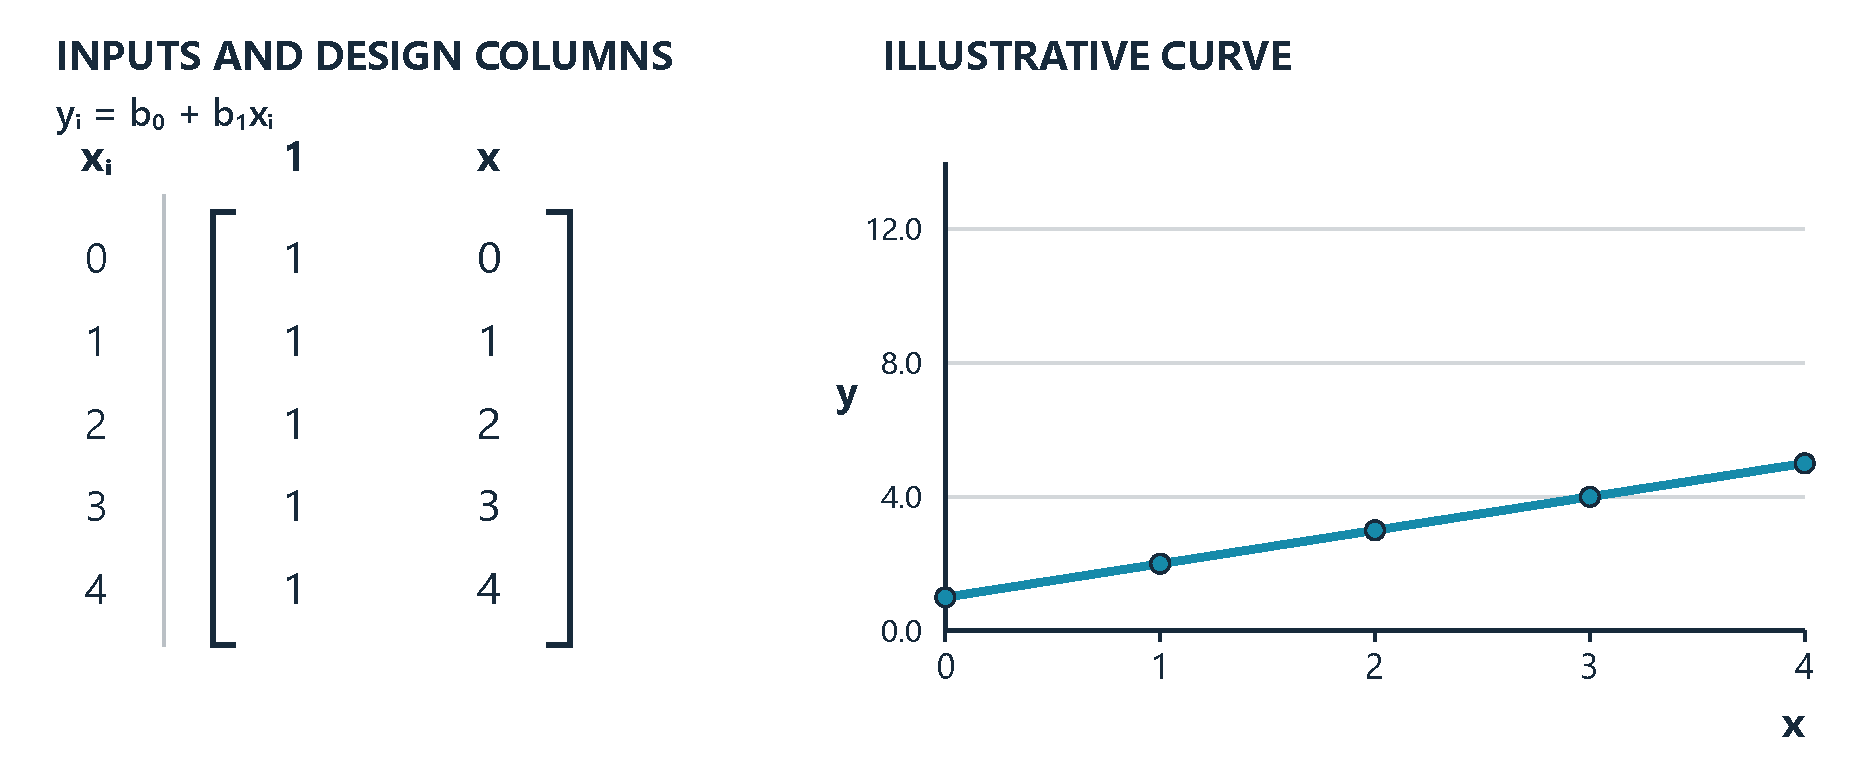
\includegraphics[width=\linewidth,height=.62\textheight,keepaspectratio]{asset-94393b4b1316b32bc82f82d35ebd3446cdea9ce3b9766903242f470416179861.pdf}\end{center}

\medskip

\textbf{Design matrix: intercept and squared term}


Keep the constant column and square every input in the second column. This column multiplies b\ensuremath{{}_2}. There is no b\ensuremath{{}_1} term. The parabola has its vertex at x = 0; only its right side is shown. The design and its curve appear together in \hyperref[material-a9d4aa1f590ca08fdbcd3c88af0c088204db86409807f830ed78fb7dd2600430]{Fig.~\ref*{material-a9d4aa1f590ca08fdbcd3c88af0c088204db86409807f830ed78fb7dd2600430}}.


\par\medskip
\Needspace{10cm}
\refstepcounter{figure}\label{material-a9d4aa1f590ca08fdbcd3c88af0c088204db86409807f830ed78fb7dd2600430}
\noindent\textbf{Fig.~\ref*{material-a9d4aa1f590ca08fdbcd3c88af0c088204db86409807f830ed78fb7dd2600430}.} Design matrix: intercept and squared term\par\nopagebreak
\begin{center}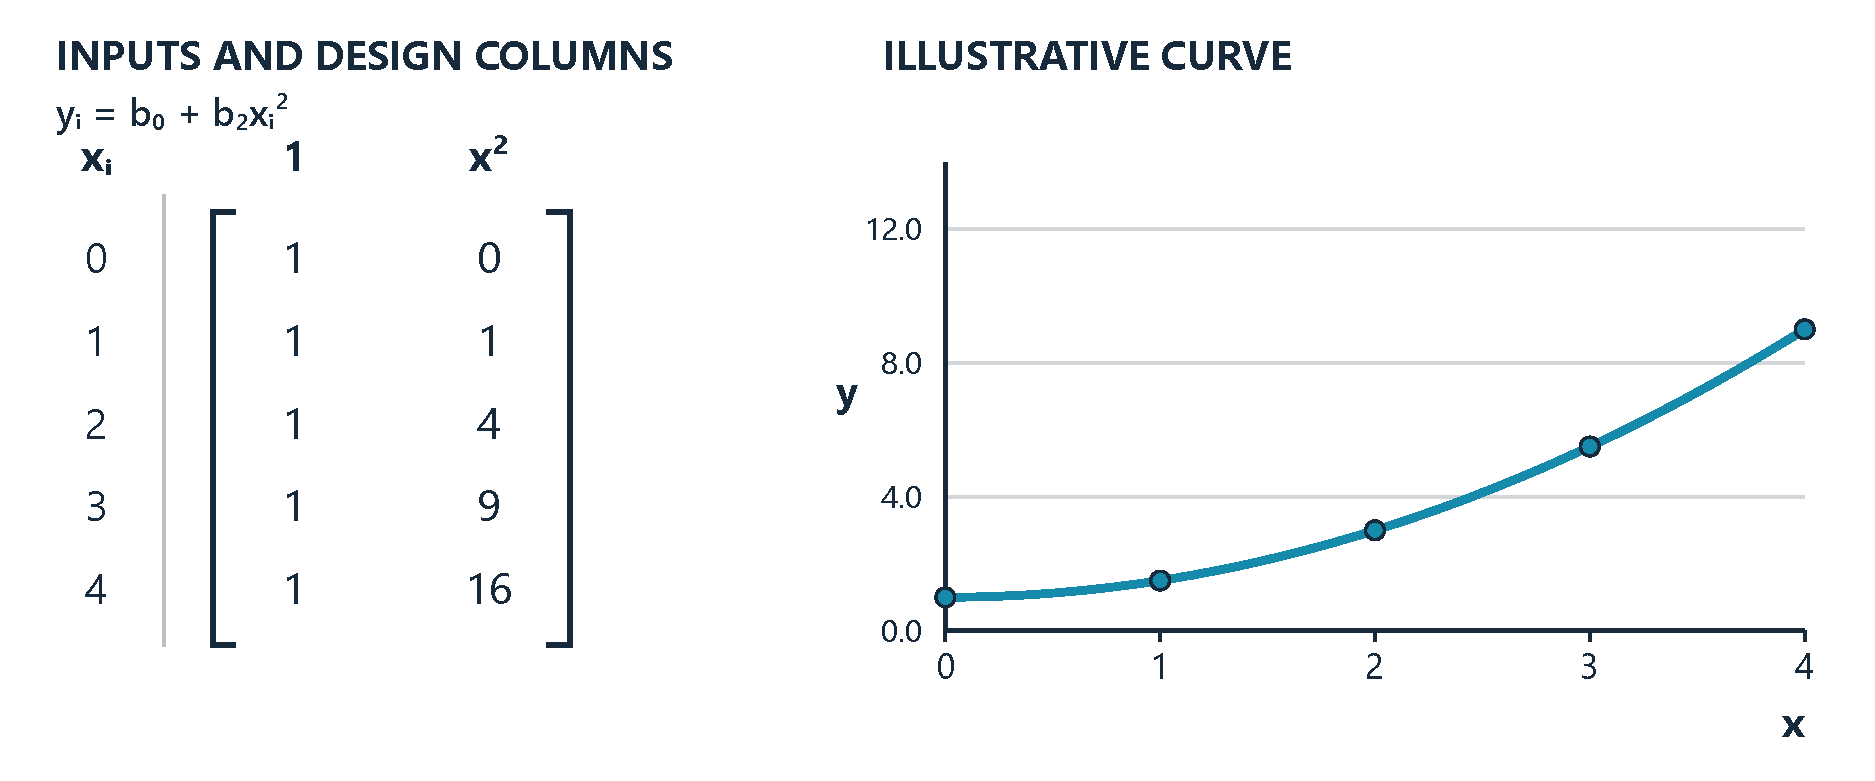
\includegraphics[width=\linewidth,height=.62\textheight,keepaspectratio]{asset-e3fb289f405785a9b9f9166c95fb12ad97731894bf34293b763360569568dabf.pdf}\end{center}

\medskip

\textbf{Design matrix: intercept, x and x\ensuremath{{}^2}}


Keep both transformed columns. The x term tilts the parabola and shifts its vertex. Higher powers x\ensuremath{{}^3} and x\ensuremath{{}^4} are further columns if the model calls for them. The design and its curve appear together in \hyperref[material-4b25e73fb8f9b89f74edcdf789d5eb31dc2604122951aa48cee44d8f26271173]{Fig.~\ref*{material-4b25e73fb8f9b89f74edcdf789d5eb31dc2604122951aa48cee44d8f26271173}}.


\par\medskip
\Needspace{10cm}
\refstepcounter{figure}\label{material-4b25e73fb8f9b89f74edcdf789d5eb31dc2604122951aa48cee44d8f26271173}
\noindent\textbf{Fig.~\ref*{material-4b25e73fb8f9b89f74edcdf789d5eb31dc2604122951aa48cee44d8f26271173}.} Design matrix: intercept, x and x\ensuremath{{}^2}\par\nopagebreak
\begin{center}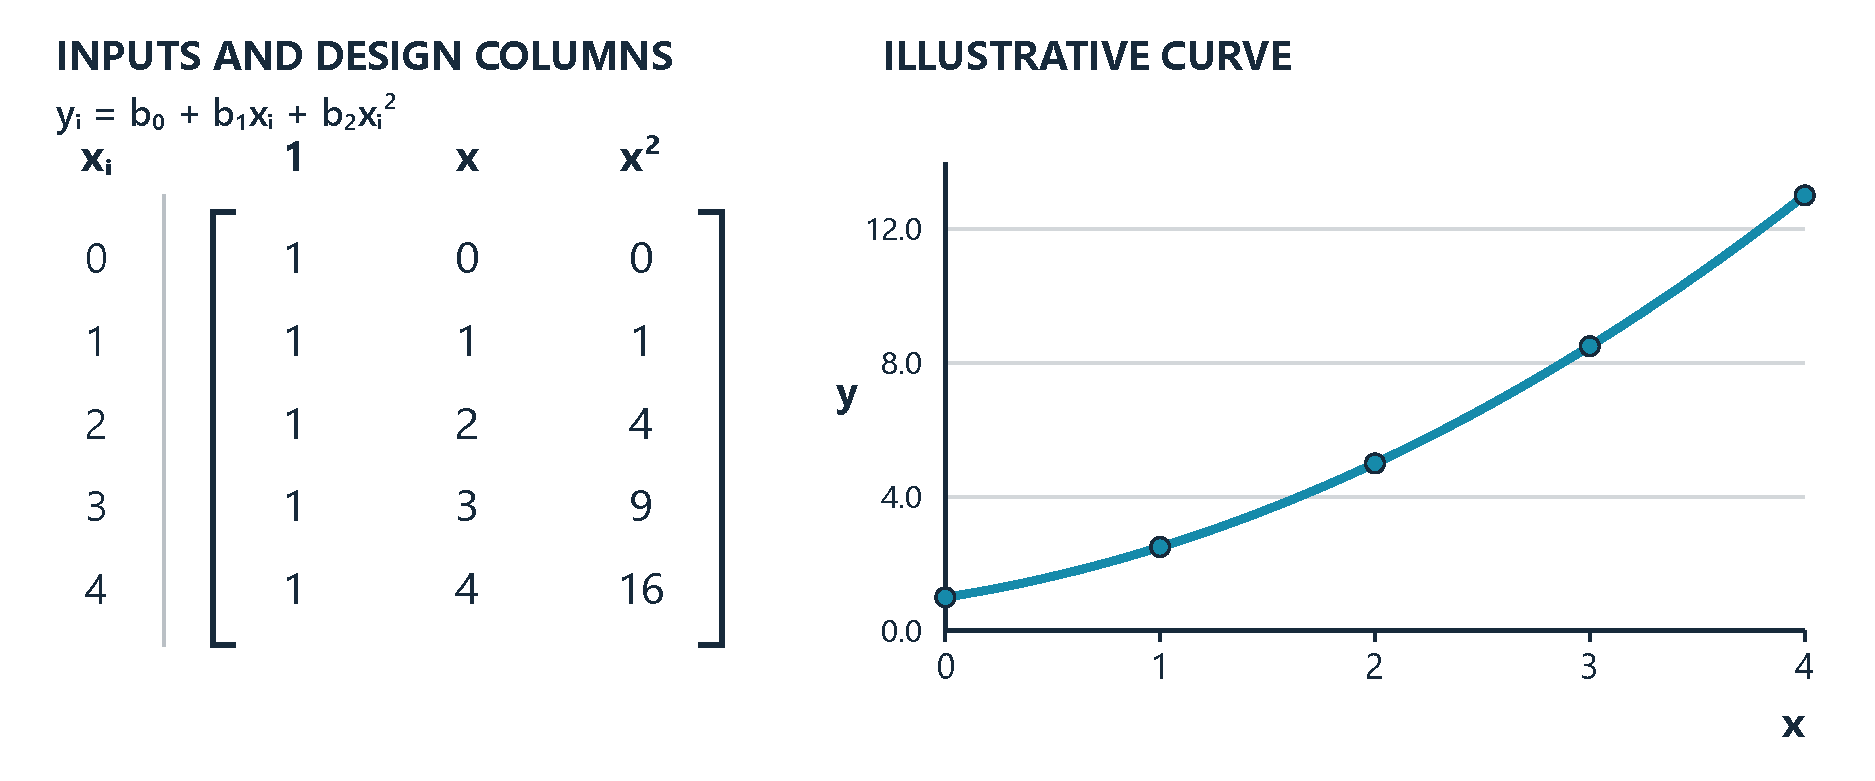
\includegraphics[width=\linewidth,height=.62\textheight,keepaspectratio]{asset-ece8745c84b355466ad617cd639695f589206a658f94a25cc641358b1d0b0d43.pdf}\end{center}

\medskip

\textbf{Design matrix: combine sinh and cosh}


Use dimensionless x. The sinh column changes sign across zero, while cosh has the same value at x and minus x. Their weights are independent. These are hyperbolic functions; a reciprocal term is a different way to obtain a hyperbola. The design and its curve appear together in \hyperref[material-9119ea9c3dde49ef3f00b5b72e876fc386c69a223511309f323ab2bb64e6b182]{Fig.~\ref*{material-9119ea9c3dde49ef3f00b5b72e876fc386c69a223511309f323ab2bb64e6b182}}.


\par\medskip
\Needspace{10cm}
\refstepcounter{figure}\label{material-9119ea9c3dde49ef3f00b5b72e876fc386c69a223511309f323ab2bb64e6b182}
\noindent\textbf{Fig.~\ref*{material-9119ea9c3dde49ef3f00b5b72e876fc386c69a223511309f323ab2bb64e6b182}.} Design matrix: combine sinh and cosh\par\nopagebreak
\begin{center}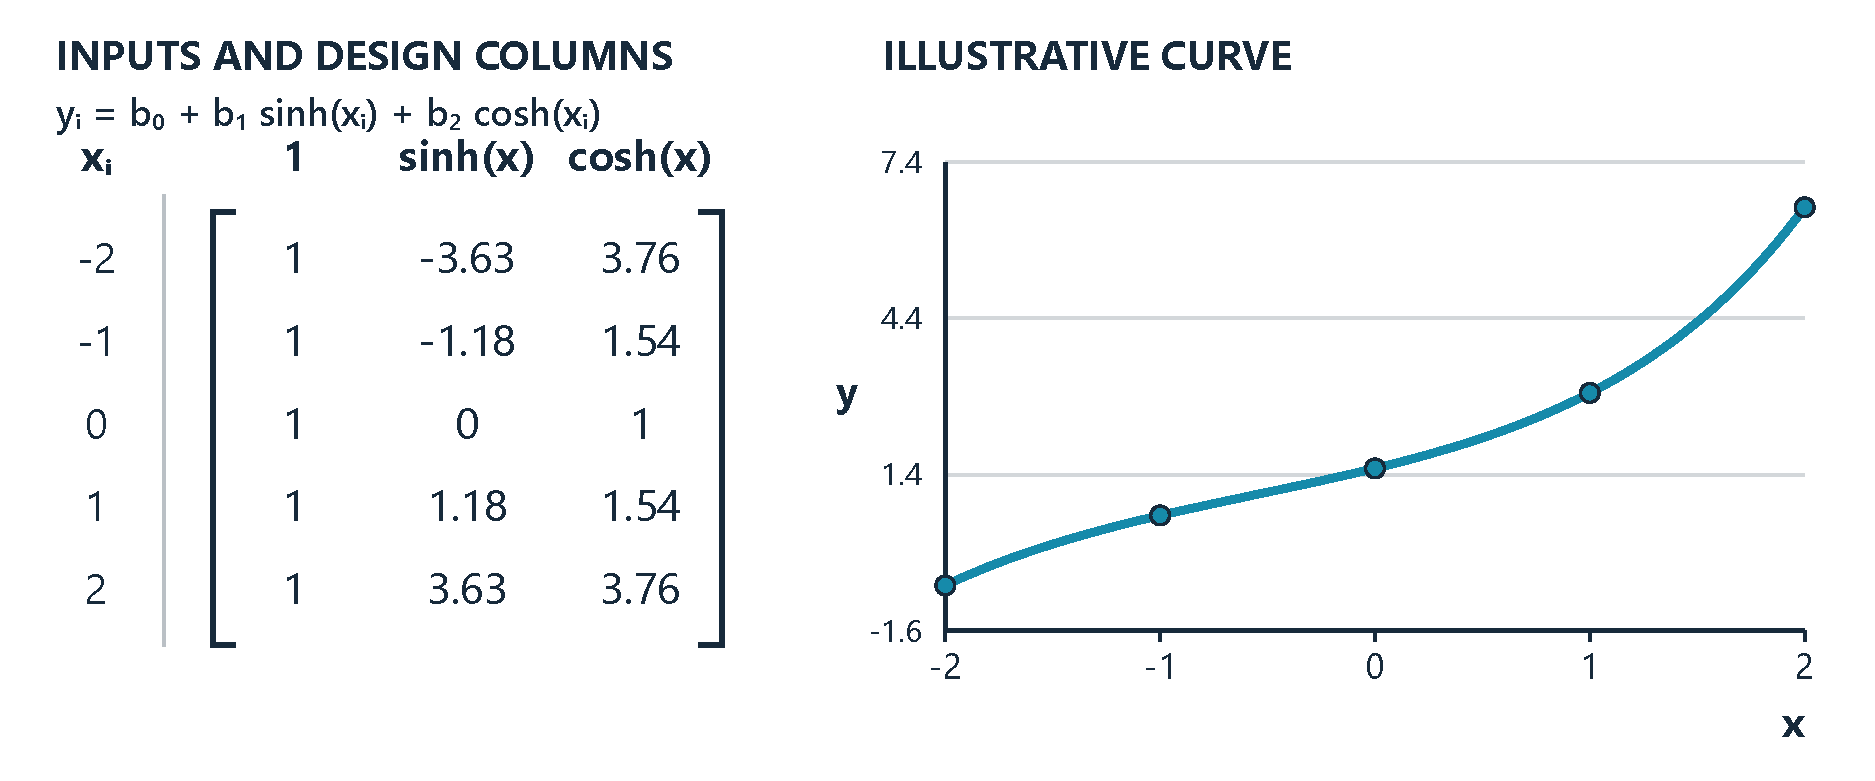
\includegraphics[width=\linewidth,height=.62\textheight,keepaspectratio]{asset-167550b772fe81af3353b23fcdf55150b94396f3dd4933edab6bf4988848fac1.pdf}\end{center}

\medskip

\textbf{Design matrix: exponential column}


Exponentiate each dimensionless input before fitting. The multiplier of exp(x) is a coefficient. If an unknown coefficient were placed inside the exponential, the model would no longer be linear in that coefficient. The design and its curve appear together in \hyperref[material-c1dce47edca968cdbfac5463ddb771a5753a08058c583508f643ff87121a59c3]{Fig.~\ref*{material-c1dce47edca968cdbfac5463ddb771a5753a08058c583508f643ff87121a59c3}}.


\par\medskip
\Needspace{10cm}
\refstepcounter{figure}\label{material-c1dce47edca968cdbfac5463ddb771a5753a08058c583508f643ff87121a59c3}
\noindent\textbf{Fig.~\ref*{material-c1dce47edca968cdbfac5463ddb771a5753a08058c583508f643ff87121a59c3}.} Design matrix: exponential column\par\nopagebreak
\begin{center}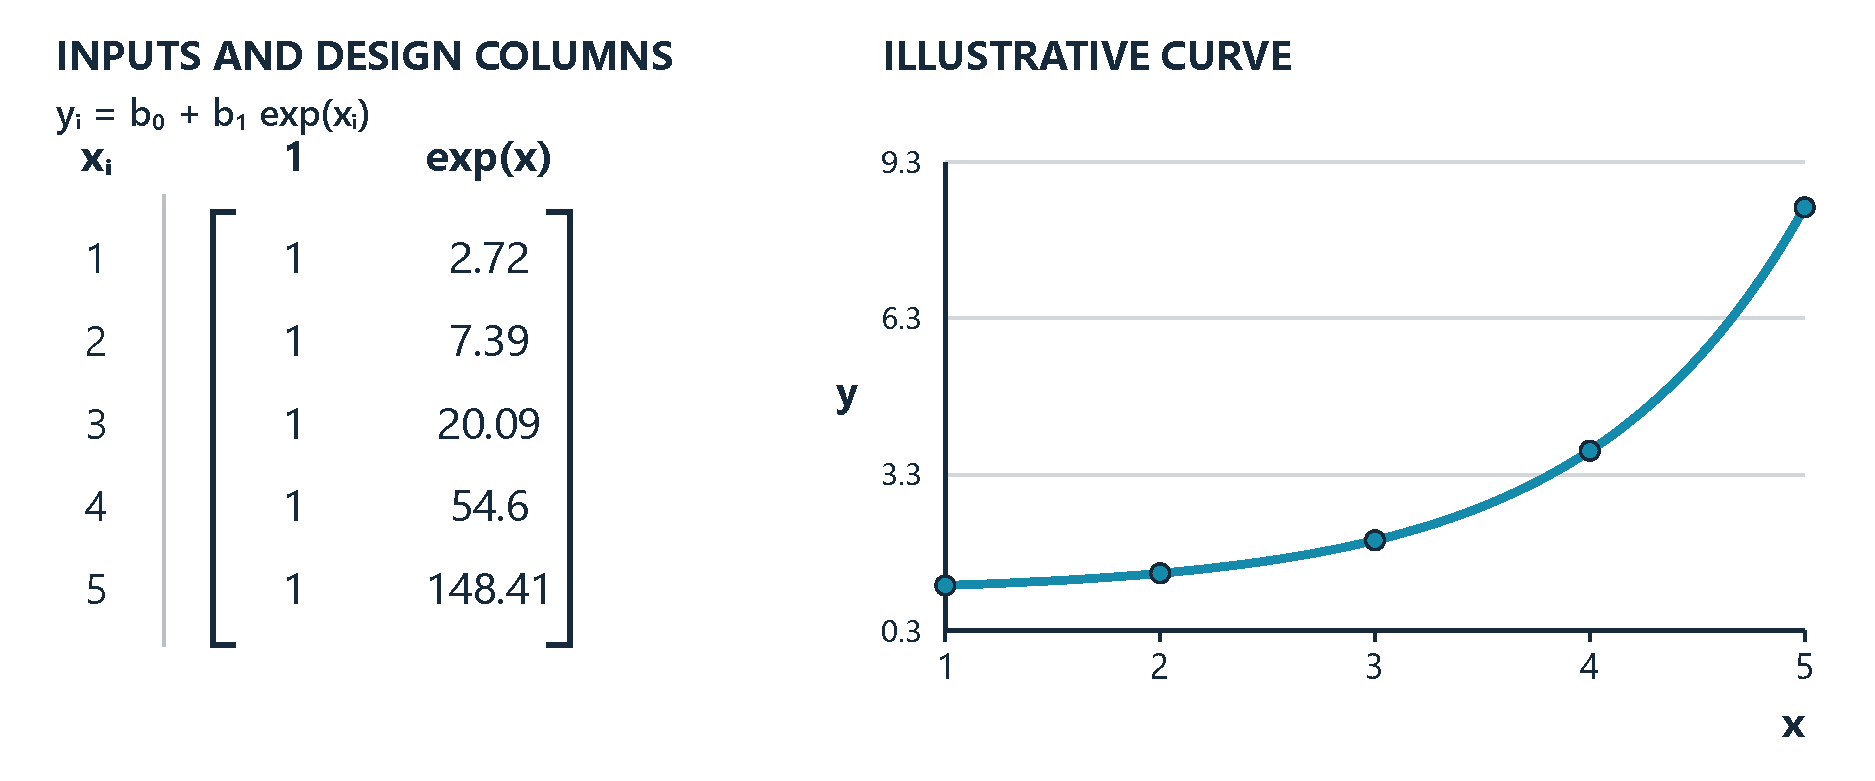
\includegraphics[width=\linewidth,height=.62\textheight,keepaspectratio]{asset-3c71bec8642e2dc676d333f7a93b9260a4d0b82962a296d34239e5887d8b57d9.pdf}\end{center}

\medskip

\textbf{Design matrix: logarithmic column}


Use positive, dimensionless inputs. The logarithm acts on x, while the response remains on its original scale. This differs from fitting a logarithm of the measured response. The design and its curve appear together in \hyperref[material-4fedde8beeb4d2e91aa56bc773cf4b09d47d0657ec95ef46cc842525c5718fad]{Fig.~\ref*{material-4fedde8beeb4d2e91aa56bc773cf4b09d47d0657ec95ef46cc842525c5718fad}}.


\par\medskip
\Needspace{10cm}
\refstepcounter{figure}\label{material-4fedde8beeb4d2e91aa56bc773cf4b09d47d0657ec95ef46cc842525c5718fad}
\noindent\textbf{Fig.~\ref*{material-4fedde8beeb4d2e91aa56bc773cf4b09d47d0657ec95ef46cc842525c5718fad}.} Design matrix: logarithmic column\par\nopagebreak
\begin{center}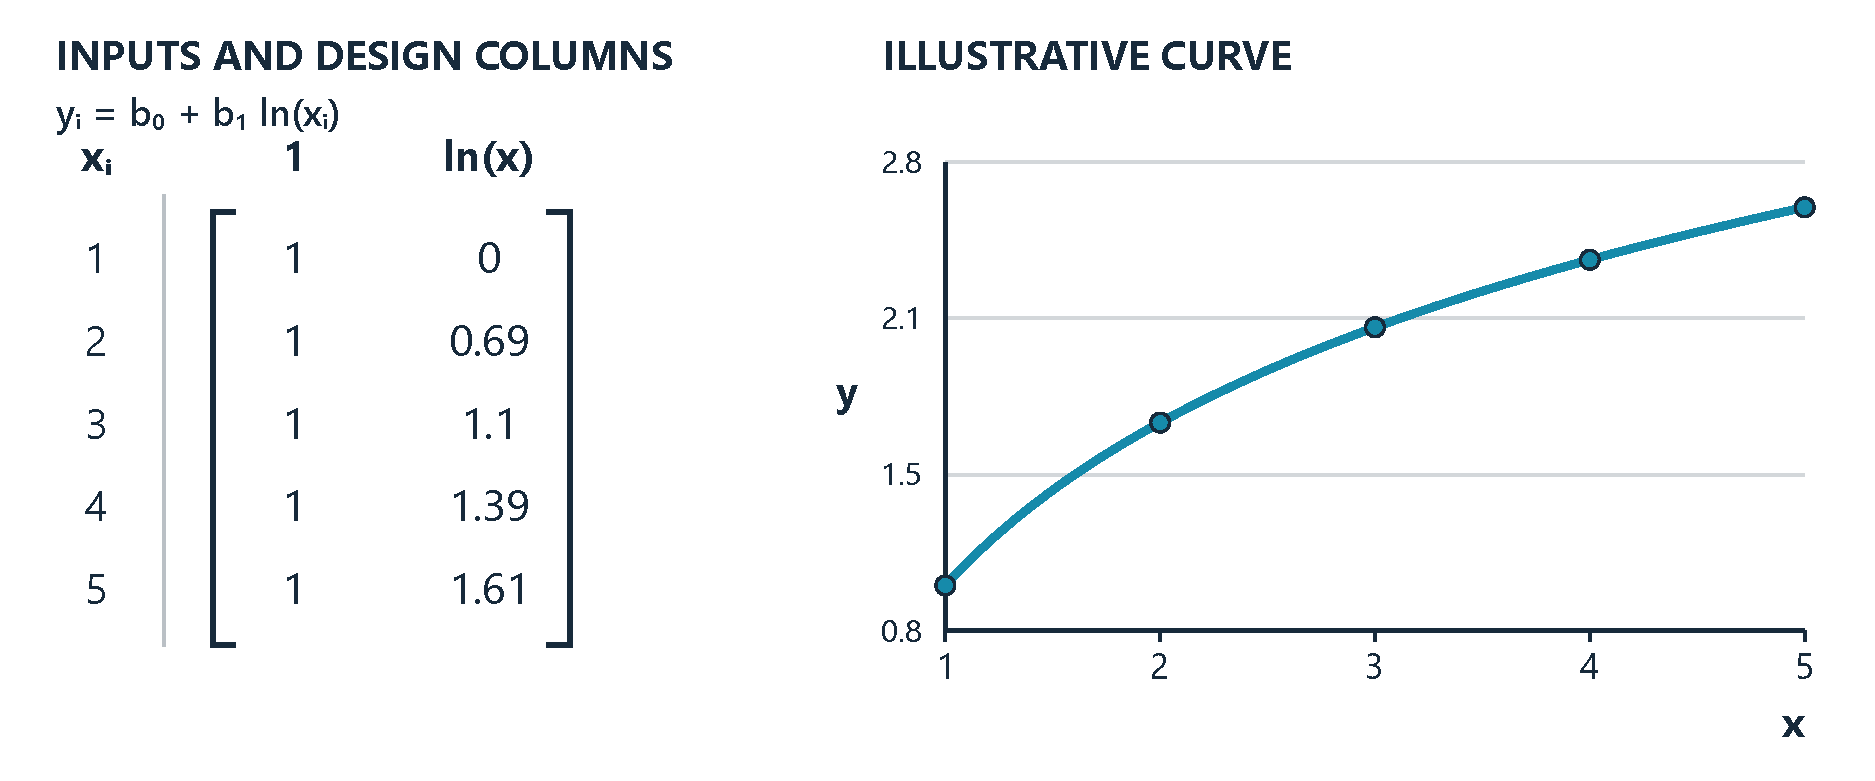
\includegraphics[width=\linewidth,height=.62\textheight,keepaspectratio]{asset-d53baf1792ca6628d55eefd31ac24a38034e872b477e53b69da9898aa7e6a374.pdf}\end{center}

\medskip

\textbf{Design matrix: reciprocal column}


Use nonzero x. Here the five inputs are positive and the curve tends toward the intercept. The reciprocal is undefined at zero, so never draw a continuous curve through zero. The design and its curve appear together in \hyperref[material-5414a7b4cf494b74f57d4a1f4bb51a0ea75f759a7640fb2a36edf0c7304a1ec5]{Fig.~\ref*{material-5414a7b4cf494b74f57d4a1f4bb51a0ea75f759a7640fb2a36edf0c7304a1ec5}}.


\par\medskip
\Needspace{10cm}
\refstepcounter{figure}\label{material-5414a7b4cf494b74f57d4a1f4bb51a0ea75f759a7640fb2a36edf0c7304a1ec5}
\noindent\textbf{Fig.~\ref*{material-5414a7b4cf494b74f57d4a1f4bb51a0ea75f759a7640fb2a36edf0c7304a1ec5}.} Design matrix: reciprocal column\par\nopagebreak
\begin{center}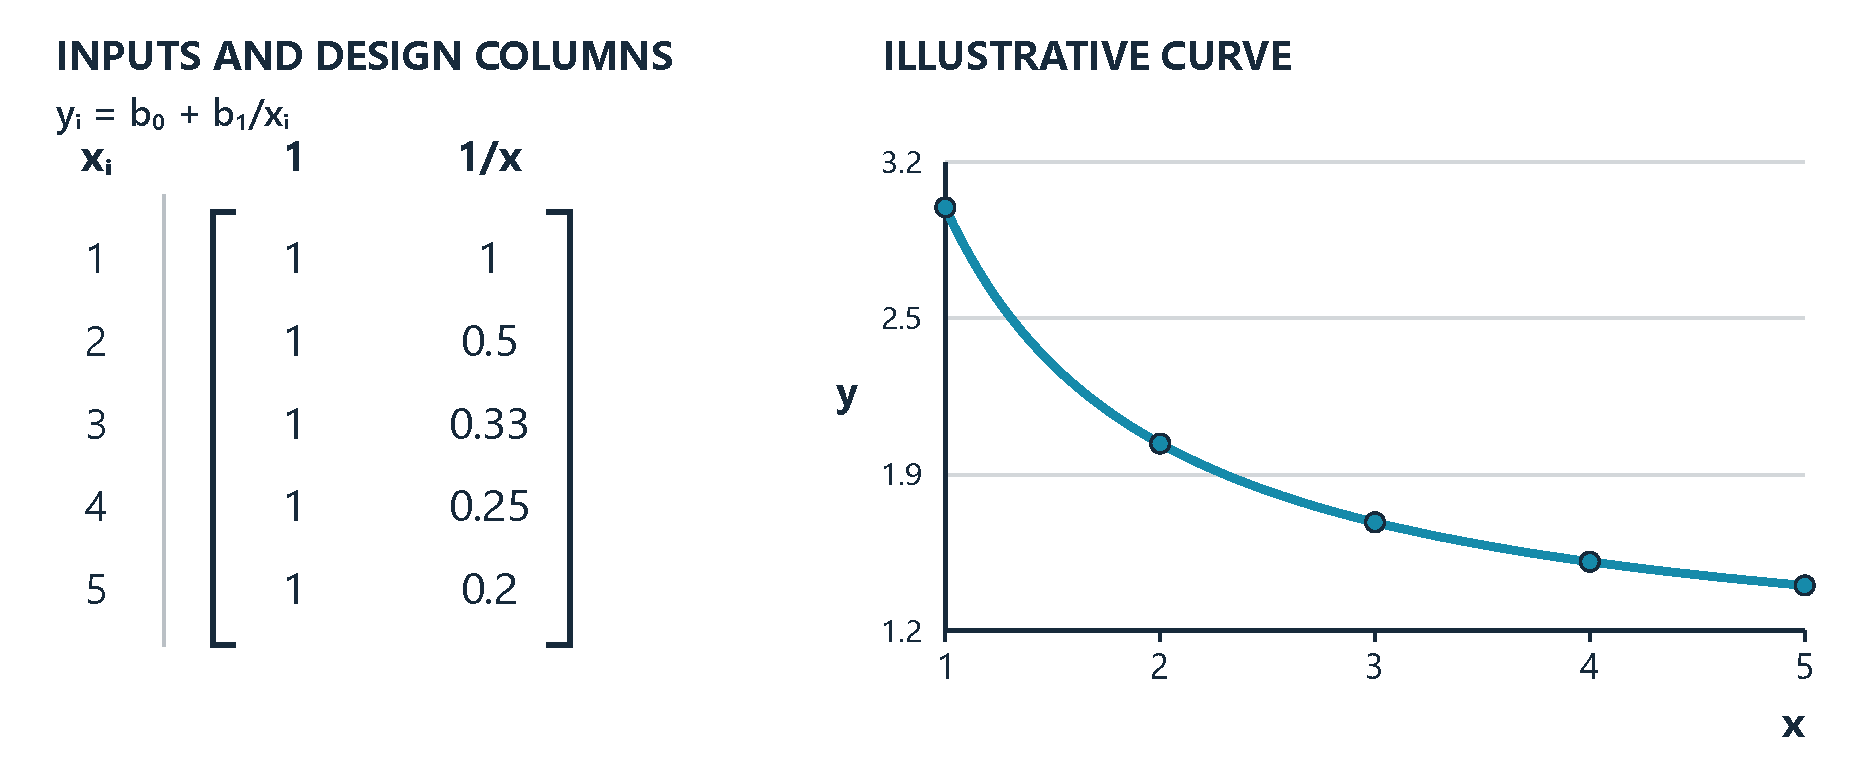
\includegraphics[width=\linewidth,height=.62\textheight,keepaspectratio]{asset-5d150f543965c8f576b9b95fb564004529dc23a38c84ee510774030b8416dbe6.pdf}\end{center}

\medskip

\textbf{Design matrix: square-root column}


For real-valued square roots, x must be nonnegative. This case uses the same five positive inputs as the exponential, logarithm and reciprocal examples. The transform is fixed before fitting. The design and its curve appear together in \hyperref[material-ebf9bcba0b232275f94d64391bdd71208e6b3f8bdf154ffa7083593ee3f44b6a]{Fig.~\ref*{material-ebf9bcba0b232275f94d64391bdd71208e6b3f8bdf154ffa7083593ee3f44b6a}}.


\par\medskip
\Needspace{10cm}
\refstepcounter{figure}\label{material-ebf9bcba0b232275f94d64391bdd71208e6b3f8bdf154ffa7083593ee3f44b6a}
\noindent\textbf{Fig.~\ref*{material-ebf9bcba0b232275f94d64391bdd71208e6b3f8bdf154ffa7083593ee3f44b6a}.} Design matrix: square-root column\par\nopagebreak
\begin{center}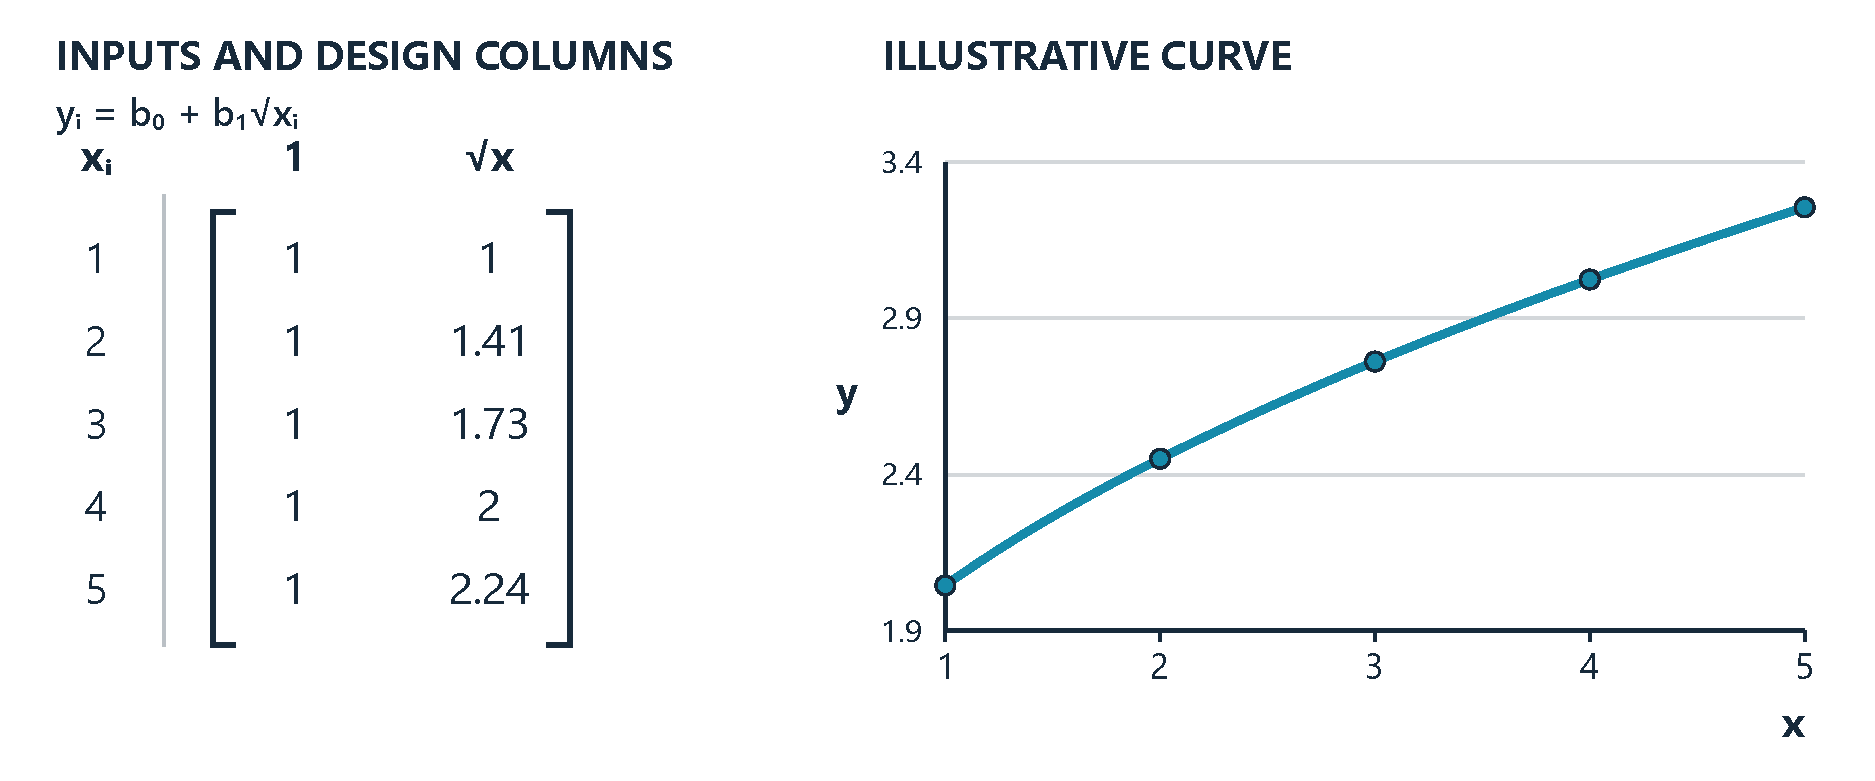
\includegraphics[width=\linewidth,height=.62\textheight,keepaspectratio]{asset-05fe86c84936be18a7c0637f29f9da9f4499b8641dd558b2499df684a9c1bf7d.pdf}\end{center}

\medskip

\textbf{Design matrix: mix several functions}


The first five rows and a curve for chosen weights appear in \hyperref[material-fefe7287b10e61f9198b6157f41ac5181dfd68970ed9c5a7a9a298baf99f4657]{Fig.~\ref*{material-fefe7287b10e61f9198b6157f41ac5181dfd68970ed9c5a7a9a298baf99f4657}}. The coefficient vector is (4, \ensuremath{-}0.15, 1.5, \ensuremath{-}1.2, 1.1, \ensuremath{-}2, 0.9) in the same order as the columns. Each additional fixed function comes with its own weight. The five displayed rows alone cannot identify all seven weights.


\par\medskip
\Needspace{10cm}
\refstepcounter{figure}\label{material-fefe7287b10e61f9198b6157f41ac5181dfd68970ed9c5a7a9a298baf99f4657}
\noindent\textbf{Fig.~\ref*{material-fefe7287b10e61f9198b6157f41ac5181dfd68970ed9c5a7a9a298baf99f4657}.} Design matrix: mix several functions\par\nopagebreak
\begin{center}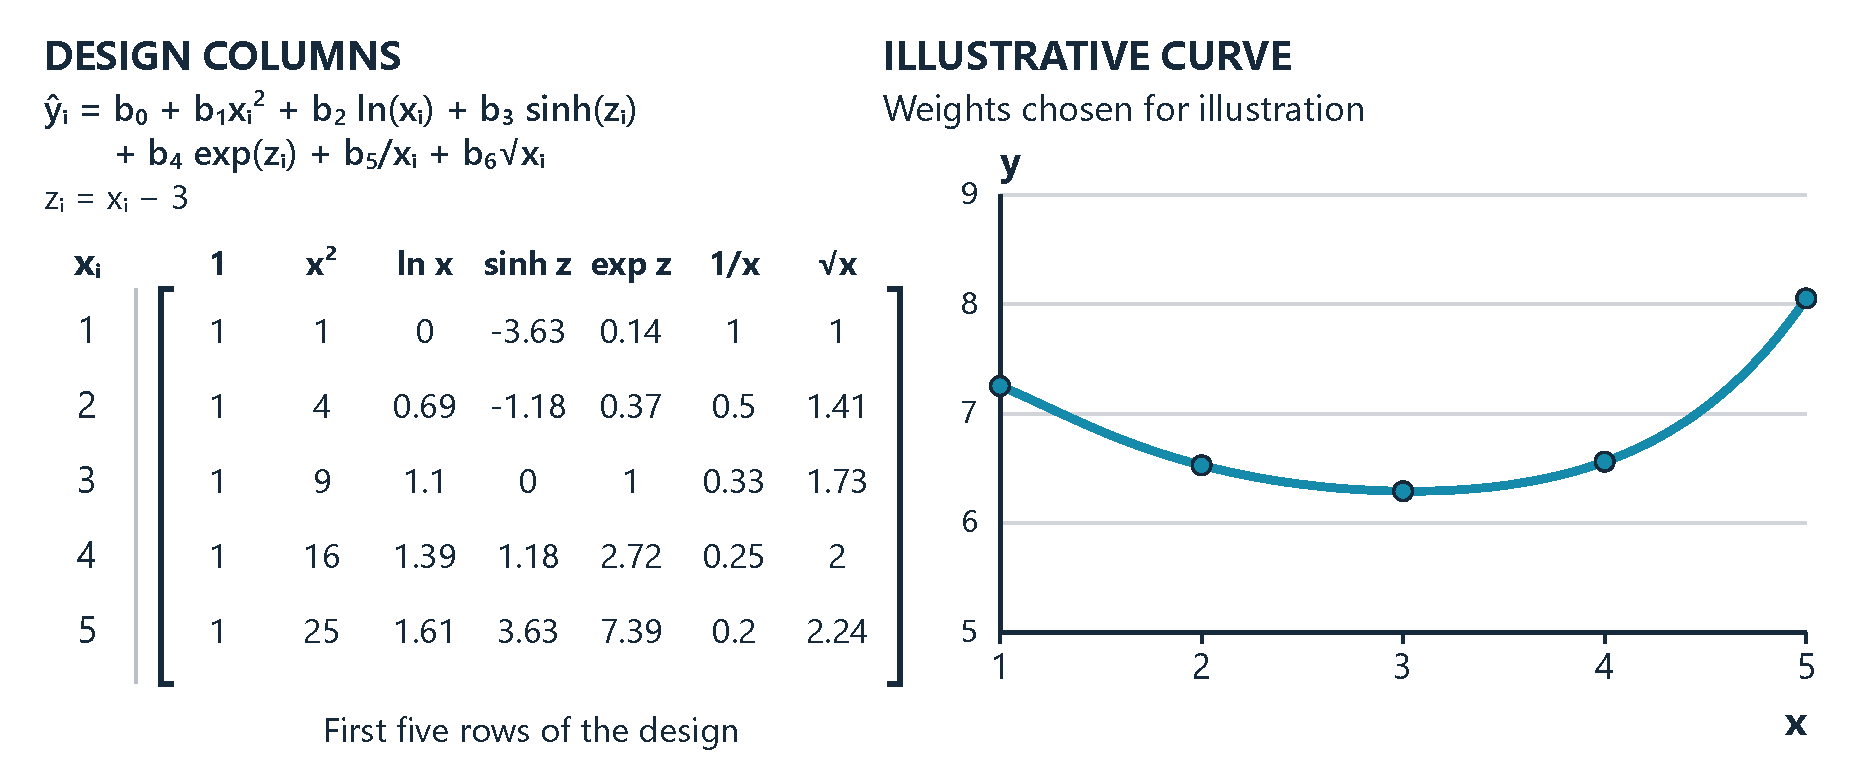
\includegraphics[width=\linewidth,height=.62\textheight,keepaspectratio]{asset-79dec64c45ee4c4655653cd30ac90741350b9bb84095615aaee08cc3d2dc3160.pdf}\end{center}

\medskip

\textbf{How many columns can we fit?}


Read \hyperref[material-62101aba735456c89aeccbe71e8390b41ca417458d968c176481a000442f29f7]{Eq.~\ref*{material-62101aba735456c89aeccbe71e8390b41ca417458d968c176481a000442f29f7}} with \(p\) counting all estimated coefficients, including the intercept. A unique ordinary least-squares solution requires independent columns, which implies \(p\leq n\). With \(p=n\) and full rank, the fit interpolates the data and leaves zero residual degrees of freedom. If we want at least one residual degree of freedom, use \(p\leq n-1\). This count is necessary; we still need to check column independence.


\par\medskip
\noindent\begin{minipage}{\linewidth}
\refstepcounter{equation}\label{material-62101aba735456c89aeccbe71e8390b41ca417458d968c176481a000442f29f7}
\noindent\textbf{Eq.~\ref*{material-62101aba735456c89aeccbe71e8390b41ca417458d968c176481a000442f29f7}.} How many columns can we fit?\par\nopagebreak
\begin{center}\begin{adjustbox}{max width=\linewidth}$\displaystyle \begin{aligned}\mathrm{df}_{\mathrm{res}}&=n-p\qquad\text{for independent columns}\\[.5em]n=5,\ p=4&:\quad 5-4=1 \quad\text{residual degree left}\\[.35em]n=5,\ p=5&:\quad 5-5=0 \quad\text{exact interpolation}\\[.35em]n=5,\ p=7&:\quad \text{no unique coefficient fit}\end{aligned}$\end{adjustbox}\end{center}

\par\noindent\textbf{Symbols}

\par\noindent\textbf{\(=,-,\leq\)} Equality, subtraction, and less than or equal to.

\par\noindent\textbf{\(\mathrm{df}_{\mathrm{res}}\)} Residual degrees of freedom: the number of observation directions left after fitting independent columns.

\par\noindent\textbf{\(n\)} Number of observation rows.

\par\noindent\textbf{\(p\)} Number of fitted coefficient columns, including the intercept if present.

\end{minipage}\par
\medskip

\textbf{Design matrix: eight rows for seven coefficients}


In \hyperref[material-1a4c17c623c5f7cc104b7885ec667eb55e5be63f171744c4e46eb5366ee024e2]{Fig.~\ref*{material-1a4c17c623c5f7cc104b7885ec667eb55e5be63f171744c4e46eb5366ee024e2}}, add three input rows at 1.5, 2.5 and 3.5 to the five-row design. At full precision, the seven columns are independent. Given eight observed responses, the coefficient fit is unique and the residual degrees of freedom are \(8-7=1\). The curve uses the same chosen weights as the previous illustration.


\par\medskip
\Needspace{10cm}
\refstepcounter{figure}\label{material-1a4c17c623c5f7cc104b7885ec667eb55e5be63f171744c4e46eb5366ee024e2}
\noindent\textbf{Fig.~\ref*{material-1a4c17c623c5f7cc104b7885ec667eb55e5be63f171744c4e46eb5366ee024e2}.} Design matrix: eight rows for seven coefficients\par\nopagebreak
\begin{center}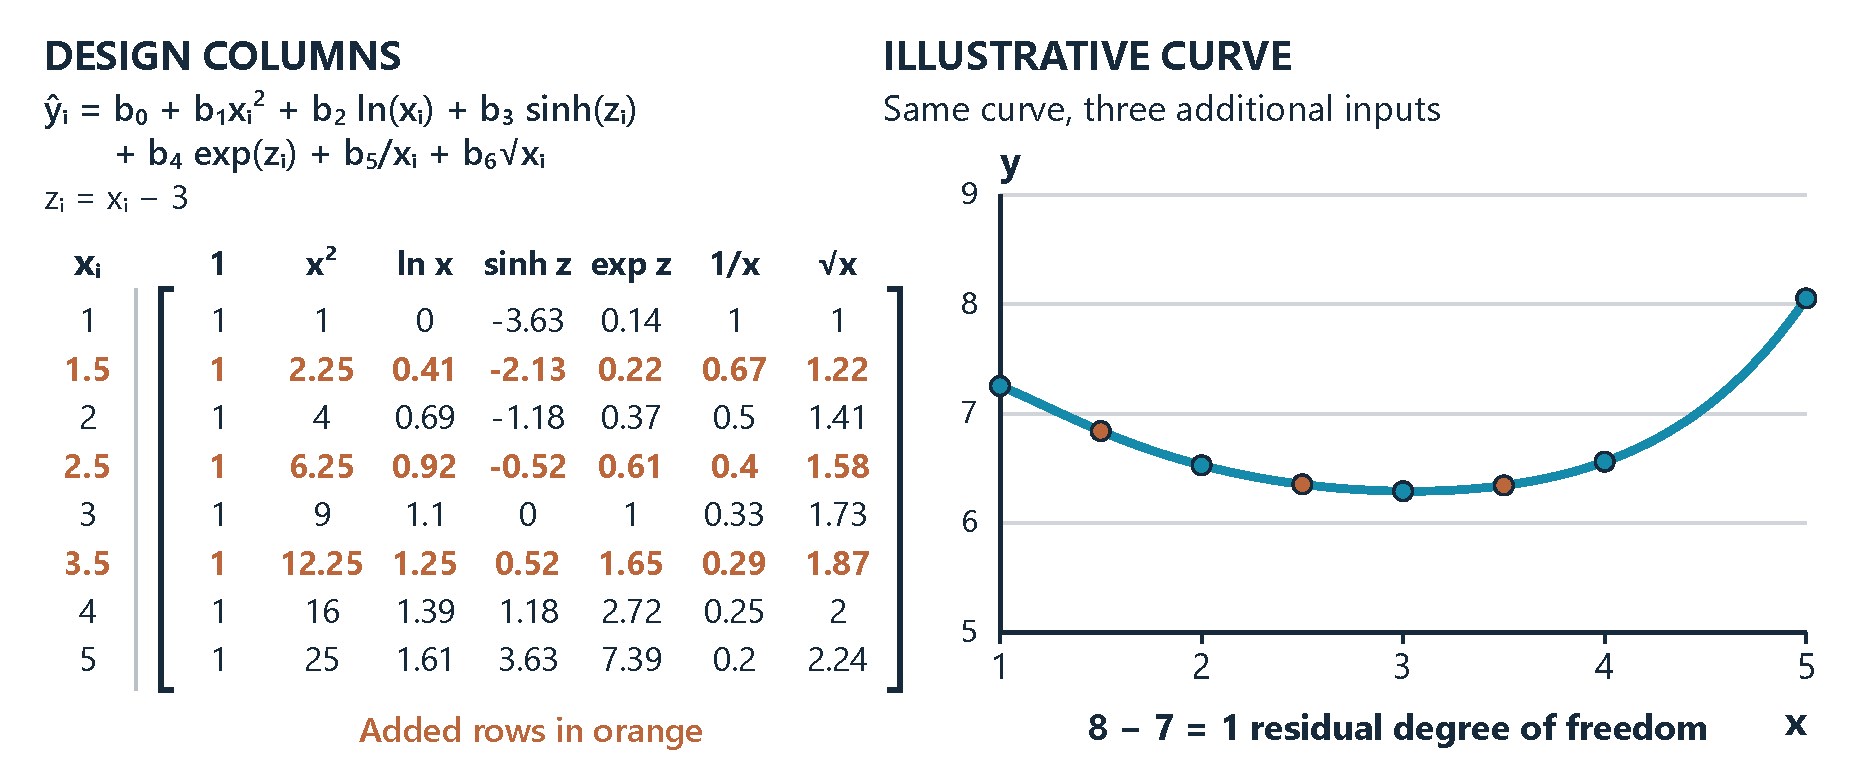
\includegraphics[width=\linewidth,height=.62\textheight,keepaspectratio]{asset-2f7a00a8f14dafd2e8d8a4f47fa4c780c85faffc32824c5618fca0f9fdf5473a.pdf}\end{center}

\medskip

\textbf{When is a model linear in its coefficients?}


The comparisons in \hyperref[material-901b1a37e86d272d3baef76094b627c97569018b7036d13a8f0d6b85461fe123]{Eq.~\ref*{material-901b1a37e86d272d3baef76094b627c97569018b7036d13a8f0d6b85461fe123}} use the same design-matrix rule: a term of the form \(b_j f_j(x)\) contributes the fixed column \(f_j(x)\). In \(\sinh(xb_4)\) and \(\exp(xb_2)\), the unknown changes the column itself, so fitting the original coefficient requires nonlinear regression. In \(\exp(x+b_2)\), factor out \(\exp(b_2)\) and fit \(u\) as the new linear coefficient multiplying the known column \(\exp(x)\). A real \(b_2=\ln(u)\) can only be recovered for \(u>0\). If an unconstrained fit gives \(u\leq 0\), it does not correspond to the original model.


\par\medskip
\noindent\begin{minipage}{\linewidth}
\refstepcounter{equation}\label{material-901b1a37e86d272d3baef76094b627c97569018b7036d13a8f0d6b85461fe123}
\noindent\textbf{Eq.~\ref*{material-901b1a37e86d272d3baef76094b627c97569018b7036d13a8f0d6b85461fe123}.} When is a model linear in its coefficients?\par\nopagebreak
\begin{center}\begin{adjustbox}{max width=\linewidth}$\displaystyle \begin{aligned}\text{Fixed column:}&\quad b_4\sinh(x),\quad b_2\exp(x)\\[.55em]\text{Column depends on coefficient:}&\quad \sinh(xb_4),\quad \exp(xb_2)\\[.55em]\text{Reparameterise:}&\quad \exp(x+b_2)=\exp(b_2)\exp(x)\\[.25em]&\quad =\underbrace{u}_{\text{linear coefficient}}\,\exp(x),\qquad u=\exp(b_2)>0\end{aligned}$\end{adjustbox}\end{center}

\par\noindent\textbf{Symbols}

\par\noindent\textbf{\(+,=,>,0\)} Addition, equality, and greater than zero. Juxtaposition indicates multiplication.

\par\noindent\textbf{\(\sinh,\exp\)} Hyperbolic sine and exponential functions.

\par\noindent\textbf{\(b_2,b_4\)} Unknown model coefficients. The subscripts distinguish the examples.

\par\noindent\textbf{\(u\)} New coefficient equal to exp(b\ensuremath{{}_2}). It must be positive to correspond to a real b\ensuremath{{}_2}.

\par\noindent\textbf{\(x\)} Known dimensionless input. Its transformed values form a design column.

\end{minipage}\par
\medskip

\textbf{Five inputs, three design columns}


The matrix and model curve appear together in \hyperref[material-8354997b9d405354138c428c7bc01256194f905f6161517491d248dad2c5aa73]{Fig.~\ref*{material-8354997b9d405354138c428c7bc01256194f905f6161517491d248dad2c5aa73}}. Use the five input values 1, 4, 9, 16 and 25. The columns are the constant one, x itself and the square root of x. The plotted curve is Xb at those inputs and the same model evaluated between them, using chosen coefficients.


\par\medskip
\Needspace{10cm}
\refstepcounter{figure}\label{material-8354997b9d405354138c428c7bc01256194f905f6161517491d248dad2c5aa73}
\noindent\textbf{Fig.~\ref*{material-8354997b9d405354138c428c7bc01256194f905f6161517491d248dad2c5aa73}.} Five inputs, three design columns\par\nopagebreak
\begin{center}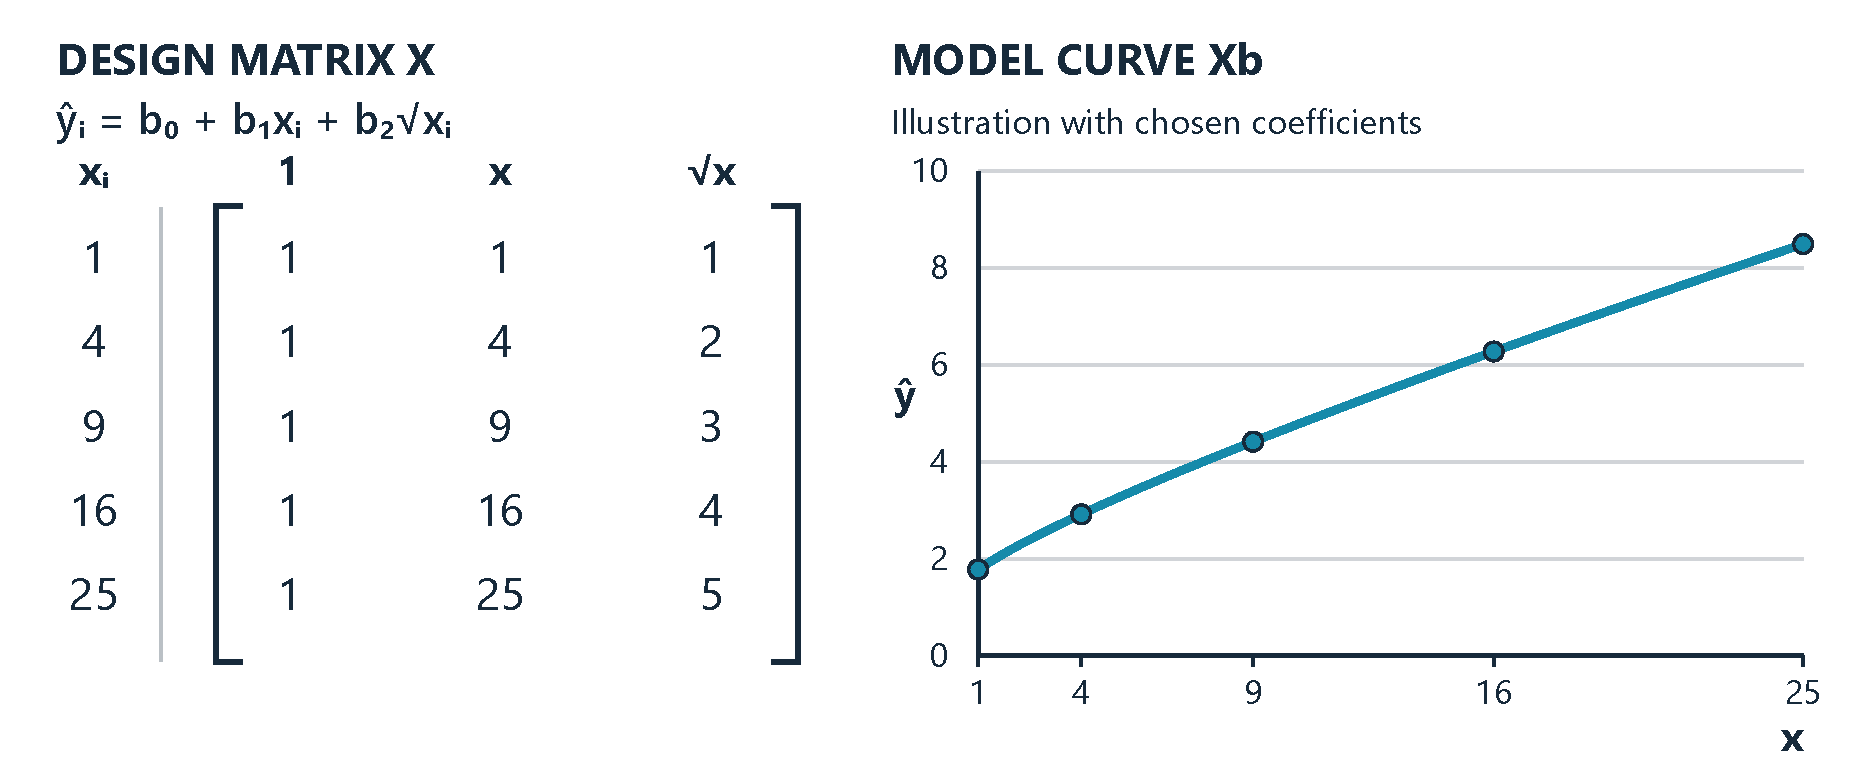
\includegraphics[width=\linewidth,height=.62\textheight,keepaspectratio]{asset-0b8a5ebca75e11387ad05c49c133396efc9bb0fe838a12cc984f4a1c31e46381.pdf}\end{center}

\medskip

\textbf{From one squared length to X\ensuremath{{}^{\mathsf T}}X}


Apply the column-product rule from \hyperref[material-6733cde141c87d89df5364052b6cc49fcfc9897b6f6bcb92b71c89a40b0fd3a3]{Eq.~\ref*{material-6733cde141c87d89df5364052b6cc49fcfc9897b6f6bcb92b71c89a40b0fd3a3}} to each pair in \hyperref[material-6887f050e33647d8433b3a2f0bdc4adf9455056696ea22c049054e843cadfa9d]{Eq.~\ref*{material-6887f050e33647d8433b3a2f0bdc4adf9455056696ea22c049054e843cadfa9d}}. Recall that e transpose e is one dot product of a column with itself. X transpose X applies that rule to every pair of columns. A diagonal entry sums squares of one column. An off-diagonal entry sums products of two different columns in matching rows.


\par\medskip
\noindent\begin{minipage}{\linewidth}
\refstepcounter{equation}\label{material-6887f050e33647d8433b3a2f0bdc4adf9455056696ea22c049054e843cadfa9d}
\noindent\textbf{Eq.~\ref*{material-6887f050e33647d8433b3a2f0bdc4adf9455056696ea22c049054e843cadfa9d}.} From one squared length to X\ensuremath{{}^{\mathsf T}}X\par\nopagebreak
\begin{center}\begin{adjustbox}{max width=\linewidth}$\displaystyle \begin{aligned}e^{\mathsf T}e&=\sum_{i=1}^n e_i^2 &&\text{one column, one squared length}\\[.65em](X^{\mathsf T}X)_{jk}&=c_j^{\mathsf T}c_k=\sum_{i=1}^n c_{ij}c_{ik} &&\text{one entry for every column pair}\end{aligned}$\end{adjustbox}\end{center}

\par\noindent\textbf{Symbols}

\par\noindent\textbf{\(+,=,\cdot\)} Addition, equality and multiplication. Juxtaposition multiplies, and a power of 2 squares the term.

\par\noindent\textbf{\(X\)} Design matrix whose columns are 1, x and the square root of x.

\par\noindent\textbf{\(\sum_{i=1}^{n}\)} Add across all n observation rows.

\par\noindent\textbf{\(c_j,c_k,j,k\)} Design columns j and k. Here column 1 contains ones, column 2 contains x and column 3 contains square roots.

\par\noindent\textbf{\(e\)} Column of all residuals, one per observation.

\par\noindent\textbf{\(e_i,c_{ij},i,n\)} Residual at row i and entry at row i of design column j. The row index runs from 1 to the sample count n.

\par\noindent\textbf{\({}^{\mathsf T}\)} Transpose, interchanging rows and columns.

\end{minipage}\par
\medskip

\textbf{Calculate X\ensuremath{{}^{\mathsf T}}X for the five inputs}


Use the design and curve in \hyperref[material-8354997b9d405354138c428c7bc01256194f905f6161517491d248dad2c5aa73]{Fig.~\ref*{material-8354997b9d405354138c428c7bc01256194f905f6161517491d248dad2c5aa73}} as context for the matrix calculation in \hyperref[material-b92dcc37b0020d5f2ab4b2cad626634e38c10e509c2e32320634e4f2ad0a2e75]{Eq.~\ref*{material-b92dcc37b0020d5f2ab4b2cad626634e38c10e509c2e32320634e4f2ad0a2e75}}. Read the second column as x and the third as square roots. Multiply matching entries and sum. To get the second diagonal entry, square every x and add. To get entry row two, column three, multiply x by its square root in each row and add. Its mirror entry has the same value. Repeat with the column of ones and the third column to complete the matrix.


\par\medskip
\noindent\begin{minipage}{\linewidth}
\refstepcounter{equation}\label{material-b92dcc37b0020d5f2ab4b2cad626634e38c10e509c2e32320634e4f2ad0a2e75}
\noindent\textbf{Eq.~\ref*{material-b92dcc37b0020d5f2ab4b2cad626634e38c10e509c2e32320634e4f2ad0a2e75}.} Calculate X\ensuremath{{}^{\mathsf T}}X for the five inputs\par\nopagebreak
\begin{center}\begin{adjustbox}{max width=\linewidth}$\displaystyle \begin{aligned}c_2^{\mathsf T}c_2&=1^2+4^2+9^2+16^2+25^2=979\\[.35em]c_2^{\mathsf T}c_3&=1\cdot1+4\cdot2+9\cdot3+16\cdot4+25\cdot5=225\\[.5em]X^{\mathsf T}X&=\begin{bmatrix}5&55&15\\55&979&225\\15&225&55\end{bmatrix}\end{aligned}$\end{adjustbox}\end{center}

\par\noindent\textbf{Symbols}

\par\noindent\textbf{\(+,=,\cdot\)} Addition, equality and multiplication. Juxtaposition multiplies, and a power of 2 squares the term.

\par\noindent\textbf{\(X\)} Design matrix whose columns are 1, x and the square root of x.

\par\noindent\textbf{\(c_j,c_k,j,k\)} Design columns j and k. Here column 1 contains ones, column 2 contains x and column 3 contains square roots.

\par\noindent\textbf{\({}^{\mathsf T}\)} Transpose, interchanging rows and columns.

\end{minipage}\par
\medskip

\textbf{Calculate X\ensuremath{{}^{\mathsf T}}y from the measured responses}


In \hyperref[material-a9e30ba9602493bcc159c3cd3ed0a9fa10daafdbf634aa94924a750817bba5c4]{Eq.~\ref*{material-a9e30ba9602493bcc159c3cd3ed0a9fa10daafdbf634aa94924a750817bba5c4}}, use the same design as in \hyperref[material-8354997b9d405354138c428c7bc01256194f905f6161517491d248dad2c5aa73]{Fig.~\ref*{material-8354997b9d405354138c428c7bc01256194f905f6161517491d248dad2c5aa73}} and add a column of measured responses. Keep the same five input rows and align the example measurements 2, 3, 5, 6 and 9 with them in order. Multiply each design column entry by the matching measured response and add the five products. The constant column gives the response sum, the x column gives 380, and the square-root column gives 92. This is the right-hand side of the normal equation.


\par\medskip
\noindent\begin{minipage}{\linewidth}
\refstepcounter{equation}\label{material-a9e30ba9602493bcc159c3cd3ed0a9fa10daafdbf634aa94924a750817bba5c4}
\noindent\textbf{Eq.~\ref*{material-a9e30ba9602493bcc159c3cd3ed0a9fa10daafdbf634aa94924a750817bba5c4}.} Calculate X\ensuremath{{}^{\mathsf T}}y from the measured responses\par\nopagebreak
\begin{center}\begin{adjustbox}{max width=\linewidth}$\displaystyle \begin{aligned}X^{\mathsf T}y&=\begin{bmatrix}1&1&1&1&1\\1&4&9&16&25\\1&2&3&4&5\end{bmatrix}\begin{bmatrix}2\\3\\5\\6\\9\end{bmatrix}=\begin{bmatrix}25\\380\\92\end{bmatrix}\\[.6em]c_2^{\mathsf T}y&=1\cdot2+4\cdot3+9\cdot5+16\cdot6+25\cdot9=380\end{aligned}$\end{adjustbox}\end{center}

\par\noindent\textbf{Symbols}

\par\noindent\textbf{\(+,=,\cdot\)} Addition, equality and multiplication. Juxtaposition multiplies, and a power of 2 squares the term.

\par\noindent\textbf{\(X\)} Design matrix whose columns are 1, x and the square root of x.

\par\noindent\textbf{\(c_j,c_k,j,k\)} Design columns j and k. Here column 1 contains ones, column 2 contains x and column 3 contains square roots.

\par\noindent\textbf{\(y\)} Column of measured responses in the same order as the rows of X.

\par\noindent\textbf{\({}^{\mathsf T}\)} Transpose, interchanging rows and columns.

\end{minipage}\par
\medskip

\textbf{The coefficient formula: what is still missing?}


See \hyperref[material-e08fe1dfe4550eeb4f55d7be1179702e1e2c031bfe9894c0a6aabd33088cb98d]{Eq.~\ref*{material-e08fe1dfe4550eeb4f55d7be1179702e1e2c031bfe9894c0a6aabd33088cb98d}}. We already have both products. Call X transpose X G and X transpose y r. The inverse notation describes the solution. We can get the same coefficients by solving G beta hat equals r directly. Refer back to \hyperref[material-b92dcc37b0020d5f2ab4b2cad626634e38c10e509c2e32320634e4f2ad0a2e75]{Eq.~\ref*{material-b92dcc37b0020d5f2ab4b2cad626634e38c10e509c2e32320634e4f2ad0a2e75}} for \(X^\top X\) and \hyperref[material-a9e30ba9602493bcc159c3cd3ed0a9fa10daafdbf634aa94924a750817bba5c4]{Eq.~\ref*{material-a9e30ba9602493bcc159c3cd3ed0a9fa10daafdbf634aa94924a750817bba5c4}} for \(X^\top y\). If the columns of \(X\) are independent, \(G\) is invertible and the formula may also be written as \(\widehat\beta=G^{-1}X^\top y\).


\par\medskip
\noindent\begin{minipage}{\linewidth}
\refstepcounter{equation}\label{material-e08fe1dfe4550eeb4f55d7be1179702e1e2c031bfe9894c0a6aabd33088cb98d}
\noindent\textbf{Eq.~\ref*{material-e08fe1dfe4550eeb4f55d7be1179702e1e2c031bfe9894c0a6aabd33088cb98d}.} The coefficient formula: what is still missing?\par\nopagebreak
\begin{center}\begin{adjustbox}{max width=\linewidth}$\displaystyle \widehat\beta=\underbrace{(\overbrace{\textcolor{teal}{X^{\mathsf T}X}}^{\textcolor{teal}{\text{computed}}})^{\textcolor{brown}{-1}}}_{\textcolor{brown}{\text{inverse still missing}}}\;\underbrace{\textcolor{purple}{X^{\mathsf T}y}}_{\textcolor{purple}{\text{computed}}}$\end{adjustbox}\end{center}

\par\noindent\textbf{Symbols}

\par\noindent\textbf{\(=,\ne,\approx,\cdot\)} Equality, inequality, approximation and multiplication. Juxtaposed factors multiply in their written order.

\par\noindent\textbf{\(X\)} Design matrix. Columns contain the chosen model terms evaluated at each input row.

\par\noindent\textbf{\(\widehat\beta\)} Column of fitted coefficients.

\par\noindent\textbf{\(y\)} Column of measured responses.

\par\noindent\textbf{\({}^{-1}\)} Matrix inverse, defined when the matrix is invertible.

\par\noindent\textbf{\({}^{\mathsf T}\)} Transpose, which swaps rows and columns.

\end{minipage}\par
\medskip

\textbf{Two ways to handle the inverse}


For an invertible two-by-two matrix, use the determinant formula. For a symmetric positive-definite matrix, use Cholesky factorisation. Cholesky factors can be used to form the inverse or solve the normal equations directly. Use the references to read more about each method. See the comparison in \hyperref[material-caf88a06c9d3739fa6e542ab8f169f772232ba36180a26258c805786284400fb]{Fig.~\ref*{material-caf88a06c9d3739fa6e542ab8f169f772232ba36180a26258c805786284400fb}}. Further reading: \hyperref[material-1162128eeba6878dafc3a5332d4b993e9a688d1f1463319c5a274caafef1b3e7]{Fig.~\ref*{material-1162128eeba6878dafc3a5332d4b993e9a688d1f1463319c5a274caafef1b3e7}} and \hyperref[material-191900f793e247a2468a3ffb423595b7333b0e7fc6c83465cc8deef921c4ac4c]{Fig.~\ref*{material-191900f793e247a2468a3ffb423595b7333b0e7fc6c83465cc8deef921c4ac4c}}.


\par\medskip
\Needspace{10cm}
\refstepcounter{figure}\label{material-caf88a06c9d3739fa6e542ab8f169f772232ba36180a26258c805786284400fb}
\noindent\textbf{Fig.~\ref*{material-caf88a06c9d3739fa6e542ab8f169f772232ba36180a26258c805786284400fb}.} Two ways to handle the inverse\par\nopagebreak
\begin{center}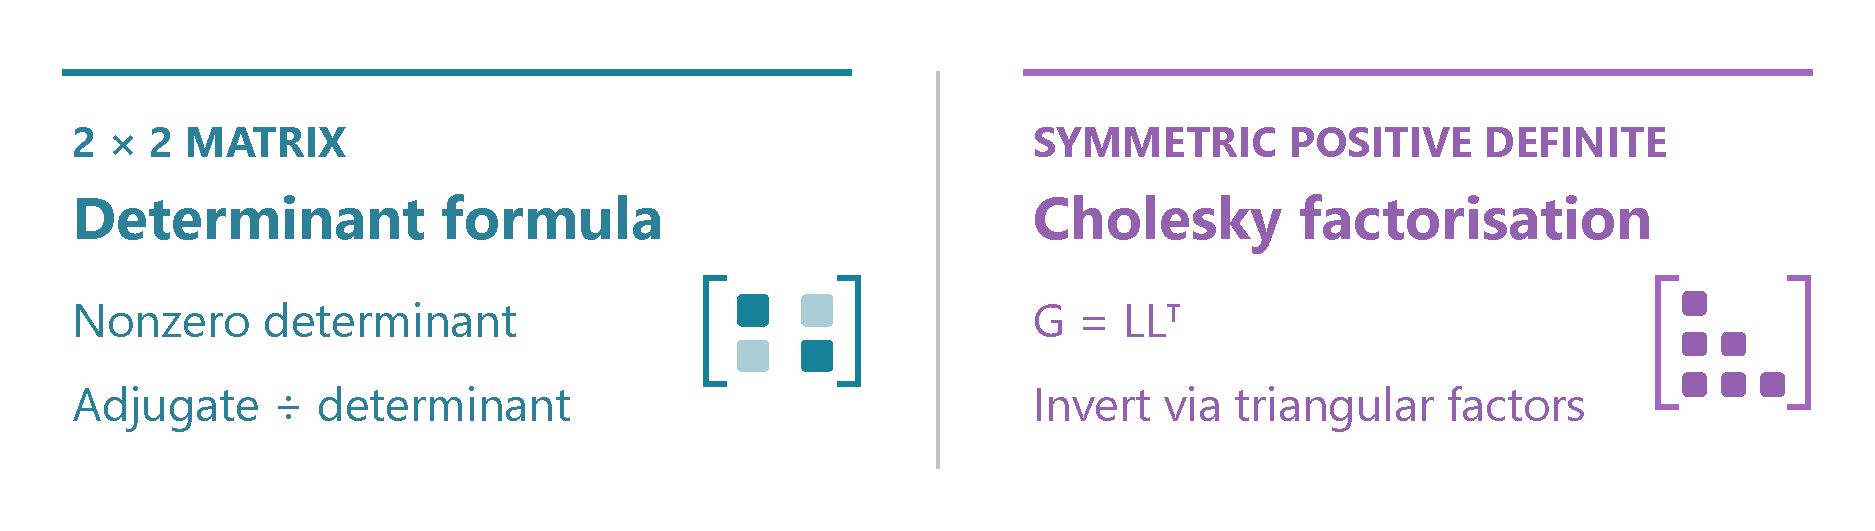
\includegraphics[width=\linewidth,height=.62\textheight,keepaspectratio]{asset-6eb85961665035502cf467fdb7020e2480fd5c0a3a60de477f61f2368d4a2022.pdf}\end{center}

\medskip

\par\medskip
\Needspace{10cm}
\refstepcounter{figure}\label{material-1162128eeba6878dafc3a5332d4b993e9a688d1f1463319c5a274caafef1b3e7}
\noindent\textbf{Fig.~\ref*{material-1162128eeba6878dafc3a5332d4b993e9a688d1f1463319c5a274caafef1b3e7}.} Michigan: 2 \ensuremath{\times} 2 inverse\par\nopagebreak
\noindent\href{https://sph.umich.edu/biostat/biostart/matrix\_inverse.html}{Michigan: 2 \ensuremath{\times} 2 inverse}\par
\nolinkurl{https://sph.umich.edu/biostat/biostart/matrix\_inverse.html}\par

\medskip

\par\medskip
\Needspace{10cm}
\refstepcounter{figure}\label{material-191900f793e247a2468a3ffb423595b7333b0e7fc6c83465cc8deef921c4ac4c}
\noindent\textbf{Fig.~\ref*{material-191900f793e247a2468a3ffb423595b7333b0e7fc6c83465cc8deef921c4ac4c}.} LAPACK: Cholesky inverse\par\nopagebreak
\noindent\href{https://www.netlib.org/lapack/explore-html/d4/d12/group\_\_potri\_gaced925926290482532c433f73b30b9f1.html}{LAPACK: Cholesky inverse}\par
\nolinkurl{https://www.netlib.org/lapack/explore-html/d4/d12/group\_\_potri\_gaced925926290482532c433f73b30b9f1.html}\par

\medskip

\clearpage
\section{From the formula to fitted models}
\textbf{Build the drift design and response}


Starting from the five readings in \hyperref[material-0cbd8025474be43ec999bee5b494a4a7786a19b561b67923fea96c6f1109b2da]{Fig.~\ref*{material-0cbd8025474be43ec999bee5b494a4a7786a19b561b67923fea96c6f1109b2da}}, \hyperref[material-29e4a576caf471eb7180f8a62cc9e5a5047be3484f49ffacafd9339304fc3a0c]{Fig.~\ref*{material-29e4a576caf471eb7180f8a62cc9e5a5047be3484f49ffacafd9339304fc3a0c}} lists the rows of \(X\) and \(y\) together. Pair the intercept column with itself to count five observations. Its product with the time column is \(0+1+2+3+4=10\), and the time column with itself gives \(0^2+1^2+2^2+3^2+4^2=30\). These fill \(X^\top X\). For \(X^\top y\), the intercept pairs with the readings to give their sum, 25 mV. The time column weights those readings by 0 through 4 min, giving 69.9 min\ensuremath{\cdot}mV.


\par\medskip
\Needspace{10cm}
\refstepcounter{figure}\label{material-29e4a576caf471eb7180f8a62cc9e5a5047be3484f49ffacafd9339304fc3a0c}
\noindent\textbf{Fig.~\ref*{material-29e4a576caf471eb7180f8a62cc9e5a5047be3484f49ffacafd9339304fc3a0c}.} Build X\ensuremath{{}^{\mathsf T}}X and X\ensuremath{{}^{\mathsf T}}y from the drift measurements\par\nopagebreak
\begin{center}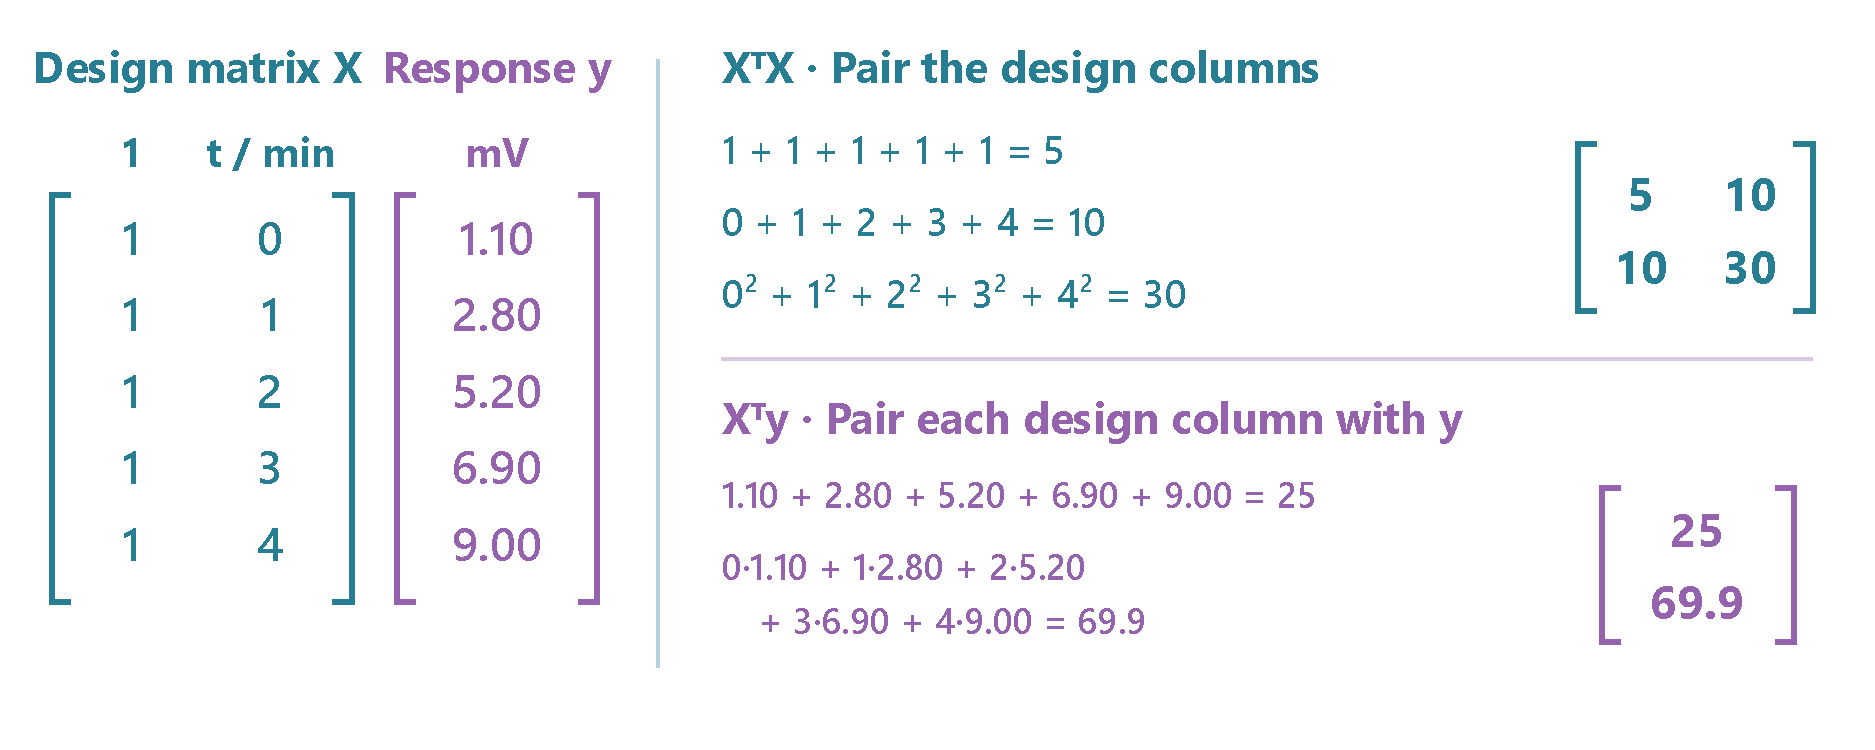
\includegraphics[width=\linewidth,height=.62\textheight,keepaspectratio]{asset-2d09585dfcc263e0ca412581e0bdb6c1a1836fa2d7237f32e70cc6a84f0b68df.pdf}\end{center}

\medskip

\textbf{Back to the detector: fit the drift line}


Substitute the products from \hyperref[material-29e4a576caf471eb7180f8a62cc9e5a5047be3484f49ffacafd9339304fc3a0c]{Fig.~\ref*{material-29e4a576caf471eb7180f8a62cc9e5a5047be3484f49ffacafd9339304fc3a0c}} in \hyperref[material-6c52e26e3cca426cb4a8c12c4a7ebb43b7ad5e355532b2802e095d4e4a6cbada]{Eq.~\ref*{material-6c52e26e3cca426cb4a8c12c4a7ebb43b7ad5e355532b2802e095d4e4a6cbada}}. The determinant is \(5\cdot30-10^2=50\). Multiplying the inverse by \(X^\top y\) gives an intercept of 1.02 mV and a slope of 1.99 mV/min.


\par\medskip
\noindent\begin{minipage}{\linewidth}
\refstepcounter{equation}\label{material-6c52e26e3cca426cb4a8c12c4a7ebb43b7ad5e355532b2802e095d4e4a6cbada}
\noindent\textbf{Eq.~\ref*{material-6c52e26e3cca426cb4a8c12c4a7ebb43b7ad5e355532b2802e095d4e4a6cbada}.} Back to the detector: fit the drift line\par\nopagebreak
\begin{center}\begin{adjustbox}{max width=\linewidth}$\displaystyle \begin{aligned}\widehat\beta&=\underbrace{\textcolor{teal}{\begin{bmatrix}5&10\\10&30\end{bmatrix}}^{\textcolor{brown}{-1}}}_{\text{inverse of }X^{\mathsf T}X}\quad\underbrace{\textcolor{purple}{\begin{bmatrix}25\\69.9\end{bmatrix}}}_{X^{\mathsf T}y}\\[.7em]&=\textcolor{brown}{\frac{1}{50}\begin{bmatrix}30&-10\\-10&5\end{bmatrix}}\textcolor{purple}{\begin{bmatrix}25\\69.9\end{bmatrix}}=\begin{bmatrix}1.02\\1.99\end{bmatrix}\end{aligned}$\end{adjustbox}\end{center}

\par\noindent\textbf{Symbols}

\par\noindent\textbf{\(+,-,=,\cdot\)} Plus adds, minus subtracts, equals asserts equality; juxtaposition, a centred dot or \ensuremath{\times} between numerical entries multiplies. Parentheses group terms; brackets arrange matrix entries. Bare numerical constants are dimensionless unless the stated measurement coordinates give units.

\par\noindent\textbf{\(X\)} Design matrix: 5 rows (observations), 2 columns (constant and time) for the drift line. The constant column is dimensionless; the time column has unit min.

\par\noindent\textbf{\(\beta,\widehat\beta\)} Coefficient column ordered intercept then slope. Hats mark the least-squares solution: entries have units mV and mV/min respectively. Different coefficient entries need not share one unit.

\par\noindent\textbf{\(y,\widehat y,e\)} Observed, fitted and residual columns of length 5, each in mV; e = y \ensuremath{-} ŷ. Superscript T transposes a column into a row.

\par\noindent\textbf{\({}^{-1}\)} Matrix inverse, not entrywise reciprocal: for a nonsingular square matrix, multiplication on either side gives the identity.

\par\noindent\textbf{\({}^{\mathsf T}\)} Transpose: swap rows and columns. (AB)\ensuremath{{}^{\mathsf T}} reverses the multiplication order to B\ensuremath{{}^{\mathsf T}}A\ensuremath{{}^{\mathsf T}}.

\end{minipage}\par
\medskip

\textbf{Back to the detector: predict the signal at 2.5 min}


Return to the five detector readings from \hyperref[material-0cbd8025474be43ec999bee5b494a4a7786a19b561b67923fea96c6f1109b2da]{Fig.~\ref*{material-0cbd8025474be43ec999bee5b494a4a7786a19b561b67923fea96c6f1109b2da}}. The least-squares line shown in \hyperref[material-f4966e0974e501f25636c0dc06f8fc5c39c5a6a2d5760824e55f2b0fd369ae2d]{Fig.~\ref*{material-f4966e0974e501f25636c0dc06f8fc5c39c5a6a2d5760824e55f2b0fd369ae2d}} is \(\widehat y=1.02+1.99t\), with \(t\) in minutes and \(\widehat y\) in millivolts. Evaluating it at 2.5 min gives \(1.02+1.99\cdot2.5=5.995\) mV. The requested time falls between two observed times, so this is interpolation.


\par\medskip
\Needspace{10cm}
\refstepcounter{figure}\label{material-f4966e0974e501f25636c0dc06f8fc5c39c5a6a2d5760824e55f2b0fd369ae2d}
\noindent\textbf{Fig.~\ref*{material-f4966e0974e501f25636c0dc06f8fc5c39c5a6a2d5760824e55f2b0fd369ae2d}.} Fitted detector drift and interpolation at 2.5 min\par\nopagebreak
\begin{center}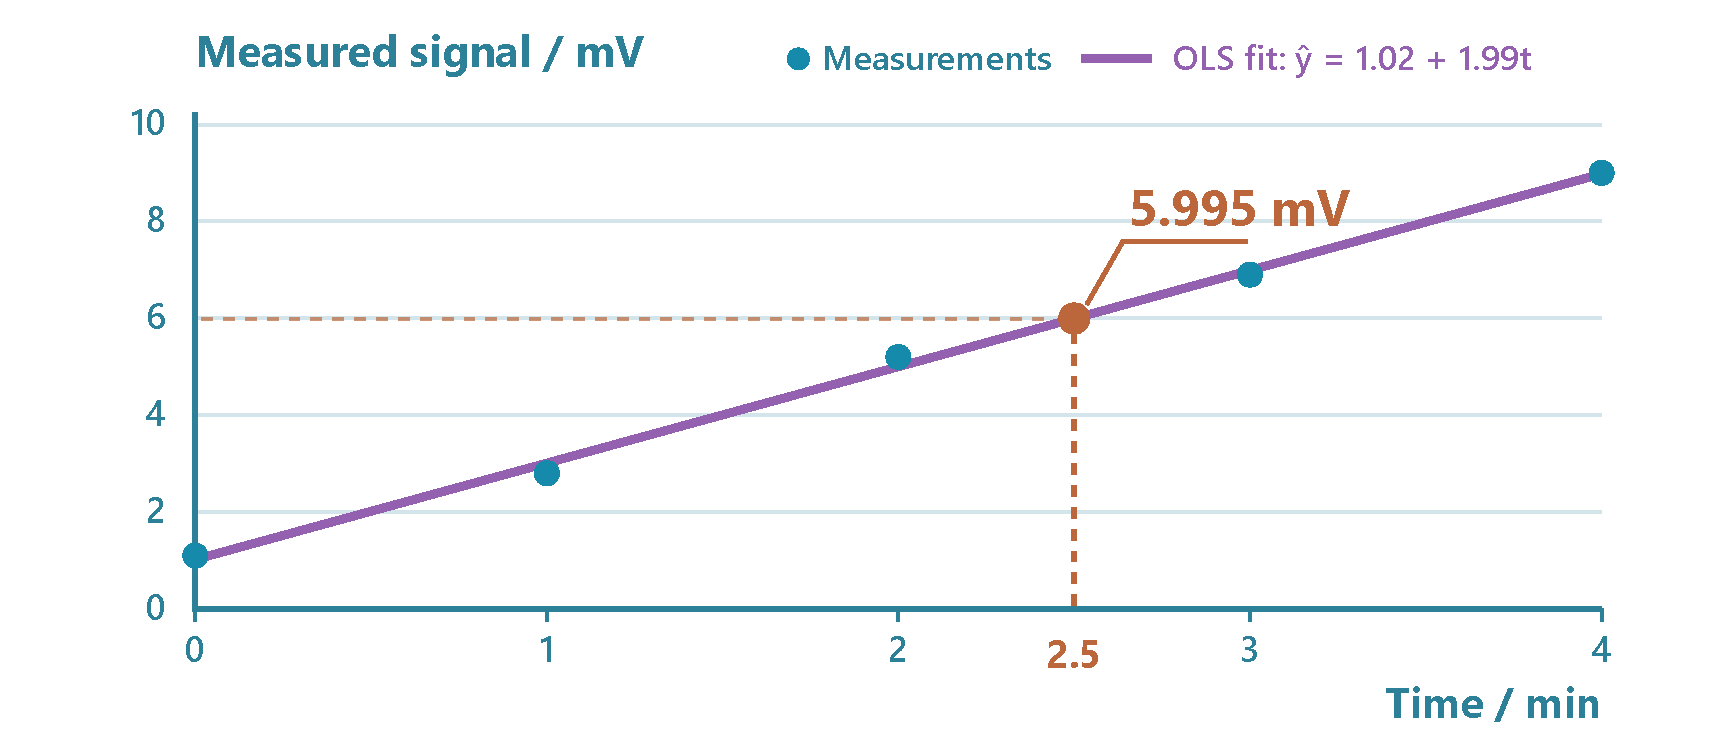
\includegraphics[width=\linewidth,height=.62\textheight,keepaspectratio]{asset-db1596c6de085c793e156b02c8b4f8cda98189fc5afcd11c5d505fbdbdf75fea.pdf}\end{center}

\medskip

\textbf{A heating ramp with a changing rate}


The temperature was recorded once a minute for four minutes. The least-squares straight line in \hyperref[material-1b8c48220996b387bc8110b728f8a91f67c6312c23af8ac73aedc4dad19e1afb]{Fig.~\ref*{material-1b8c48220996b387bc8110b728f8a91f67c6312c23af8ac73aedc4dad19e1afb}} assumes a constant change per minute. Its residuals are positive at both ends and negative in the middle. That systematic pattern suggests that the temperature rises faster later in the run.


\par\medskip
\Needspace{10cm}
\refstepcounter{figure}\label{material-1b8c48220996b387bc8110b728f8a91f67c6312c23af8ac73aedc4dad19e1afb}
\noindent\textbf{Fig.~\ref*{material-1b8c48220996b387bc8110b728f8a91f67c6312c23af8ac73aedc4dad19e1afb}.} Where does a straight line miss the heating data?\par\nopagebreak
\begin{center}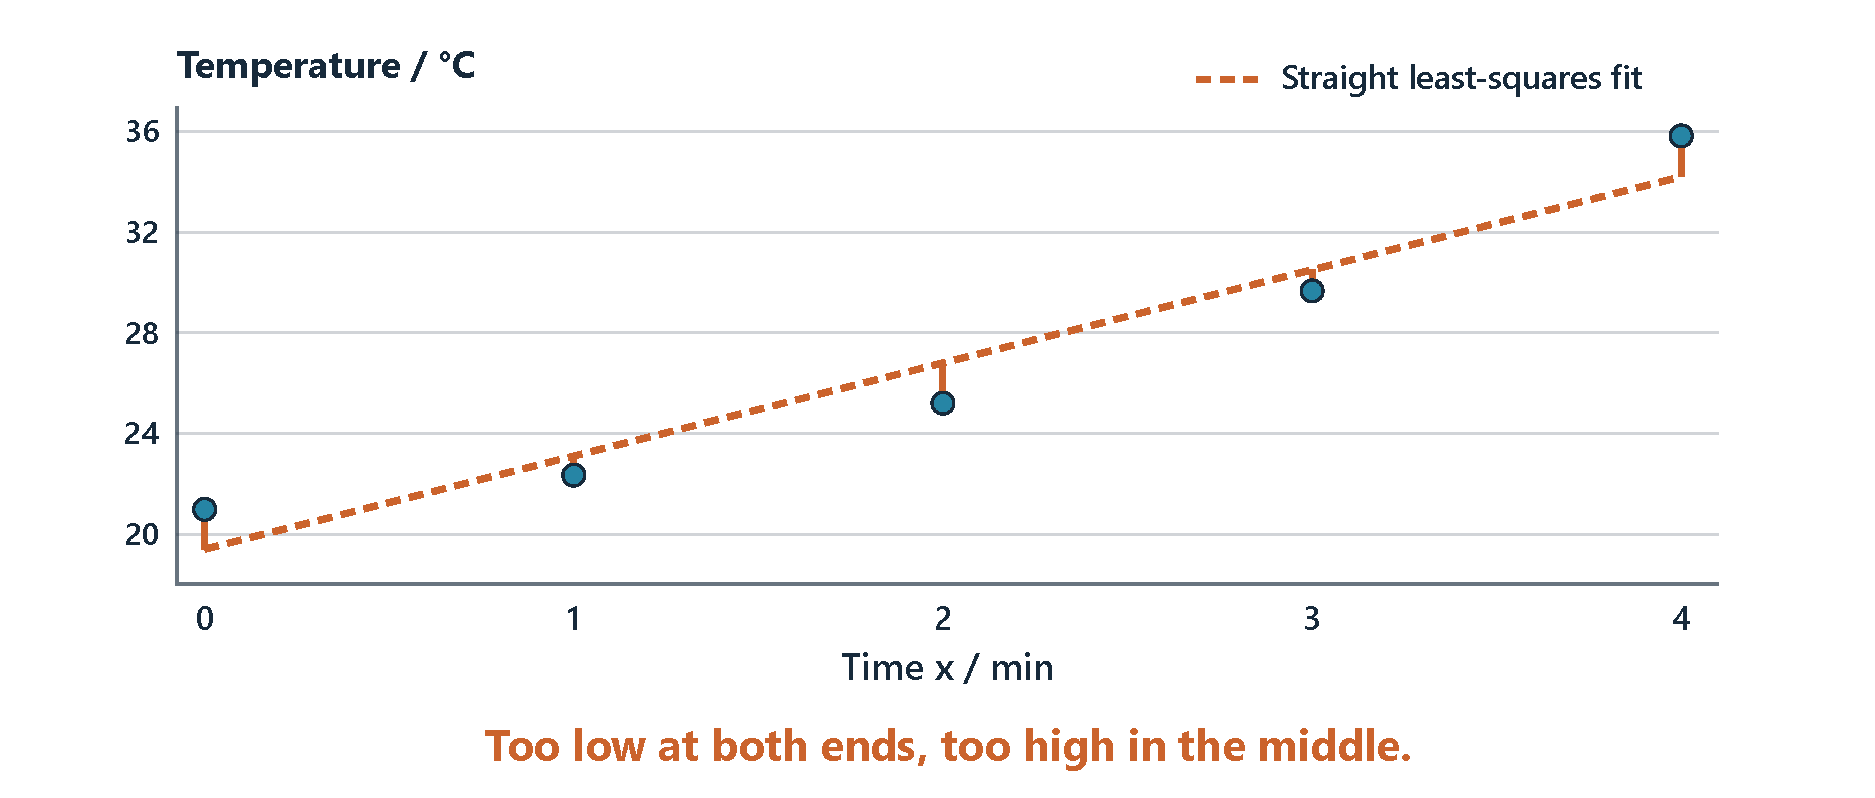
\includegraphics[width=\linewidth,height=.62\textheight,keepaspectratio]{asset-a70237929e1d57612378d0a81e82b5da6a32f77ec34acaccfd1d69441e950d3c.pdf}\end{center}

\medskip

\textbf{Add a column for squared time}


In \hyperref[material-6b7c42b27eda656bbaa79402fb33241e055f3626d59c04c05ff2dfbd9cc4ebe1]{Fig.~\ref*{material-6b7c42b27eda656bbaa79402fb33241e055f3626d59c04c05ff2dfbd9cc4ebe1}}, each row pairs one observation with three known inputs. The intercept column contains ones. The next column contains elapsed time \(x\) in minutes, and the third contains its square \(x^2\) in minutes squared. At 3 min, for example, the inputs are 1, 3 and 9, and the observed response is 29.66 °C. The same ordinary least-squares procedure estimates three coefficients. The fitted coefficients are 21.00 °C for the intercept, 0.50 °C/min for time and 0.80 °C/min\ensuremath{{}^2} for squared time. The sum of squared residuals falls from 8.964 °C\ensuremath{{}^2} for the line to 0.004 °C\ensuremath{{}^2} for the quadratic fit on these observations.


\par\medskip
\Needspace{10cm}
\refstepcounter{figure}\label{material-6b7c42b27eda656bbaa79402fb33241e055f3626d59c04c05ff2dfbd9cc4ebe1}
\noindent\textbf{Fig.~\ref*{material-6b7c42b27eda656bbaa79402fb33241e055f3626d59c04c05ff2dfbd9cc4ebe1}.} Build and fit a quadratic heating model\par\nopagebreak
\begin{center}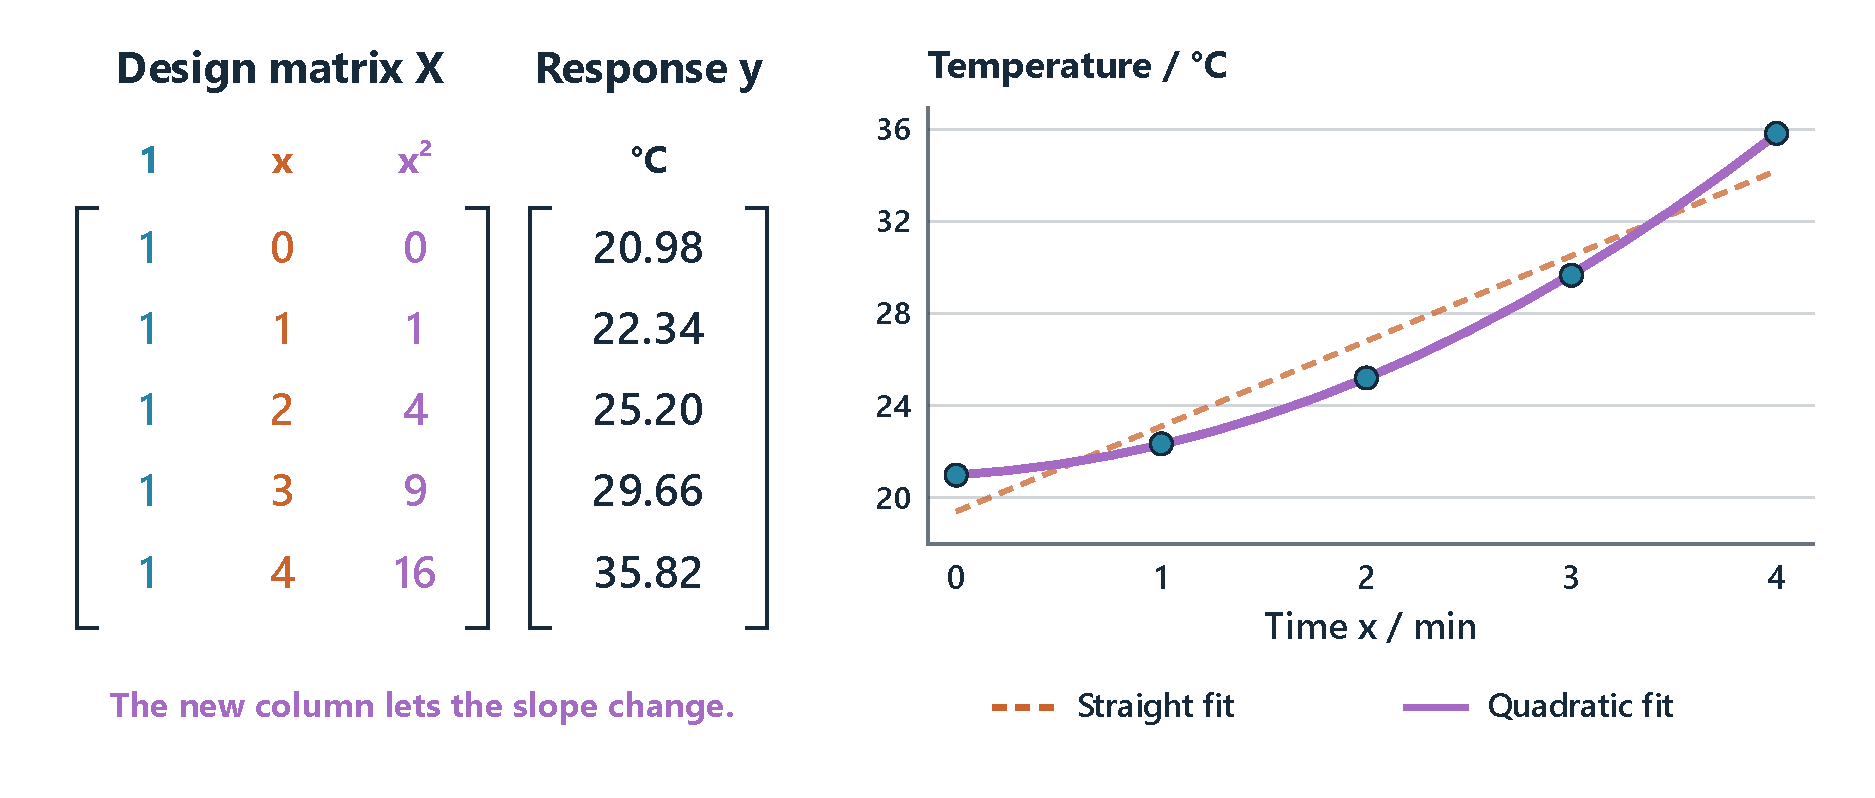
\includegraphics[width=\linewidth,height=.62\textheight,keepaspectratio]{asset-18b461f47684c0d9ebbeaefaef2925b5b59fce6ea9bc6c6868b6914f94f97cb1.pdf}\end{center}

\medskip

\textbf{An exponential decay on two scales}


\hyperref[material-f5b6760bc47e33af458226304e72a19db90766c2f910188be1256683265f2a8e]{Fig.~\ref*{material-f5b6760bc47e33af458226304e72a19db90766c2f910188be1256683265f2a8e}} starts with five tracer concentrations in mg/L. The first one-minute drop is about 5.65 mg/L, while the last is only about 1.67 mg/L. If a similar fraction of the tracer remains after each minute, the same relative loss translates into a smaller absolute drop as the concentration declines.


\par\medskip
\Needspace{10cm}
\refstepcounter{figure}\label{material-f5b6760bc47e33af458226304e72a19db90766c2f910188be1256683265f2a8e}
\noindent\textbf{Fig.~\ref*{material-f5b6760bc47e33af458226304e72a19db90766c2f910188be1256683265f2a8e}.} How does the concentration fall over time?\par\nopagebreak
\begin{center}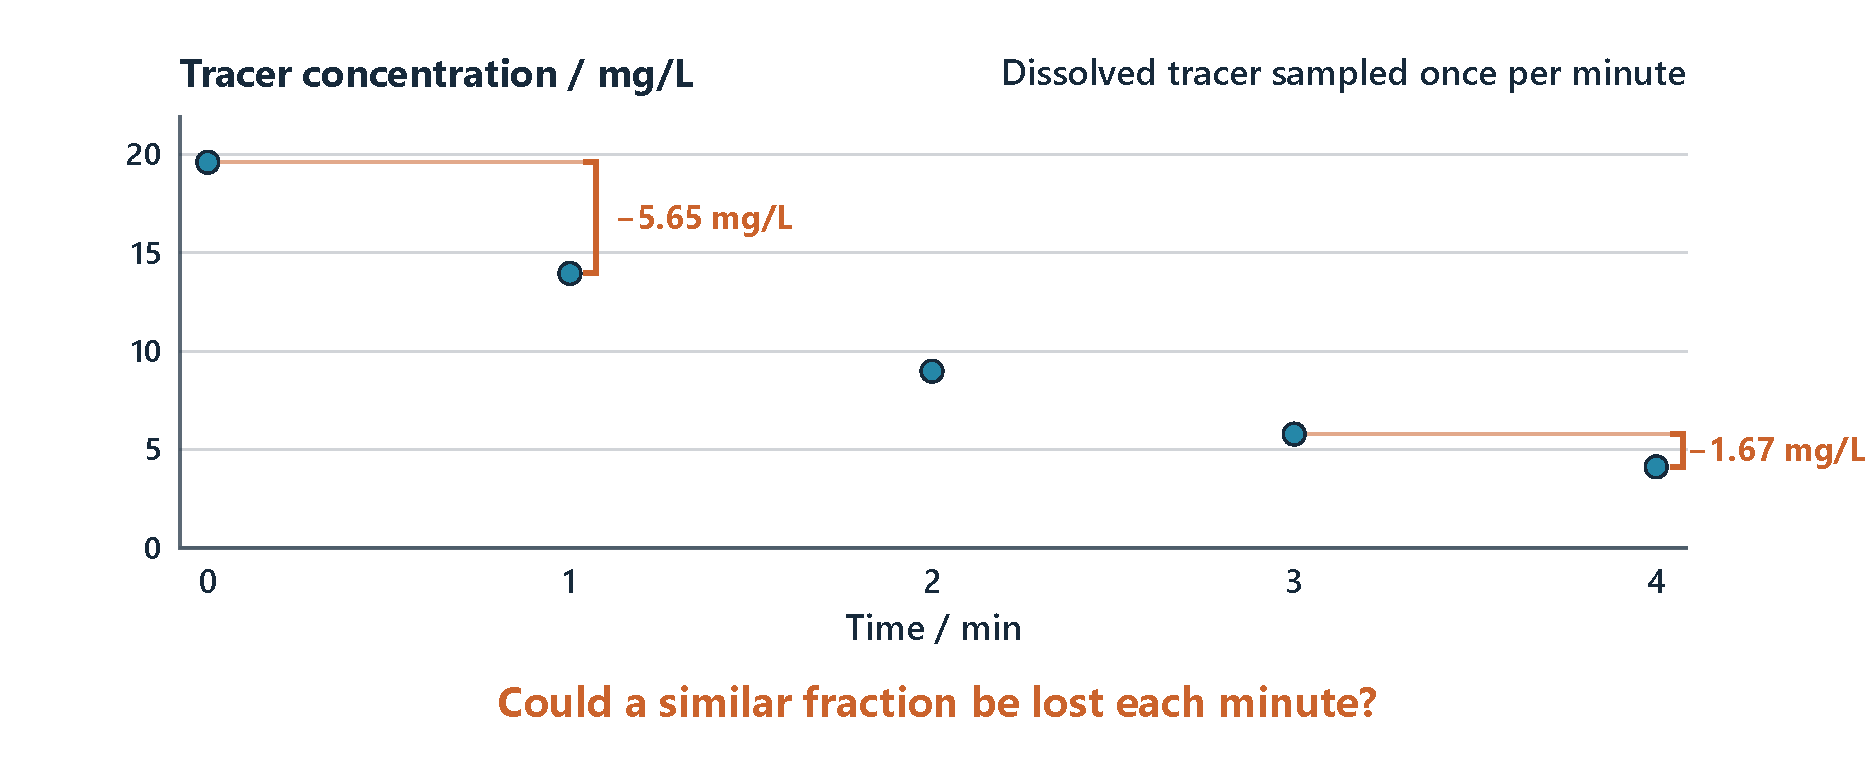
\includegraphics[width=\linewidth,height=.62\textheight,keepaspectratio]{asset-621b47d93428899f3b5c03cfcfe3ced0973d5b394ee1285a95faee2ed8c77837.pdf}\end{center}

\medskip

The transformation in \hyperref[material-b55dee9b5fa107f70d1bec962fce5e844678d519315b9f4685e527e2d1d14597]{Eq.~\ref*{material-b55dee9b5fa107f70d1bec962fce5e844678d519315b9f4685e527e2d1d14597}} divides each positive measured concentration by the reference of 1 mg/L before taking its natural logarithm. Time stays in minutes. The difference between two consecutive logarithms is the logarithm of the ratio of their concentrations. A constant retention fraction therefore produces an equal step for each equal time interval.


\par\medskip
\noindent\begin{minipage}{\linewidth}
\refstepcounter{equation}\label{material-b55dee9b5fa107f70d1bec962fce5e844678d519315b9f4685e527e2d1d14597}
\noindent\textbf{Eq.~\ref*{material-b55dee9b5fa107f70d1bec962fce5e844678d519315b9f4685e527e2d1d14597}.} Why take the log of the concentration?\par\nopagebreak
\begin{center}\begin{adjustbox}{max width=\linewidth}$\displaystyle \begin{aligned} z_i &= \ln\!\left(\frac{C_i}{C_*}\right) & z_1 &\approx \ln\!\left(\frac{19.60}{1.00}\right) \approx 2.98 \\[.65em] z_{i+1}-z_i &= \ln\!\left(\frac{C_{i+1}}{C_i}\right) && \end{aligned}$\end{adjustbox}\end{center}

\par\noindent\textbf{Symbols}

\par\noindent\textbf{\(=,-,\approx\)} Equals, subtraction and approximately equals. Fraction bars divide. In the example, 19.60 and 1.00 are concentrations in the same unit.

\par\noindent\textbf{\(C_i,C_{i+1},C_*\)} Current and next positive concentrations in mg/L. The reference C* is 1 mg/L, so the ratios have no unit.

\par\noindent\textbf{\(\ln\)} Natural logarithm of a positive dimensionless ratio.

\par\noindent\textbf{\(z_i,z_{i+1},z_1\)} Unitless log responses. Index i marks the current sample, i+1 the next and 1 the first.

\end{minipage}\par
\medskip

In \hyperref[material-d652b521a2486a8240f33fd88dc397fc7db1997646384f8f5f0524b901a57d26]{Fig.~\ref*{material-d652b521a2486a8240f33fd88dc397fc7db1997646384f8f5f0524b901a57d26}}, both panels show the same observations. The line in \hyperref[material-7354b0845c326c007133824f2a63278f221b0d436da64c8be94169ad493eeefb]{Eq.~\ref*{material-7354b0845c326c007133824f2a63278f221b0d436da64c8be94169ad493eeefb}} is fitted by ordinary least squares on the log scale, with an intercept of about 2.996 and a slope of \ensuremath{-}0.40 per minute. Apply the exponential in the second equation to the fitted log values to recover a curve in mg/L. Each minute the model retains about 67\% of the preceding concentration. The regression minimises squared errors on the log scale.


\par\medskip
\Needspace{10cm}
\refstepcounter{figure}\label{material-d652b521a2486a8240f33fd88dc397fc7db1997646384f8f5f0524b901a57d26}
\noindent\textbf{Fig.~\ref*{material-d652b521a2486a8240f33fd88dc397fc7db1997646384f8f5f0524b901a57d26}.} Fit a line, then return to mg/L\par\nopagebreak
\begin{center}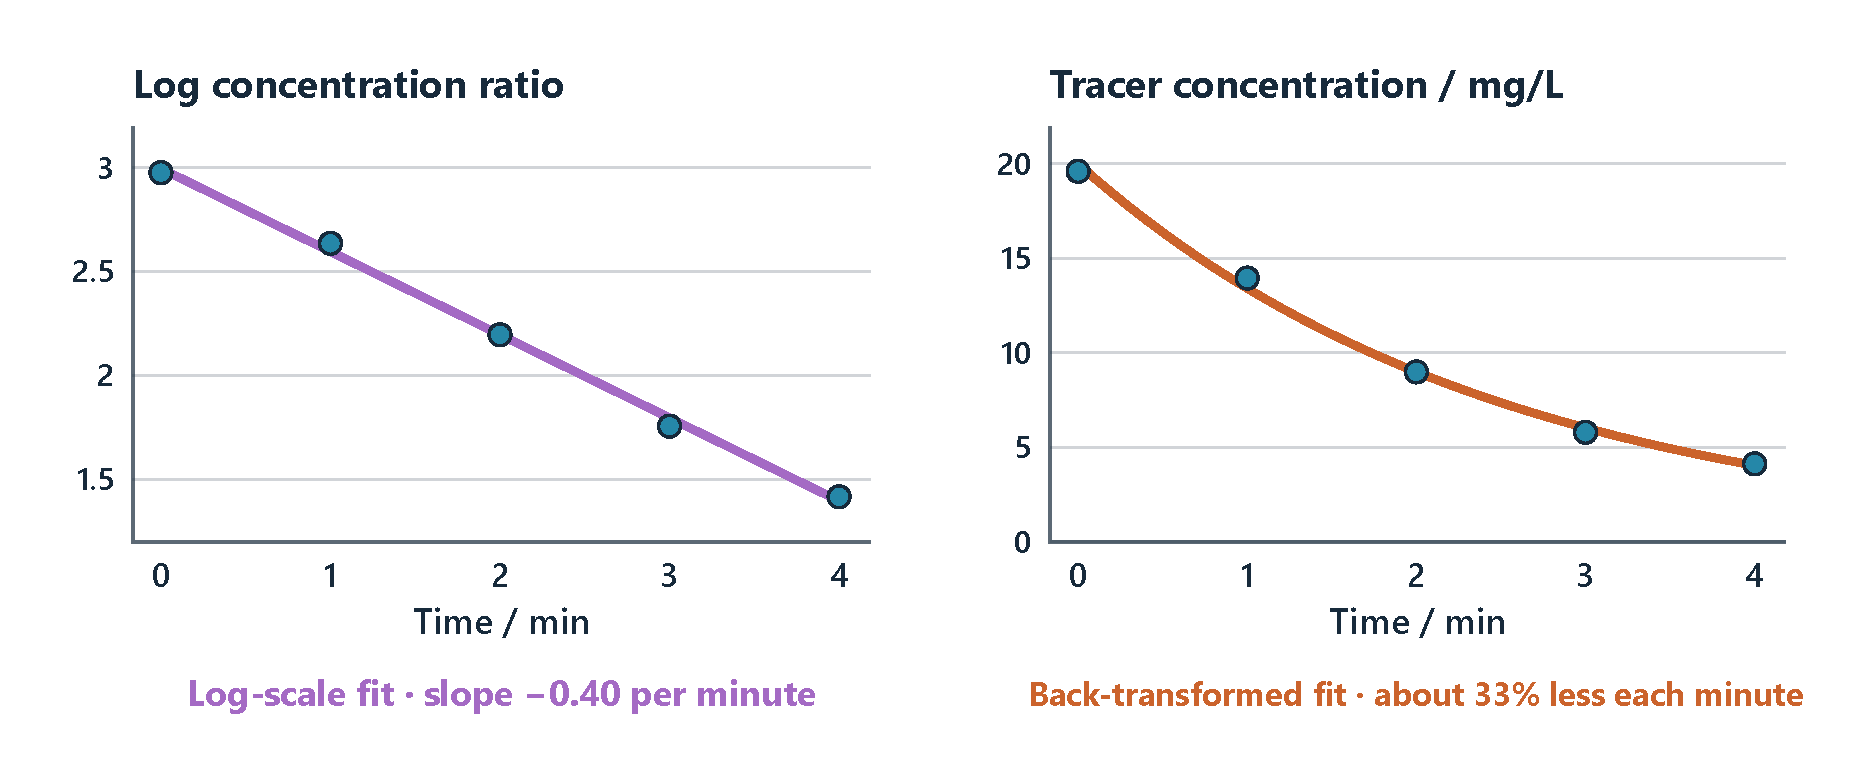
\includegraphics[width=\linewidth,height=.62\textheight,keepaspectratio]{asset-3e210f568f53cca750954ab0f2f23e6a396c8a94831737f147658795cc003638.pdf}\end{center}

\medskip

\par\medskip
\noindent\begin{minipage}{\linewidth}
\refstepcounter{equation}\label{material-7354b0845c326c007133824f2a63278f221b0d436da64c8be94169ad493eeefb}
\noindent\textbf{Eq.~\ref*{material-7354b0845c326c007133824f2a63278f221b0d436da64c8be94169ad493eeefb}.} Log-scale regression and back-transformation\par\nopagebreak
\begin{center}\begin{adjustbox}{max width=\linewidth}$\displaystyle \begin{aligned}\widehat z(t)&=\ln(20)-0.40\,\mathrm{min}^{-1}t\\[.5em]\widehat C(t)&=C_*\exp\!\bigl(\widehat z(t)\bigr)\\&=20\,\mathrm{mg/L}\,\exp\!\bigl(-0.40\,\mathrm{min}^{-1}t\bigr)\end{aligned}$\end{adjustbox}\end{center}

\par\noindent\textbf{Symbols}

\par\noindent\textbf{\(=,-,{}^{-1}\)} Equality and subtraction. A min\ensuremath{{}^-}\ensuremath{{}^1} unit means per minute. Adjacent factors multiply.

\par\noindent\textbf{\(C_*,t\)} Reference concentration of 1 mg/L and time in minutes. The log-scale intercept is ln(20); slope is \ensuremath{-}0.40 per minute.

\par\noindent\textbf{\(\ln,\exp\)} Natural logarithm and its inverse, the exponential. Both function arguments are dimensionless.

\par\noindent\textbf{\(\widehat z,\widehat C\)} Fitted log response (unitless) and fitted concentration (mg/L). Hats mark fitted values.

\end{minipage}\par
\medskip

\textbf{Multiple linear regression with two measured predictors}


\hyperref[material-b7550d93f20ee229a8d0613c51bde76ad20c4bef6250499db09635dbf994a06f]{Fig.~\ref*{material-b7550d93f20ee229a8d0613c51bde76ad20c4bef6250499db09635dbf994a06f}} shows six synthetic detector readings for three concentrations at two temperatures. Each row pairs both settings with one response. The design columns contain ones, the measured concentration, and the measured temperature in °C. As in earlier examples, ordinary least squares estimates all coefficients at once.


\par\medskip
\Needspace{10cm}
\refstepcounter{figure}\label{material-b7550d93f20ee229a8d0613c51bde76ad20c4bef6250499db09635dbf994a06f}
\noindent\textbf{Fig.~\ref*{material-b7550d93f20ee229a8d0613c51bde76ad20c4bef6250499db09635dbf994a06f}.} Multiple linear regression: two predictors\par\nopagebreak
\begin{center}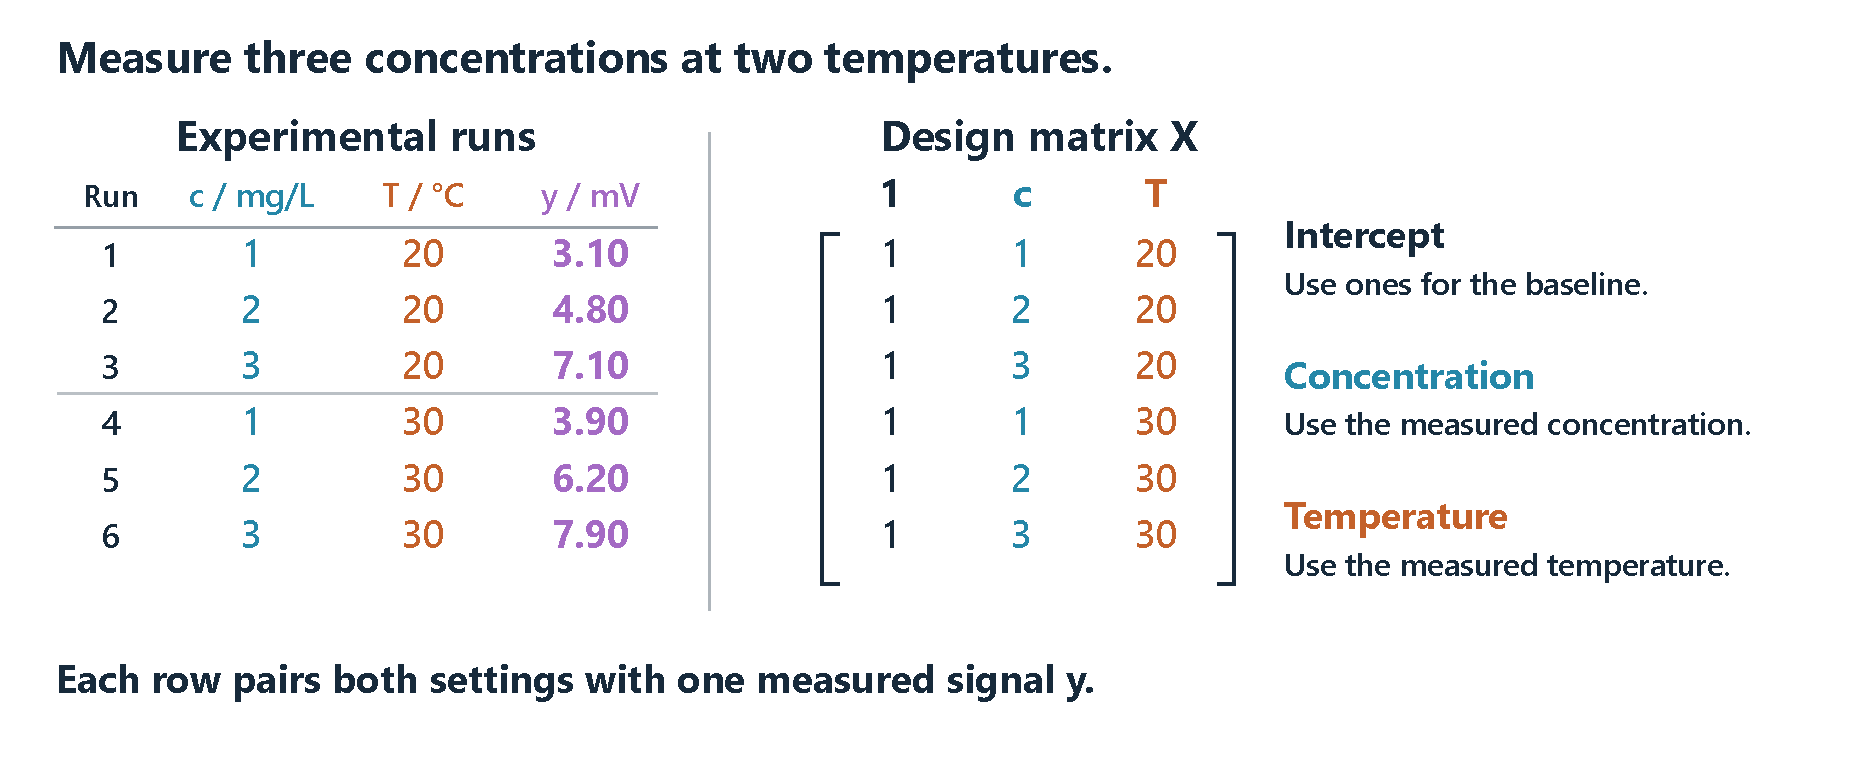
\includegraphics[width=\linewidth,height=.62\textheight,keepaspectratio]{asset-8ab41cb3bf40ef4585da0da87a02aa5ef658aff05a187843a097addf960c539f.pdf}\end{center}

\medskip

\hyperref[material-a4ebf797b4534a4bf0465dac15c80e9d6abddf6a0cb9f734a0dd46ec2bf4c541]{Fig.~\ref*{material-a4ebf797b4534a4bf0465dac15c80e9d6abddf6a0cb9f734a0dd46ec2bf4c541}} starts from the same six rows. Apply \hyperref[material-7b228cf9ca6448dc0f6261b3b67283218661c4d8cf761a03cdd41c142b56ea7b]{Eq.~\ref*{material-7b228cf9ca6448dc0f6261b3b67283218661c4d8cf761a03cdd41c142b56ea7b}} by multiplying entries in corresponding rows and adding the products. For example, pairing concentration with temperature gives \((20+30)(1+2+3)=300\). This value appears in both symmetric positions of \(X^\top X\). For \(X^\top y\), the ones sum the six signals to 33, the concentrations weight them to give 74, and the measured temperatures weight them to give 840.


\par\medskip
\Needspace{10cm}
\refstepcounter{figure}\label{material-a4ebf797b4534a4bf0465dac15c80e9d6abddf6a0cb9f734a0dd46ec2bf4c541}
\noindent\textbf{Fig.~\ref*{material-a4ebf797b4534a4bf0465dac15c80e9d6abddf6a0cb9f734a0dd46ec2bf4c541}.} Build X\ensuremath{{}^{\mathsf T}}X and X\ensuremath{{}^{\mathsf T}}y from the six runs\par\nopagebreak
\begin{center}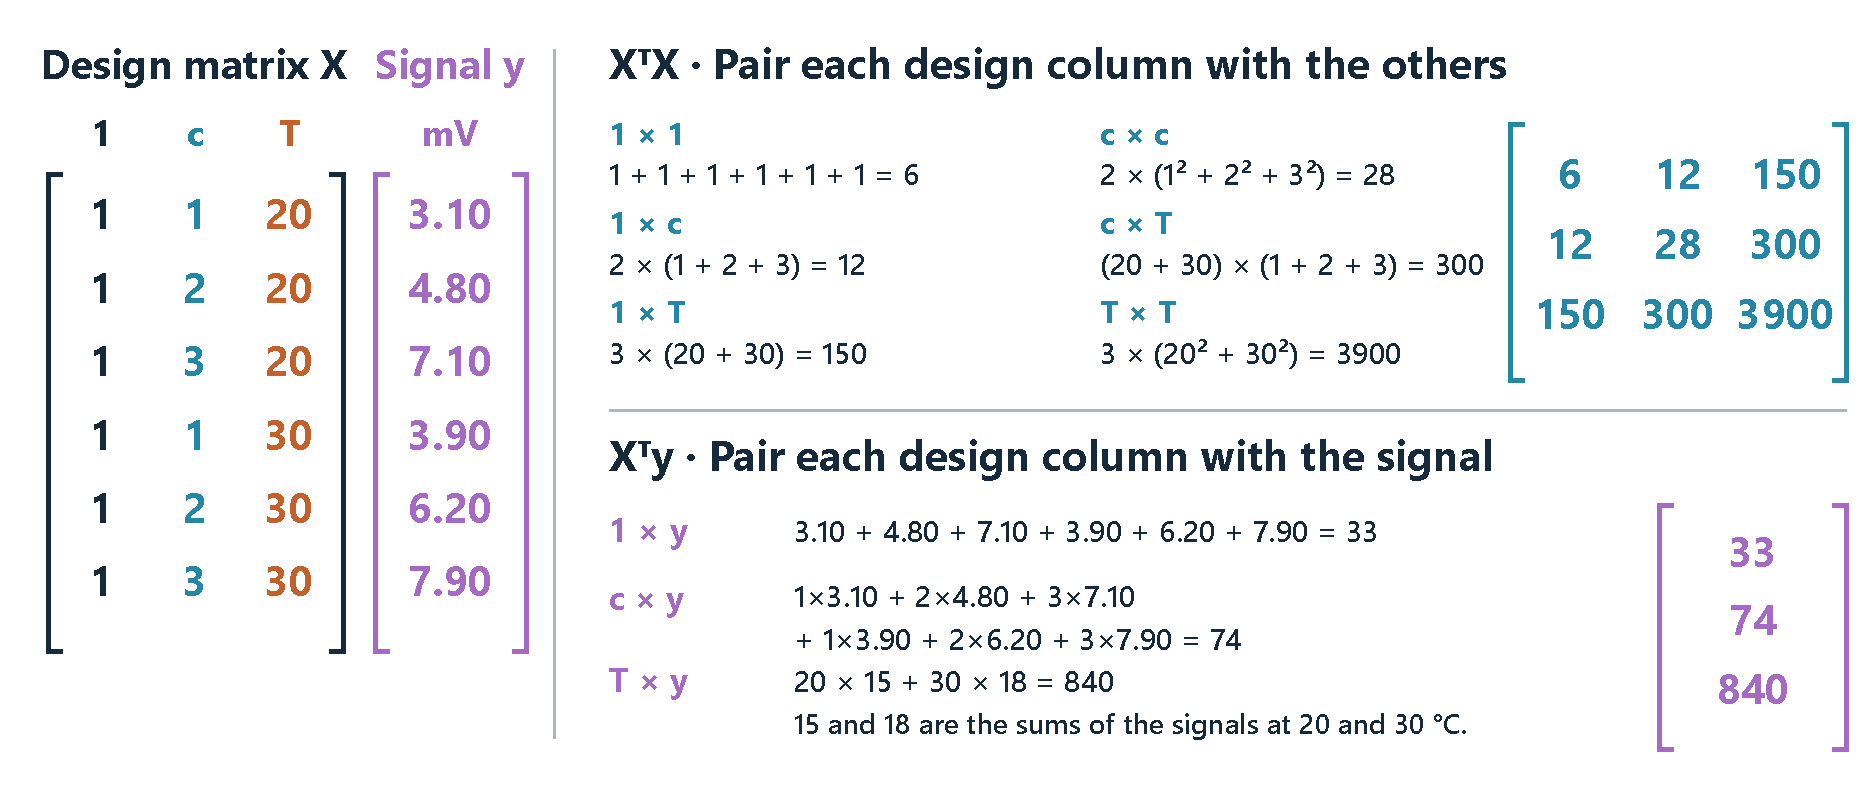
\includegraphics[width=\linewidth,height=.62\textheight,keepaspectratio]{asset-cc7886e8a20843b4267fb30d898b935d360331852fb35cec649867a6cf22e5a2.pdf}\end{center}

\medskip

\par\medskip
\noindent\begin{minipage}{\linewidth}
\refstepcounter{equation}\label{material-7b228cf9ca6448dc0f6261b3b67283218661c4d8cf761a03cdd41c142b56ea7b}
\noindent\textbf{Eq.~\ref*{material-7b228cf9ca6448dc0f6261b3b67283218661c4d8cf761a03cdd41c142b56ea7b}.} Compute each product entry\par\nopagebreak
\begin{center}\begin{adjustbox}{max width=\linewidth}$\displaystyle \begin{aligned}(X^{\mathsf T}X)_{jk}&=\sum_{i=1}^{6}X_{ij}X_{ik}\\[.45em](X^{\mathsf T}y)_j&=\sum_{i=1}^{6}X_{ij}y_i\end{aligned}$\end{adjustbox}\end{center}

\par\noindent\textbf{Symbols}

\par\noindent\textbf{\(X,y\)} Design matrix with six rows and columns for ones, concentration c (mg/L), and measured temperature T (°C). The six detector signals y are measured in mV.

\par\noindent\textbf{\(X_{ij},X_{ik},y_i\)} Values from the indicated columns in run i and its measured signal. Parenthesised products with subscripts denote entries of the result.

\par\noindent\textbf{\(i,j,k\)} Row i identifies one of the six runs. Columns j and k identify one of the three predictors including the column of ones.

\par\noindent\textbf{\({}^{\mathsf T},\sum,=\)} Transpose swaps rows and columns. The sum runs over the six runs. Adjacent factors multiply. The equals sign gives the resulting entry.

\end{minipage}\par
\medskip

In \hyperref[material-c7bcd8df3905fc339dee04263f4bc7e2444f6641f9145cf0aeea5109b80684f9]{Eq.~\ref*{material-c7bcd8df3905fc339dee04263f4bc7e2444f6641f9145cf0aeea5109b80684f9}}, substitute the two products in the coefficient formula. Multiplying by the inverse yields \ensuremath{-}1.00 mV for the intercept, 2.00 mV per mg/L for the concentration slope, and 0.10 mV per °C for the temperature slope. The intercept is the model prediction at zero concentration and 0 °C, outside the measured settings.


\par\medskip
\noindent\begin{minipage}{\linewidth}
\refstepcounter{equation}\label{material-c7bcd8df3905fc339dee04263f4bc7e2444f6641f9145cf0aeea5109b80684f9}
\noindent\textbf{Eq.~\ref*{material-c7bcd8df3905fc339dee04263f4bc7e2444f6641f9145cf0aeea5109b80684f9}.} Substitute the products to get three coefficients\par\nopagebreak
\begin{center}\begin{adjustbox}{max width=\linewidth}$\displaystyle \begin{aligned}\widehat\beta&=(X^{\mathsf T}X)^{-1}X^{\mathsf T}y\\[.6em]&=\textcolor{teal}{\begin{bmatrix}6&12&150\\12&28&300\\150&300&3900\end{bmatrix}}^{-1}\textcolor{purple}{\begin{bmatrix}33\\74\\840\end{bmatrix}}=\begin{bmatrix}-1.00\\2.00\\0.10\end{bmatrix}\end{aligned}$\end{adjustbox}\end{center}

\par\noindent\textbf{Symbols}

\par\noindent\textbf{\(X,y\)} The six-run design matrix and measured detector signals in mV. Design columns are ones, concentration in mg/L, and measured temperature in °C.

\par\noindent\textbf{\(\widehat\beta\)} Fitted coefficients in this order: intercept (mV), concentration slope (mV per mg/L), and temperature slope (mV per °C).

\par\noindent\textbf{\({}^{\mathsf T},{}^{-1},=\)} Transpose swaps rows and columns, \ensuremath{-}1 denotes the inverse of the whole square matrix, and equals gives the evaluated expression. Adjacent matrices or vectors multiply.

\end{minipage}\par
\medskip

In \hyperref[material-43a2db282318cd1d955dc5623b4079389b13dda467f425b3da814ed3915f05a4]{Fig.~\ref*{material-43a2db282318cd1d955dc5623b4079389b13dda467f425b3da814ed3915f05a4}}, the fitted signal forms a plane above the two predictor axes. Fixing temperature at 20 or 30 °C cuts that plane along a straight line. Both cuts have the same concentration slope because the model uses a single concentration coefficient. The six dots are the measured signals at the corresponding concentration and temperature.


\par\medskip
\Needspace{10cm}
\refstepcounter{figure}\label{material-43a2db282318cd1d955dc5623b4079389b13dda467f425b3da814ed3915f05a4}
\noindent\textbf{Fig.~\ref*{material-43a2db282318cd1d955dc5623b4079389b13dda467f425b3da814ed3915f05a4}.} Where do the two fitted lines come from?\par\nopagebreak
\begin{center}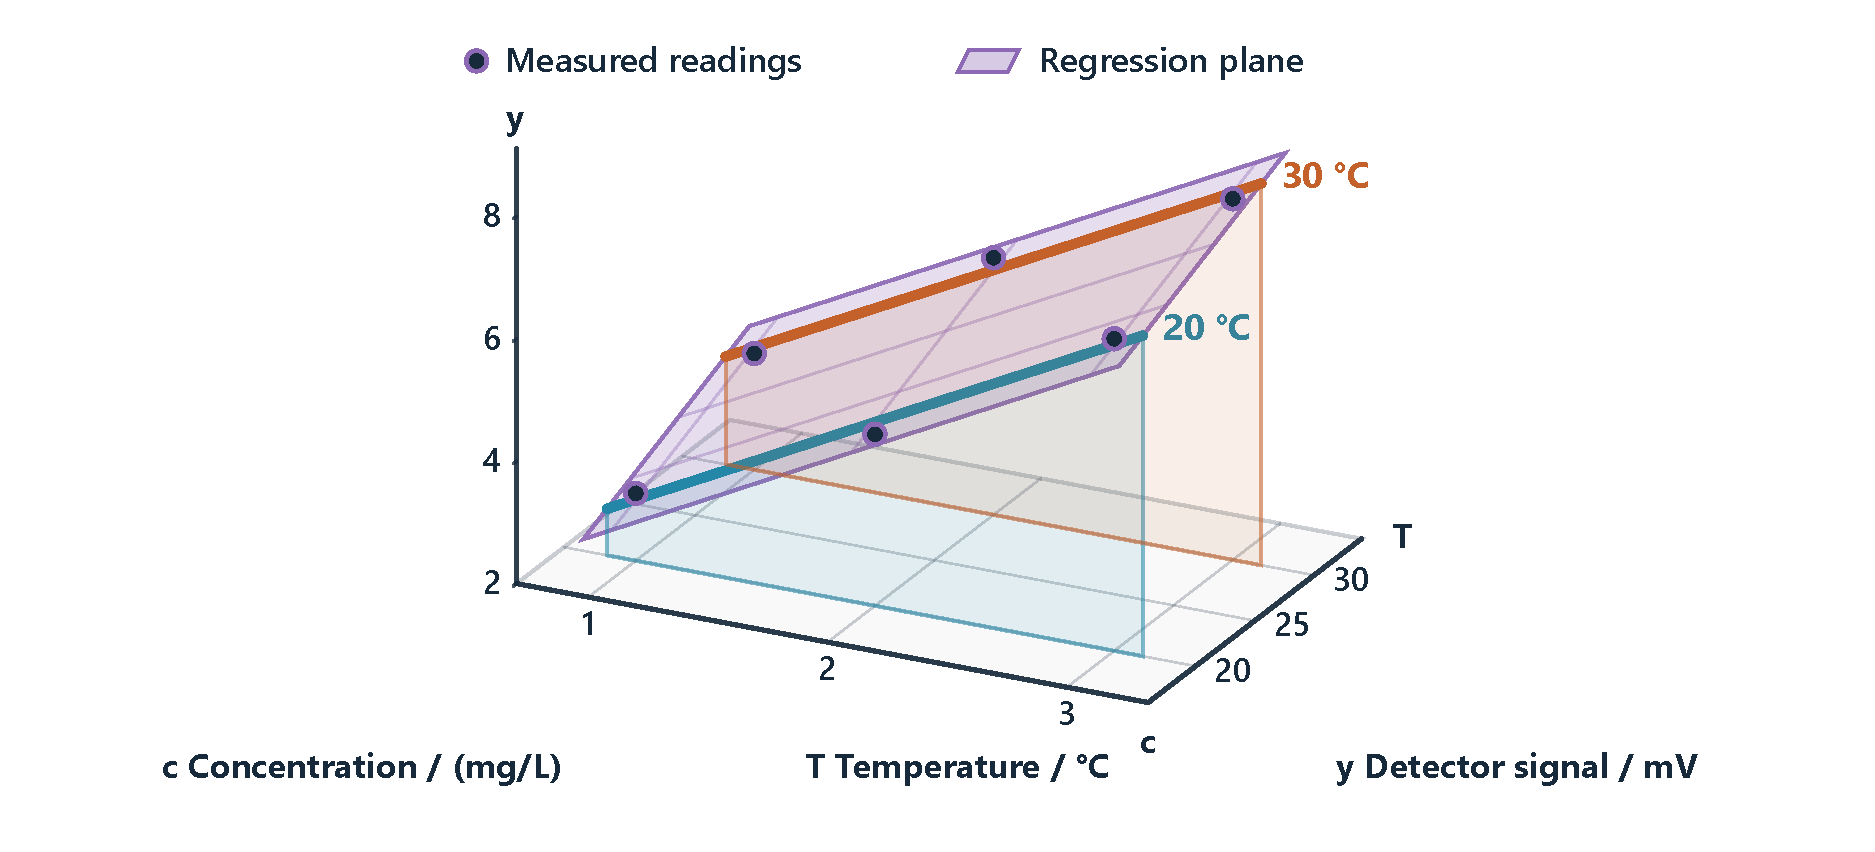
\includegraphics[width=\linewidth,height=.62\textheight,keepaspectratio]{asset-a622fdaf624cd167fb9129e176695b20f0efb5be89b04a0da51940a375eddd13.pdf}\end{center}

\medskip

\hyperref[material-a83c5e0bd863da6cc65b3623fcc23d11c0203629555b6ebaced359f4ddd64ca9]{Fig.~\ref*{material-a83c5e0bd863da6cc65b3623fcc23d11c0203629555b6ebaced359f4ddd64ca9}} plots the fitted signal against concentration at two fixed temperatures. The coefficient of concentration measures the change in fitted signal per mg/L while temperature stays fixed. The temperature coefficient measures the change per degree while concentration stays fixed. In \hyperref[material-253d534fc164cbd7b8f151c2039bb3fc58598d70b5d6e48e6a3ce52498a72284]{Eq.~\ref*{material-253d534fc164cbd7b8f151c2039bb3fc58598d70b5d6e48e6a3ce52498a72284}}, this works out to 2 mV per mg/L and 1 mV per 10 °C. The fitted profiles are parallel because the model assigns a common concentration slope to both temperatures. The next example uses the same regression with 0/1 predictors for a categorical variable.


\par\medskip
\Needspace{10cm}
\refstepcounter{figure}\label{material-a83c5e0bd863da6cc65b3623fcc23d11c0203629555b6ebaced359f4ddd64ca9}
\noindent\textbf{Fig.~\ref*{material-a83c5e0bd863da6cc65b3623fcc23d11c0203629555b6ebaced359f4ddd64ca9}.} What changes when we hold one predictor fixed?\par\nopagebreak
\begin{center}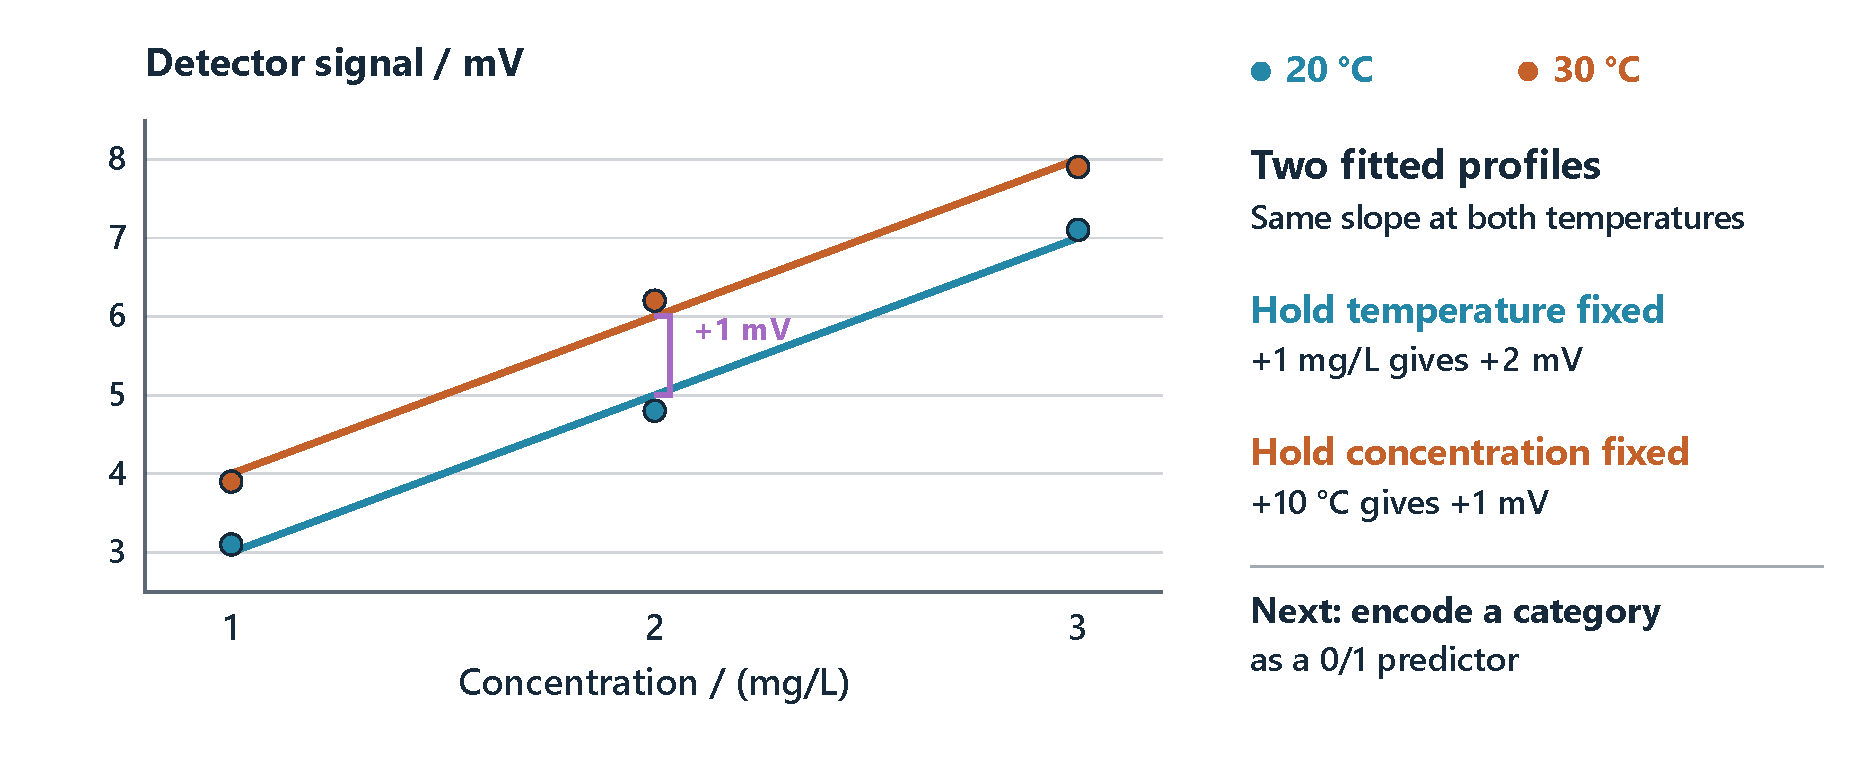
\includegraphics[width=\linewidth,height=.62\textheight,keepaspectratio]{asset-44ae25bb54d3fa34b44db343a4a28cadae83a0199fa6be52dac7aaebdb90fd40.pdf}\end{center}

\medskip

\par\medskip
\noindent\begin{minipage}{\linewidth}
\refstepcounter{equation}\label{material-253d534fc164cbd7b8f151c2039bb3fc58598d70b5d6e48e6a3ce52498a72284}
\noindent\textbf{Eq.~\ref*{material-253d534fc164cbd7b8f151c2039bb3fc58598d70b5d6e48e6a3ce52498a72284}.} Predict detector signal from two settings\par\nopagebreak
\begin{center}\begin{adjustbox}{max width=\linewidth}$\displaystyle \begin{aligned}\widehat y&=\beta_0+\beta_c c+\beta_T T\\&=-1.00+2.00c+0.10T\end{aligned}$\end{adjustbox}\end{center}

\par\noindent\textbf{Symbols}

\par\noindent\textbf{\(+,-,=\)} Addition, subtraction and equality. Adjacent factors multiply. The hat denotes a fitted value.

\par\noindent\textbf{\(-1.00,2.00,0.10\)} Fitted intercept, concentration slope and temperature slope, in that order.

\par\noindent\textbf{\(\widehat y,\beta_0,\beta_c,\beta_T\)} Fitted signal in mV. The intercept is in mV; the two slopes are in mV per mg/L and mV per °C.

\par\noindent\textbf{\(c,T\)} Measured concentration in mg/L and measured temperature in °C.

\end{minipage}\par
\medskip

\clearpage
\section{One-way ANOVA as a regression}
\textbf{One-way ANOVA as a linear regression}


The river-water SPE example from Level 7 has eighteen independent preparations, six per method. In \hyperref[material-60fe6339cdaad6295cc2ef25630ed0f89c036e6232067e10fd3f70628a0f3fdc]{Fig.~\ref*{material-60fe6339cdaad6295cc2ef25630ed0f89c036e6232067e10fd3f70628a0f3fdc}}, the response column contains the original recoveries. The design matrix has a column of ones and two 0/1 indicators, for methods B and C. Method A is the reference because both indicators are zero for its rows. An additional indicator for A would make the columns dependent, since the three indicators sum to the intercept column.


\par\medskip
\Needspace{10cm}
\refstepcounter{figure}\label{material-60fe6339cdaad6295cc2ef25630ed0f89c036e6232067e10fd3f70628a0f3fdc}
\noindent\textbf{Fig.~\ref*{material-60fe6339cdaad6295cc2ef25630ed0f89c036e6232067e10fd3f70628a0f3fdc}.} Turn three SPE methods into a design matrix\par\nopagebreak
\begin{center}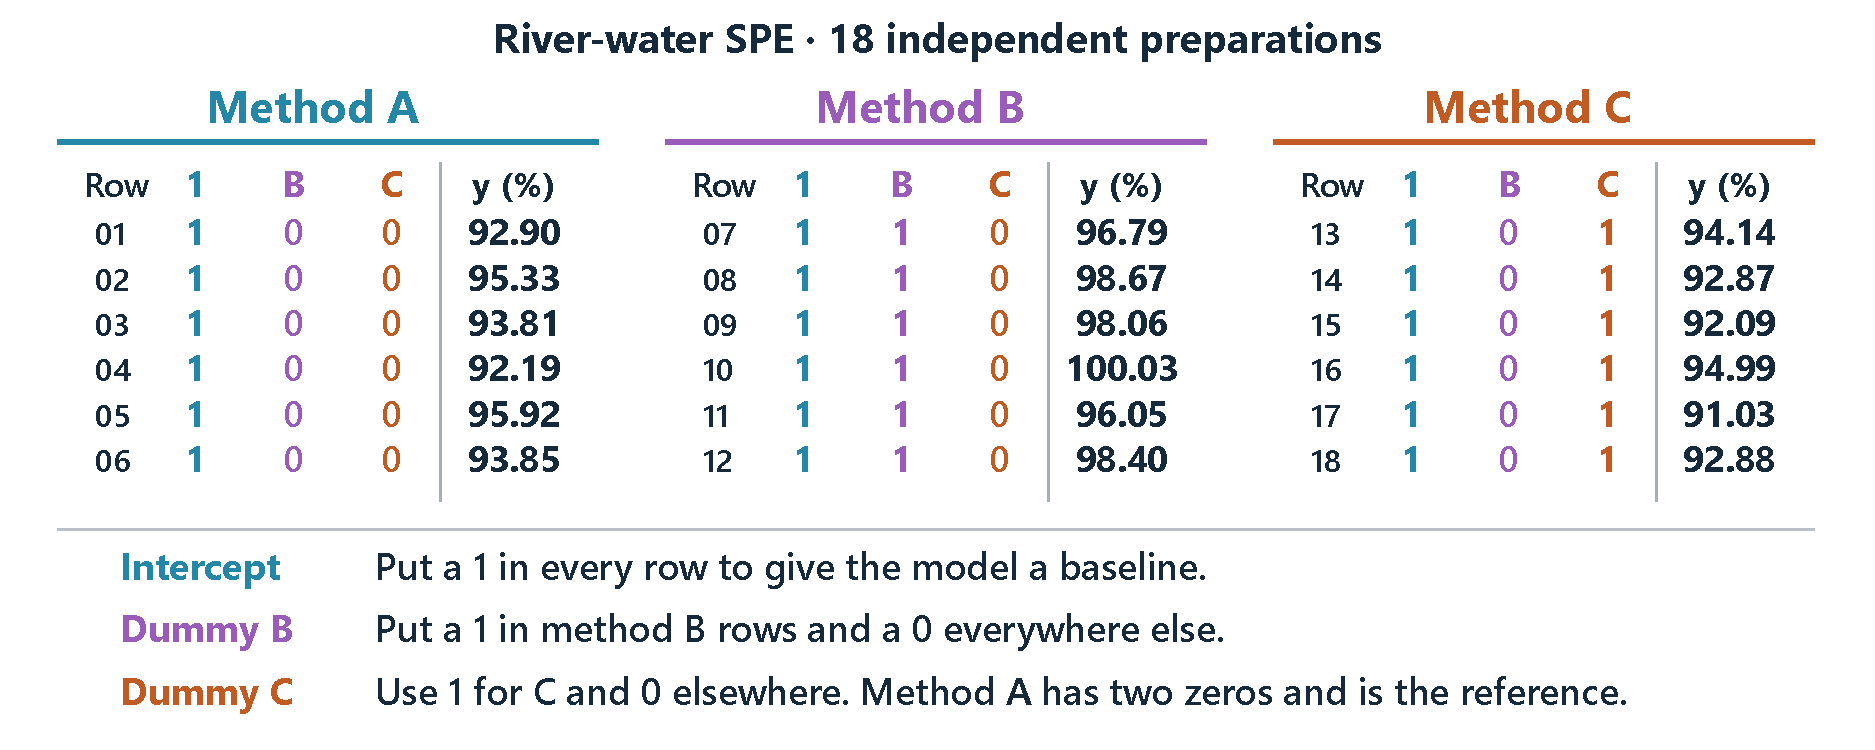
\includegraphics[width=\linewidth,height=.62\textheight,keepaspectratio]{asset-b99d9f256355f39516e227eddbef87699846017a06c2714d792604326a1cfbab.pdf}\end{center}

\medskip

In \hyperref[material-2634e6c47fcc38aa626bc6038a4de47156dd70586f6d601f23de9628250fba36]{Fig.~\ref*{material-2634e6c47fcc38aa626bc6038a4de47156dd70586f6d601f23de9628250fba36}}, the design rows are grouped by method and each pattern occurs six times. The products in \hyperref[material-06351facee15fd9cc149239ac963a4a6191f35d5f251a420030fe973b811f737]{Eq.~\ref*{material-06351facee15fd9cc149239ac963a4a6191f35d5f251a420030fe973b811f737}} show why the intercept counts 18, B and C each count six, and their overlap is zero. Multiplying by the observed responses sums 1710 across all preparations and selects the method totals 588 for B and 558 for C.


\par\medskip
\Needspace{10cm}
\refstepcounter{figure}\label{material-2634e6c47fcc38aa626bc6038a4de47156dd70586f6d601f23de9628250fba36}
\noindent\textbf{Fig.~\ref*{material-2634e6c47fcc38aa626bc6038a4de47156dd70586f6d601f23de9628250fba36}.} What do the dummy columns count and sum?\par\nopagebreak
\begin{center}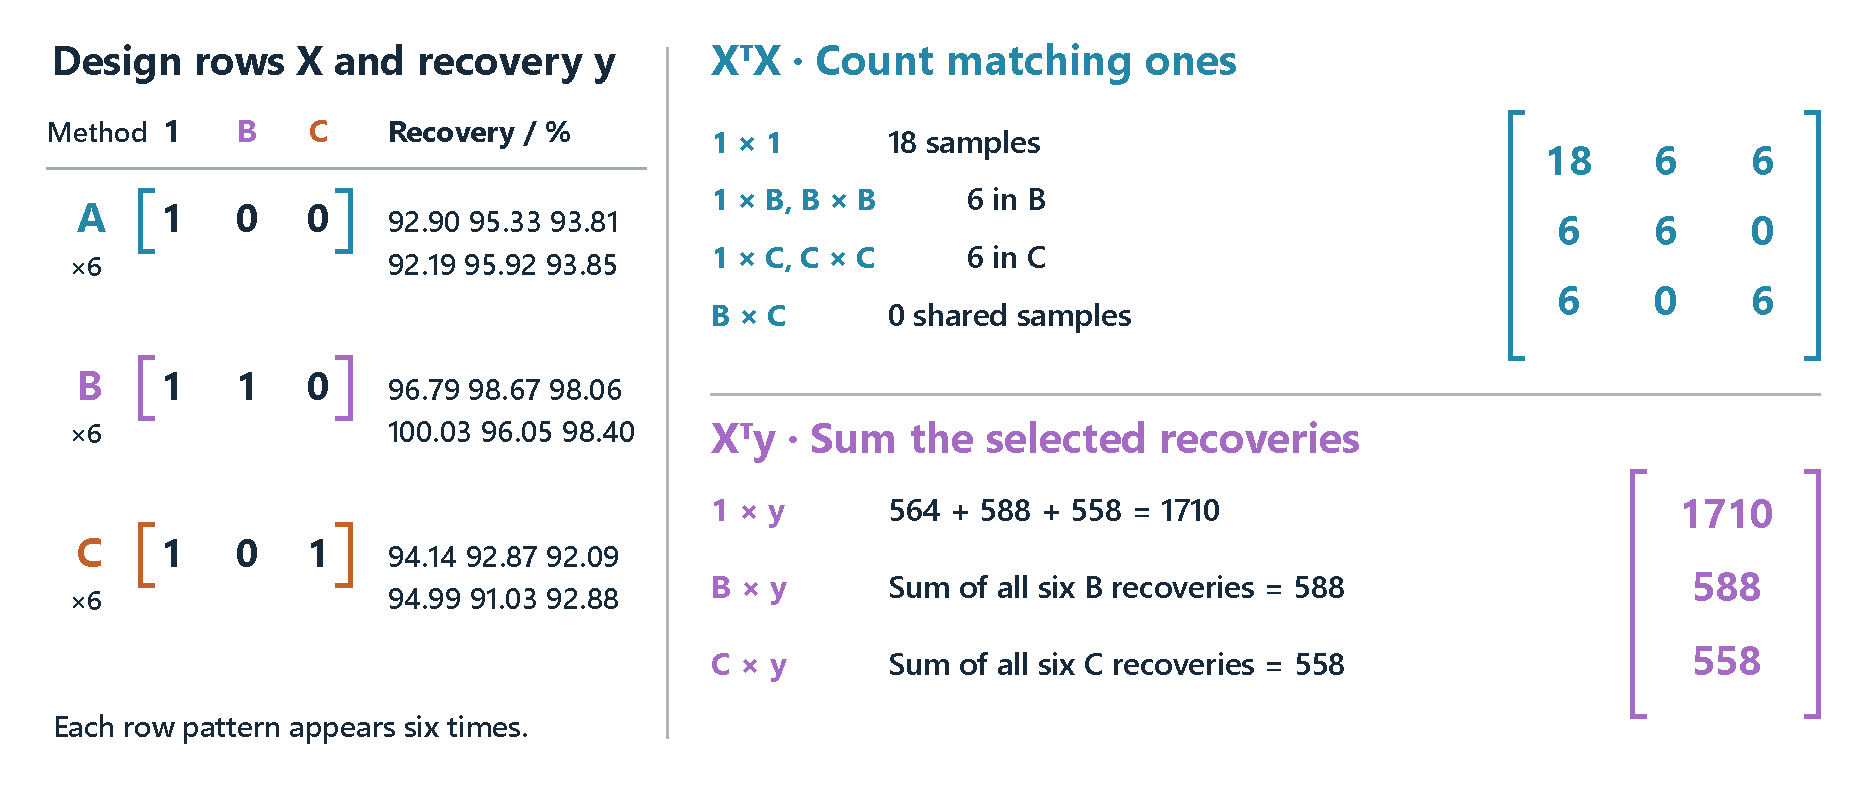
\includegraphics[width=\linewidth,height=.62\textheight,keepaspectratio]{asset-d5e84c6745bf5ca0b8ce1c7bb7db685a5fc6026364dd9979917379f09a26b227.pdf}\end{center}

\medskip

\par\medskip
\noindent\begin{minipage}{\linewidth}
\refstepcounter{equation}\label{material-06351facee15fd9cc149239ac963a4a6191f35d5f251a420030fe973b811f737}
\noindent\textbf{Eq.~\ref*{material-06351facee15fd9cc149239ac963a4a6191f35d5f251a420030fe973b811f737}.} Pair and sum the dummy columns\par\nopagebreak
\begin{center}\begin{adjustbox}{max width=\linewidth}$\displaystyle \begin{aligned}(X^{\mathsf T}X)_{jk}&=\sum_{i=1}^{18}X_{ij}X_{ik}\\[.45em](X^{\mathsf T}y)_j&=\sum_{i=1}^{18}X_{ij}y_i\end{aligned}$\end{adjustbox}\end{center}

\par\noindent\textbf{Symbols}

\par\noindent\textbf{\(X,y\)} Design matrix with columns for the intercept, method B, and method C. The vector contains the 18 original recovery measurements in \%.

\par\noindent\textbf{\(X_{ij},X_{ik},y_i\)} Two design entries in row i (0 or 1), and the measured recovery for that row.

\par\noindent\textbf{\(i,j,k\)} Row i refers to one preparation. Columns j and k select the intercept or one of the two method indicators.

\par\noindent\textbf{\({}^{\mathsf T},\sum,=\)} Transpose swaps rows and columns. Sum over all 18 preparations. Adjacent factors multiply and equals gives the resulting entry. Subscripts on parenthesised products identify the entry.

\end{minipage}\par
\medskip

\hyperref[material-d5eb31c6973de5593dc43c65aab7724a39fb8f3ce98e5f7bbea7748ab02928e4]{Eq.~\ref*{material-d5eb31c6973de5593dc43c65aab7724a39fb8f3ce98e5f7bbea7748ab02928e4}} applies the inverse to those sums. Its first row takes the total minus the B and C sums, leaving 564 for method A. Dividing by six gives 94\% recovery. The other two rows give the differences from A, +4 and \ensuremath{-}1 percentage points.


\par\medskip
\noindent\begin{minipage}{\linewidth}
\refstepcounter{equation}\label{material-d5eb31c6973de5593dc43c65aab7724a39fb8f3ce98e5f7bbea7748ab02928e4}
\noindent\textbf{Eq.~\ref*{material-d5eb31c6973de5593dc43c65aab7724a39fb8f3ce98e5f7bbea7748ab02928e4}.} Fit the recovery coefficients from the two products\par\nopagebreak
\begin{center}\begin{adjustbox}{max width=\linewidth}$\displaystyle \begin{aligned}\widehat\beta&=(X^{\mathsf T}X)^{-1}X^{\mathsf T}y=\textcolor{teal}{\begin{bmatrix}18&6&6\\6&6&0\\6&0&6\end{bmatrix}}^{-1}\textcolor{purple}{\begin{bmatrix}1710\\588\\558\end{bmatrix}}\\[.65em]&=\frac{1}{6}\begin{bmatrix}1&-1&-1\\-1&2&1\\-1&1&2\end{bmatrix}\begin{bmatrix}1710\\588\\558\end{bmatrix}=\begin{bmatrix}94\\4\\-1\end{bmatrix}\end{aligned}$\end{adjustbox}\end{center}

\par\noindent\textbf{Symbols}

\par\noindent\textbf{\(X,y\)} Design matrix with columns for the intercept, B and C, and the 18 recoveries in \%.

\par\noindent\textbf{\(\widehat\beta\)} Fitted coefficients in column order. First is the reference recovery for A (\%). The second and third are differences from A (percentage points).

\par\noindent\textbf{\({}^{\mathsf T},{}^{-1},=\)} Transpose swaps rows and columns. The exponent \ensuremath{-}1 inverts the whole matrix. Adjacent matrices and vectors multiply. Equals gives the evaluated result.

\end{minipage}\par
\medskip

\hyperref[material-cec37921a1aae4e1177ebd15405000f2f176f85e38b3bb97ccea5ebd58769255]{Fig.~\ref*{material-cec37921a1aae4e1177ebd15405000f2f176f85e38b3bb97ccea5ebd58769255}} compares two ordinary least-squares models. The intercept-only model predicts the grand mean (95\%) for every sample. The model with method predicts the mean of each group (94\%, 98\%, 93\%). With A as the reference, the fitted intercept is 94\% and the two adjustments are +4 and \ensuremath{-}1 percentage points. The null hypothesis of equal group means is the joint hypothesis that both adjustments are zero.


\par\medskip
\Needspace{10cm}
\refstepcounter{figure}\label{material-cec37921a1aae4e1177ebd15405000f2f176f85e38b3bb97ccea5ebd58769255}
\noindent\textbf{Fig.~\ref*{material-cec37921a1aae4e1177ebd15405000f2f176f85e38b3bb97ccea5ebd58769255}.} One-way ANOVA is a comparison of two regressions\par\nopagebreak
\begin{center}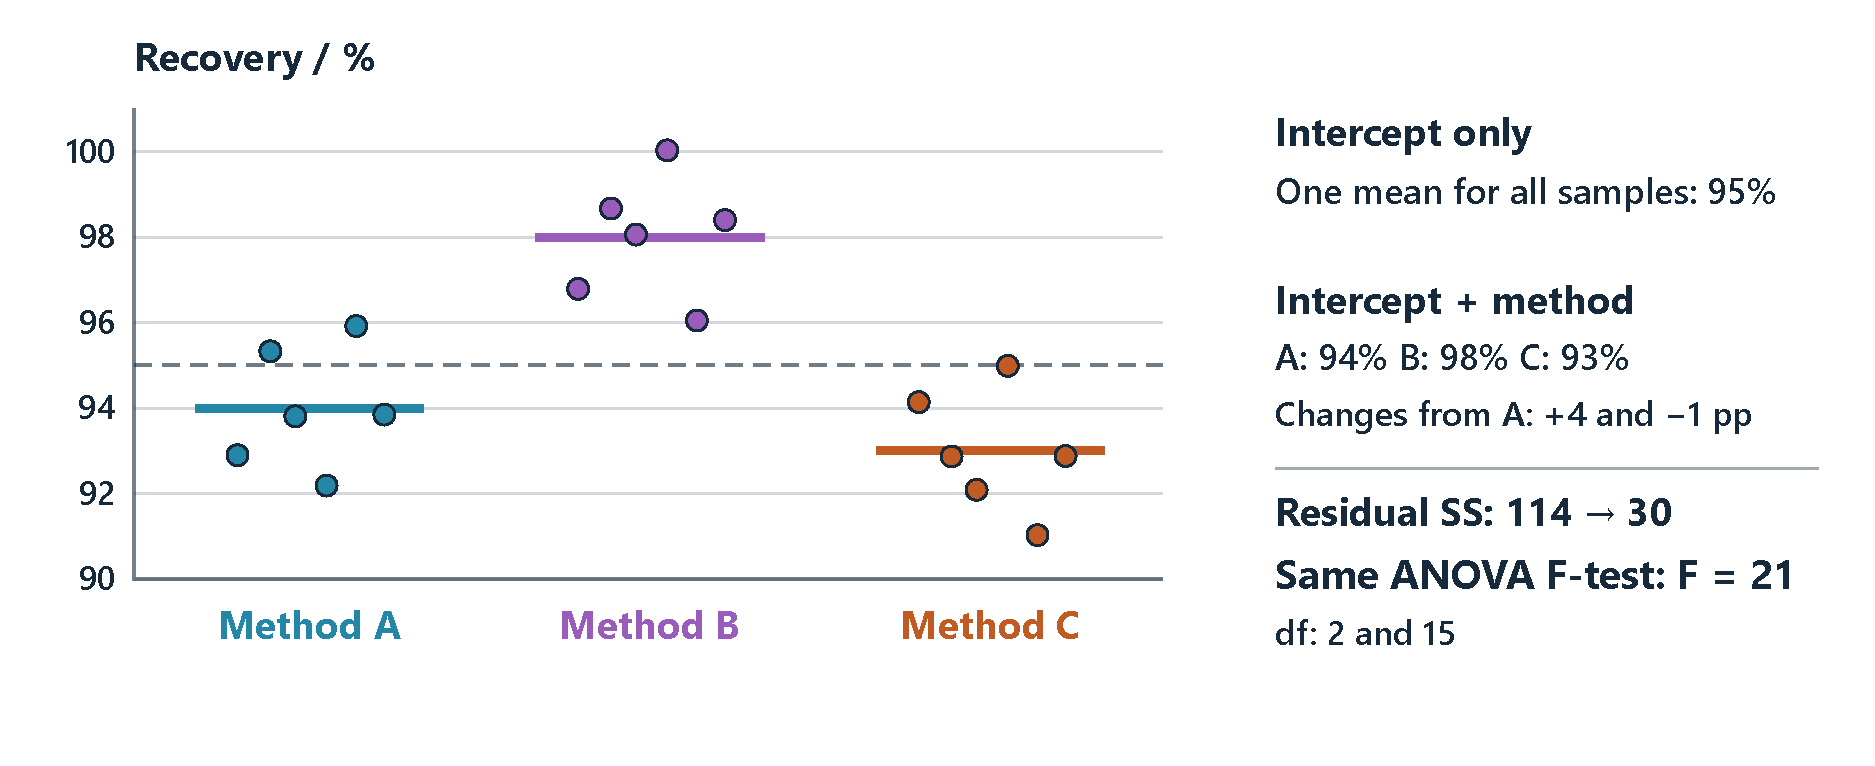
\includegraphics[width=\linewidth,height=.62\textheight,keepaspectratio]{asset-ef25715287c4993133b486bd616230be3bb9d5d0c8a972288b2482486d037940.pdf}\end{center}

\medskip

In \hyperref[material-a27755c7c29b0c4de2b1567c9199ef7f1dc1d94b864e777b8134ca7641675e63]{Eq.~\ref*{material-a27755c7c29b0c4de2b1567c9199ef7f1dc1d94b864e777b8134ca7641675e63}}, the drop in residual sum of squares from 114 to 30 is the between-method sum of squares, 84. The group model adds two coefficients and leaves fifteen residual degrees of freedom. Substitution in \hyperref[material-a27755c7c29b0c4de2b1567c9199ef7f1dc1d94b864e777b8134ca7641675e63]{Eq.~\ref*{material-a27755c7c29b0c4de2b1567c9199ef7f1dc1d94b864e777b8134ca7641675e63}} gives \(F=(84/2)/(30/15)=21\), the same statistic as one-way ANOVA. This comparison uses the classical ANOVA assumptions when interpreting the F test.


\par\medskip
\noindent\begin{minipage}{\linewidth}
\refstepcounter{equation}\label{material-a27755c7c29b0c4de2b1567c9199ef7f1dc1d94b864e777b8134ca7641675e63}
\noindent\textbf{Eq.~\ref*{material-a27755c7c29b0c4de2b1567c9199ef7f1dc1d94b864e777b8134ca7641675e63}.} Regression coefficients and the ANOVA F ratio\par\nopagebreak
\begin{center}\begin{adjustbox}{max width=\linewidth}$\displaystyle \begin{aligned}\widehat y&=\beta_0+\beta_B D_B+\beta_C D_C\\[.65em]F&=\frac{(SS_0-SS_1)/(\nu_0-\nu_1)}{SS_1/\nu_1}\end{aligned}$\end{adjustbox}\end{center}

\par\noindent\textbf{Symbols}

\par\noindent\textbf{\(+,-,=\)} Add, subtract and equal. Fraction bars divide. Parentheses group terms and adjacent factors multiply.

\par\noindent\textbf{\(F,SS_0,SS_1,\nu_0,\nu_1\)} F compares the intercept-only and method models. SS\ensuremath{{}_0} and SS\ensuremath{{}_1} are their residual sums of squares. The two \ensuremath{\nu} values are their residual degrees of freedom.

\par\noindent\textbf{\(\beta_0,\beta_B,\beta_C\)} Reference mean for method A (\%) and the two differences from that mean for B and C (percentage points).

\par\noindent\textbf{\(\widehat y,D_B,D_C\)} Fitted recovery in \%. The two indicators are 1 for their named method and 0 elsewhere. Both are zero for method A.

\end{minipage}\par
\medskip

\end{document}
